\chapter{柱、锥、台、球}

\section{柱、锥、台、球的定义及性质}
本节将研究由点、直线、平面等元素构成的几何体,常
见的几何体有柱、锥、台、球.

\subsection{柱}

柱面是经常遇到的物体的表面形状.建筑物的
棱柱、圆柱的侧面都是柱面,这些侧面可以看作是由一条直
线运动所产生的.

\begin{blk}{定义}
    一条直线$\ell$在空间作平行于固定方向的运动,但
总和任一固定的曲线$C$相交,所产生的曲面叫做柱面、移动
的直线$\ell$所在的每个位置叫做柱面的母线,而在移动中始终
和母线相交的曲线$C$叫做柱面的准线.
\end{blk}

下面,我们考虑几种简单情况
\begin{enumerate}
\item 准线是一条直线,这时的柱面是一个平面(见图
2.1).
\item 准线是一个平面多边形,这时的柱面叫做棱柱面
(见图2.2).
\item 准线是一个圆,这时的柱面叫做圆柱面(图2.3).
\end{enumerate}

\begin{figure}[htp]\centering
    \begin{minipage}[t]{0.3\textwidth}
    \centering
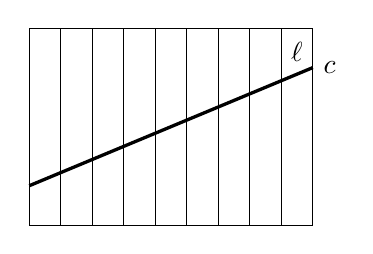
\begin{tikzpicture}[>=latex, scale=1]
\draw(0,0) rectangle (3.6,2.5);
\foreach \x in {.4,.8,1.2,...,2.8,3.2}
{
    \draw(\x,0)--(\x,2.5);
}
\draw[very thick](0,.5)--(3.6,2)node[right]{$c$};
\node at (3.2,2.2)[right]{$\ell$};
    \end{tikzpicture}
    \caption{}
    \end{minipage}
    \begin{minipage}[t]{0.3\textwidth}
    \centering
    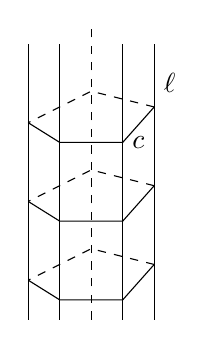
\begin{tikzpicture}[>=latex, scale=1]
\foreach \x in {0,.4,1.2,1.6}
{
    \draw(\x,0)--(\x, 3.5);
}
\draw[dashed](.8,0)--(.8, 3.7);
\foreach \x in {0,1,2}
{
    \draw(0,.5+\x)--(.4,.25+\x)--(1.2,.25+\x)--(1.6,.7+\x);
    \draw[dashed](1.6,.7+\x)--(.8,.9+\x)--(0,.5+\x);
}
\node at (1.6,3)[right]{$\ell$};
\node at (1.2,2.25)[right]{$c$};
    \end{tikzpicture}
    \caption{}
    \end{minipage}
        \begin{minipage}[t]{0.3\textwidth}
    \centering
    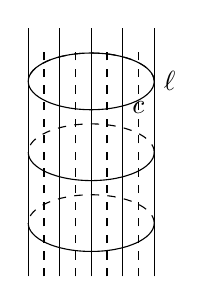
\begin{tikzpicture}[>=latex, yscale=.45]
\foreach \x in {0,.4,.8,1.2,1.6}
{
    \draw(\x,0)--(\x, 7);
}
\foreach \x in {.4,.8,1.2,1.6}
{
    \draw[dashed](\x-.2,0)--(\x-.2, 6.5);
}
\foreach \x in {1,2,3}
{
   \draw[dashed](1.6,-.5+\x*2) arc (0:180:.8);
   \draw (1.6,-.5+\x*2) arc (0:-180:.8);
}
\draw (1.6,-.5+3*2) arc (0:180:.8);
\node at (1.6,5.5)[right]{$\ell$};
\node at (1.6,5.2)[below left]{$c$};
    \end{tikzpicture}
    \caption{}
    \end{minipage}
    \end{figure}


以后我们只研究母线和该圆所在的平面垂直的圆柱面,
这种圆柱面叫\textbf{直圆柱面}.

\begin{blk}{定理}
    若平行平面与柱面的母线相交,则交线所成的图
形全等.
\end{blk}

\begin{proof}
    设平行平面$\alpha_1$和$\alpha_2$与柱面的母线相交,$\ell$是柱面上
任一条母线.令$P_1=\alpha_1\cap \ell$, $P_2=\alpha_2\cap\ell$, 我们称$P_1$和$P_2$是对
应点.显然$P_1$对应于$P_2$, $P_2$也对应于$P_1$, 并且不同位置的
两点$P_1$、$P'_1$对应于不同位置的两点$P_2$、$P_2'$(图2.4).

\begin{figure}[htp]
    \centering
	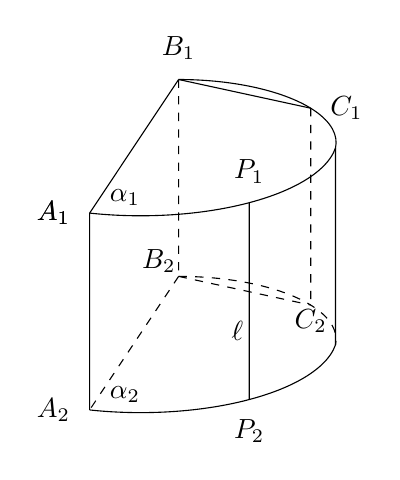
\begin{tikzpicture}[scale=1]
		\draw[dashed] (0,0) arc (90:-5:2 and 0.8) coordinate[pos=0.6](C2) coordinate[at end](X2);
		\draw (X2) arc (-8:-105:2.5 and 1) coordinate[pos=0.5](P2) coordinate[at end](A2);
		\draw[dashed] (0,0)--(A2);
		\draw (0,2.5) arc (90:-5:2 and 0.8) coordinate[pos=0.6](C1) coordinate[at end](X1);
		\draw (X1) arc (-8:-105:2.5 and 1) coordinate[pos=0.5](P1) coordinate[at end](A1);
		\draw (0,2.5)--(A1);
		\draw[dashed] (0,2.5)--(0,0) (C1)--(C2) (0,0)--(C2);
		\draw (0,2.5)--(C1) (A1)--(A2) (P1)--(P2) (X1)--(X2);
		\node[label=above:$B_1$] at (0,2.5) {};
		\node[label={[xshift=-0.25cm,yshift=-0.2cm]$B_2$}] at (0,0) {};
		\node[label=right:$C_1$] at (C1) {};
		\node[label={[yshift=-0.6cm]$C_2$}] at (C2) {};
		\node[label=above:$P_1$] at (P1) {};
		\node[label=below:$P_2$] at (P2) {};
		\node[label={[xshift=-0.15cm,yshift=0.5cm]$\ell$}] at (P2) {};
		\node[label=left:$A_1$] at (A1) {};
		\node[label=left:$A_2$] at (A2) {};
		\node[label=left:$A_1$] at (A1) {};
		\node[label={[xshift=0.45cm,yshift=-0.15cm]$\alpha_1	$}] at (A1) {};
		\node[label={[xshift=0.45cm,yshift=-0.15cm]$\alpha_2$}] at (A2) {};
	\end{tikzpicture}
    \caption{}
\end{figure}


于是在平行平面与柱面所截出的两条截线上的点与点之间建立了一一对应关系.

设在两条截线上有任意三对对应
点:$A_1$对应于$A_2$, $B_1$对应于$B_2$, $C_1$对
应于$C_2$, 因为$A_1A_2,B_1B_2,C_1C_2$都
是夹在平行平面$\alpha_1$和$\alpha_2$之间柱面的母
线的一部分,故
\[A_1A_2\mathop{=}^{\parallel} B_1B_2\mathop{=}^{\parallel}C_1C_2\]
从而四边形$A_1A_2B_2B_1$和四边形$B_1B_2C_2C_1$都是平行四边形,
它们的对边相等,所以,$A_1B_1=A_2B_2$, $B_1C_1=B_2C_2$. 又因
为$\angle A_1B_1C_1$与$\angle A_2B_2C_2$的两边平行且同向,所以
$\angle A_1B_1C_1=\angle A_2B_2C_2$.

这样,平行平面和柱面的母线相交,交出的图形总能重
合,因此它们全等.
\end{proof}


\begin{blk}{定义} 
    由封闭的柱面和两个与母线都相交的平行平面所
围成的几何体叫做柱体.

柱体的柱面夹在平行平面之间的部分叫做柱体的\textbf{侧面},
两个平行平面与柱体的相交部分叫做柱体的\textbf{底面}.
    
\end{blk}

现在,我们来研究几个特殊的柱体.

\begin{blk}{定义} 
    如果一个柱体的侧面是棱柱面,那么这个柱体叫
做棱柱.如果一个柱体的侧面是圆柱面,那么这个柱体叫圆
柱体.    
\end{blk}

显然,由这个定义可以得到以下推论:
\begin{enumerate}
\item 棱柱的两个底面是对应边互相平行的全等多边
形.

全等多边形的顶点叫做柱棱的顶点.以全等多边形对应
顶点为端点的线段称为棱柱的侧棱,相邻两侧棱及其所夹的
两底全等多边形的两条对应边所组成的四边形称为棱柱的侧
面.显然,
\item 棱柱的各侧面全是平行四边形.
\item 棱柱的各侧棱平行且相等.
\end{enumerate}


\begin{blk}{定义}
    棱柱按底面是三角形,四边形……分别叫做三棱
柱、四棱柱……

如果棱柱的侧棱垂直于底面,那么这个棱柱叫做直棱
柱,否则叫做斜棱柱.

如果棱柱是直棱柱,并且其底面是正多边形,那么这棱
柱就叫做正棱柱.在正棱柱中,各侧面都是全等的矩形.
\end{blk}
 
\begin{blk}
    {定义}棱柱上不在同一个底面上也不在同一个侧面上的
两个顶点所连结的线段叫做棱柱的对角线;过不在同一个
侧面的两条侧棱作一个平面,这平面截棱柱所得的截面叫做
棱柱的对角面.两底面之间的距离叫做棱柱的高.
\end{blk}

\begin{figure}[htp]
    \centering
\includegraphics[scale=.7]{fig/2-5.png}
    \caption{}
\end{figure}

图2.5是五棱柱,五边形$ABCDE$和$A'B'C'D'E'$是它
的两个底面,$ABB'A'$、$BCC'B'$等是它的侧面,$AA'$、$BB'$
等是它的侧棱,$HH'$的长是它的高.$A'C$是它的一条对角
线.

棱柱的表示法是写出两个底面各顶点
的字母,中间用一条短横线隔开,如图
2.5的五棱柱就表示作棱柱$ABCDE$-$A'
B'C'D'E'$. 也有用棱柱一条对角线的两
个端点表示棱柱的,如图2.5可表示作五
棱柱$A'C$. 

\begin{blk}{定义} 
    底面是平行四边形的四棱柱叫
    做平行六面体.其中侧棱和底面斜交的叫
    斜平行六面体,侧棱和底垂直的叫直平行六面体.底面是
    矩形的直平行六面体叫做长方体.交于一个顶点的三条棱的
    长相等的长方体叫做正方体,也叫立方体.(图2.6)
\end{blk}

\begin{figure}[htp]
    \centering
\begin{tikzpicture}
\begin{scope}
\tkzDefPoints{0/0/A, 1/0/B, 1.5/.5/C, .5/.5/D}
\tkzDefPoint(.25,2.2){A_1}
\tkzDefPointsBy[translation=from A to A_1](B,C,D){B_1,C_1,D_1}
\tkzDrawPolygon(A_1,B_1,C_1,D_1)
\draw(A)--(B)--(C);
\draw[dashed](A)--(D)--(C);
\draw[dashed](D_1)--(D);
\draw(A_1)--(A);\draw(B_1)--(B);\draw(C_1)--(C);
\node at (.5,-.5){斜平行六面体};
\end{scope}

\begin{scope}[xshift=3cm]
    \tkzDefPoints{0/0/A, .65/-.15/B, 2/0/C, 1.35/.15/D}
\tkzDefPoint(0,2){A_1}
\tkzDefPointsBy[translation=from A to A_1](B,C,D){B_1,C_1,D_1}
\tkzDrawPolygon(A_1,B_1,C_1,D_1)
\draw(A)--(B)--(C);
\draw[dashed](A)--(D)--(C);
\draw[dashed](D_1)--(D);
\draw(A_1)--(A);\draw(B_1)--(B);\draw(C_1)--(C);
\node at (0.75,-.5){直平行六面体};
\end{scope}

\begin{scope}[xshift=6cm]
    \tkzDefPoints{0/0/A, 1/0/B, 1.5/.5/C, .5/.5/D}
\tkzDefPoint(0,2.5){A_1}
\tkzDefPointsBy[translation=from A to A_1](B,C,D){B_1,C_1,D_1}
\tkzDrawPolygon(A_1,B_1,C_1,D_1)
\draw(A)--(B)--(C);
\draw[dashed](A)--(D)--(C);
\draw[dashed](D_1)--(D);
\draw(A_1)--(A);\draw(B_1)--(B);\draw(C_1)--(C);
\node at (.5,-.5){长方体};
\end{scope}

\begin{scope}[xshift=8.5cm]
    \tkzDefPoints{0/0/A, 1.5/0/B, 2/.5/C, .5/.5/D}
\tkzDefPoint(0,1.5){A_1}
\tkzDefPointsBy[translation=from A to A_1](B,C,D){B_1,C_1,D_1}
\tkzDrawPolygon(A_1,B_1,C_1,D_1)
\draw(A)--(B)--(C);
\draw[dashed](A)--(D)--(C);
\draw[dashed](D_1)--(D);
\draw(A_1)--(A);\draw(B_1)--(B);\draw(C_1)--(C);
\node at (1,-.5){正方体};
\end{scope}
\end{tikzpicture}
    \caption{}
\end{figure}




\begin{blk}
    {定义}
平行六面体中不含公共棱的两个面称为相对的
面.
\end{blk}

\begin{blk}{定理} 
   平行六面体相对的两个面全等,而它们所在的平
面互相平行. 
\end{blk}

已知:图2.7平行六面体$ABCD$-$A_1B_1C_1D_1$中,四边形
$ABB_1A_1$和$DCC_1D_1$是相对的两个面.

求证:$\parallelogram ABB_1A\cong \parallelogram DCC_1D_1$且平面$A_1B\parallel \text{平面}D_1C$.


\begin{figure}[htp]\centering
    \begin{minipage}[t]{0.48\textwidth}
    \centering
\begin{tikzpicture}[>=latex, scale=1.5]
    \tkzDefPoints{0/0/A, 2/0/B, 2.5/.5/C, .5/.5/D}
    \tkzDefPoint(.2,1){A_1}
    \tkzDefPointsBy[translation=from A to A_1](B,C,D){B_1,C_1,D_1}
    \tkzDrawPolygon(A_1,B_1,C_1,D_1)
    \draw(A)--(B)--(C);
    \draw[dashed](A)--(D)--(C);
    \draw[dashed](D_1)--(D);
    \draw(A_1)--(A);\draw(B_1)--(B);\draw(C_1)--(C);
    \tkzLabelPoints[left](A,D,A_1,D_1)
    \tkzLabelPoints[right](B,C,B_1,C_1)
    \end{tikzpicture}
    \caption{}
    \end{minipage}
    \begin{minipage}[t]{0.48\textwidth}
    \centering
    \begin{tikzpicture}[>=latex, scale=1.5]
        \tkzDefPoints{0/0/A, 2/0/B, 2.5/.5/C, .5/.5/D}
        \tkzDefPoint(0,1.5){A'}
        \tkzDefPointsBy[translation=from A to A'](B,C,D){B',C',D'}
        \tkzDrawPolygon(A,B,B',A')
        \draw(A')--(D')--(C')--(B');
        \draw(C')--(C)--(B);
        \draw[dashed](D')--(D)--(A);
        \draw[dashed](C)--(D)--(B');
        \draw[dashed](D)--(B);
        \tkzLabelPoints[left](A,D,A',D')
        \tkzLabelPoints[right](B,C,B',C')
    \end{tikzpicture}
    \caption{}
    \end{minipage}
    \end{figure}



\begin{proof}
    平行六面体的底面是平行四边形.

    $\therefore\quad AB\displaystyle\mathop{=}^{\parallel} DC$

    又$\because\quad$它的侧棱平行且相等,

    $\therefore\quad AA_1\displaystyle\mathop{=}^{\parallel} D_1D$

    $\therefore\quad \text{平面}A_1B {\parallel} \text{平面}D_1 C,\qquad \angle A_1AB=\angle D_1DC$

$\therefore\quad \parallelogram ABB_1A\cong \parallelogram DCC_1D_1$

同理,平面$A_1D\parallel\text{平面}B_1C,\qquad \parallelogram A_1 ADD_1\cong \parallelogram B_1BCC_1$.
\end{proof}

\begin{blk}
    {推论} 平行六面体的任何一对相对的面都可以作它的底
面.
\end{blk}

\begin{example}
    长方体的一条对角线的平方,等于通过同一顶点
的三条棱的平方和.

已知:长方体$DB'$中$DB'$是一条
对角线.(图2.8)

求证:${DB'}^2=AB^2+AD^2+{AA'}^2$
\end{example}

\begin{proof}
    连结$DB$

$\because\quad  AD\bot AB$

$\therefore\quad DB^2=AB^2+AD^2$

$\because B'B\bot\text{平面}AC,\quad DB\subset \text{平面}AC$
    
$\therefore\quad B'B\bot DB$

$\therefore\quad B'D^2={BB'}^2+BD^2$

$\because\quad AA'=BB'$

$\therefore\quad DB^2={AA'}^2+{BD}^2={AA'}^2+AB^2+AD^2$
\end{proof}

\begin{blk}
   {定理} 正棱柱两底中心的连线垂直于底面(请读者自证)
   
   圆柱体的两个底面是相等的圆面,它们所在的平
面平行.
\end{blk}

\begin{blk}{定义} 
    圆柱体两底面之间的距离叫做圆柱的高.

    圆柱体的母线平行且相等,并且垂直于两个底
面,母线的长等于圆柱的高.
\end{blk}

\begin{blk}{定义}
空间图形$F$对给定直线$\ell$为轴的轴对称是具有如
下性质的映射$R_1:F\mapsto F$, 对于任意点$P\in F$, 有它的像$R_1(P)
=P_1\in F$, 并且线段$PP'$被$\ell$垂直平分.这时$\ell$称为$F$的对
称轴.$P$、$P'$叫做关于$\ell$的对称点.

圆柱两底圆心连线垂直于底面,并且是圆柱的对
称轴(简称圆柱的轴).
\end{blk}

已知:如图2.9圆柱$AD$\footnote{圆柱可用它的两个底面内不在同一条母线上的两个点的字母来
表示.}中,
$O$、$O'$分别是两底上的圆心.

求证:
\begin{enumerate}
    \item $OO'$是圆柱$AD$的对称轴.
    \item $OO'$垂直两底.
\end{enumerate}

\begin{figure}[htp]
    \centering
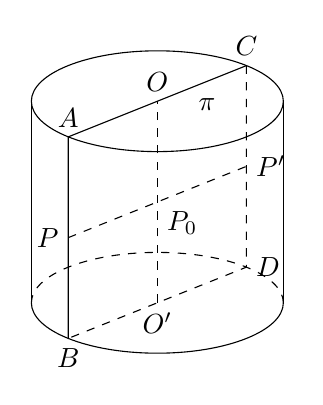
\begin{tikzpicture}[xscale=.8, yscale=.32]
\draw[dashed] (2,0) arc (0:180:2);
\draw (2,0) arc (0:-180:2);
\draw (0,8) circle (2);
\draw[dashed](1.414,1.414+8)--(1.414,1.414)node[right]{$D$}--(-1.414,-1.414);
\draw(1.414,1.414+8)node[above]{$C$}--(-1.414,-1.414+8)node[above]{$A$}--(-1.414,-1.414)node[below]{$B$};
\draw(-2,0)--(-2,8);\draw(2,0)--(2,8);
\node at (.5,.5+8)[below right]{$\pi$};
\draw[dashed](0,0)node [below]{$O'$}--(0,8)node [above]{$O$};
\draw[dashed](-1.414,-1.414+4)node[left]{$P$}--(1.414,1.414+4)node[right]{$P'$};
\node at (0,4)[below right]{$P_0$};
\end{tikzpicture}
    \caption{}
\end{figure}


\begin{proof}
\begin{enumerate}
    \item 

设点$P$是圆柱$AD$的柱面上
的任一点,过$P$作$PP_0\bot OO'$于$P_0$, 并且
$PP_0$的延长线交圆柱面于另一点$P'$.因为$PP'\cap OO'=P_0$, 所
以$PP'$、$OO'$确定一个平面$\pi$, $\pi$与圆柱面的交线为$AB$ ($P\in
AB$) 和$CD$ ($P'\in CD$), 与两底面的交线为$AC$ ($O\in AC$) 及
$BD$ ($O'\in BD$).

$\because\quad $圆柱的两个底面平行.

$\therefore\quad AC\parallel BD$ 且AC、BD分别为两底面圆的直径.

$\because\quad $圆柱的两底面是全等的圆面.

$\therefore\quad AC=BD\qquad ABDC$是平行四边形.

又$\because\quad AB$垂直两底面.

$\therefore\quad ABDC$为矩形,$\angle CAB=\angle ACD=90^{\circ}$

$\therefore\quad AO\displaystyle\mathop{=}^{\parallel}BO', OC\displaystyle\mathop{=}^{\parallel}O'D$

$\therefore\quad ABO'O$和$O'ODC$是两个全等的矩形

$\because\quad PP_0\bot OO'$于$P$.

$\therefore\quad PP_0=AO=OC=P_0P'$

$\therefore\quad PP'$被$OO'$垂直平分.

如果点$P$取在圆柱的底面上,那么它的像$P'$也在该圆面
上,同样可以证明$PP'$被$OO'$垂直平分.

$\therefore\quad OO'$是圆柱$AD$的对称轴.

\item 由1的证明可知,$OO'\parallel AB$, 而$AB$垂直于圆柱的两
个底面,所以$OO'$垂直于两底面.
\end{enumerate}
\end{proof}

\begin{blk}{定义}
    通过圆柱的轴的截面称为圆柱的轴截面.
\end{blk}

\begin{blk}{推论}
\begin{enumerate}
    \item 圆柱的轴截面是矩形.
    \item 过圆柱对称轴的平面是圆柱的对称平面.
    \item 平行于圆柱的轴的截面是矩形.
\end{enumerate}
\end{blk}

\begin{example}
    一圆柱用平行于圆柱的轴的平面去截它,截面周
界是30cm, 面积为54${\rm cm}^2$, 在底面上截得的一段弧为$120^{\circ}$, 求底面半径和圆柱的高.
\end{example}

\begin{figure}[htp]
    \centering
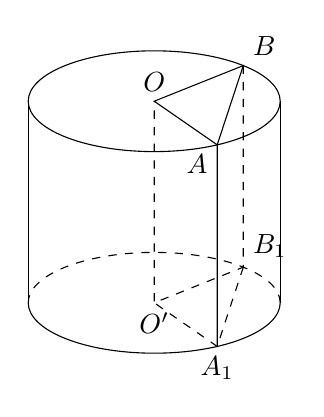
\begin{tikzpicture}[xscale=.8, yscale=.32]
\draw[dashed] (2,0) arc (0:180:2);
\draw (2,0) arc (0:-180:2);
\draw (0,8) circle (2);
\draw[dashed](1.414,1.414+8)node[above right]{$B$}--(1.414,1.414)node[above right]{$B_1$}--(0,0)node [below]{$O'$}--(0,8)node [above]{$O$};
\draw(-2,0)--(-2,8);\draw(2,0)--(2,8);
\draw[dashed](1.414,1.414)--(1,-1.732)node[below]{$A_1$}--(0,0);
\draw(1,-1.732)--(1,-1.732+8)--(0,8)--(1.414,1.414+8)--(1,-1.732+8)node[below left]{$A$};
\end{tikzpicture}
    \caption{}
\end{figure}

\begin{solution}
    如图2.10. 平行轴$OO'$的截面是矩形$AA_1B_1B$, 其边
$AB$是$\odot O$的弦,所对的圆心角是$120^{\circ}$, 故在$\triangle AOB$中,有
\[\frac{AB}{\sin 120^{\circ}}=\frac{R}{\sin 30^{\circ}}\]
其中$R$为$\odot O$的半径.

$\therefore\quad AB=\sqrt{3}R$

$\because\quad $矩形的另一边$AA_1$为圆柱的高,

$\therefore\quad AA_1=\frac{30}{2}-R\sqrt{3}$

又$\because\quad $矩形的面积为$54{\rm cm^2}$

$\therefore\quad R\sqrt{3}\left(15-R\sqrt{3}\right)=54 \quad \Rightarrow\quad R^2-5\sqrt{3}R+18=0$

解得:$R_1=3\sqrt{3},\quad R_2=2\sqrt{3}$,相应地圆柱高$h_1=6,\quad h_2=9$

答:圆柱底面半径为$3\sqrt{3}$cm, 高为
6cm, 或者半径为$2\sqrt{3}$cm, 高为9cm.
\end{solution}


\begin{ex}
\begin{enumerate}
    \item 柱面可视为准线沿母线方向连续平行移动时所占各位置
    的轨迹.用这句话说明棱柱、圆柱.
    \item 确定一个柱面需要几个条件?
    \item 从四棱柱、五棱柱和$n$棱柱的某一个顶点出发,各能引几
    条对角线?四棱柱、五棱柱和$n$棱柱各有几条对角线?
    \item \begin{enumerate}
    \item 平行六面体是斜四棱柱,斜四棱柱是不是平行六面
体?
\item 长方体是直四棱柱,直四棱柱是不是长方体?
\item 正方体是正四棱柱,正四棱柱是不是正方体?
    \end{enumerate} 

\item 有一个侧面是矩形的棱柱是不是直棱柱?有两个相对侧
面是矩形的$2n$棱柱呢?有两个相邻侧面是矩形的棱柱
呢?
\item 求证:和棱柱各侧棱相交的两个平行截面是两个全等的
多边形.
\item 求证:用平行于圆柱的底面的平面去截圆柱所得的截面
是和底面相等的圆面.
\item 一个圆柱体有多少个对称轴?有多少个对称平面?
\item 用第一种画法画正六棱柱的直观图,用第二种画法画圆
柱的直观图.
\end{enumerate}  
\end{ex}

\subsection{锥}

在前面我们初步地讨论了柱(包括棱柱和圆
柱)的定义及其某些性质.这一节将研究锥(包括棱锥和圆
锥)的定义及其性质,我们从锥面说起.

\subsubsection{锥面}

\begin{blk}
    {定义} 给定平面曲线$C$和$C$所在平面外一点$S$, 设直线$\ell$
经过$S$点运动并且总和$C$相交,则运动的直线$\ell$所产生的曲面
叫做锥面.$S$点叫做锥面的顶点,运动着的直线$\ell$的每一位置
叫作锥面的母线,而在运动中始终和母线相交的曲线$C$叫做
锥面的准线.
\end{blk}

通常,我们只讨论通过顶点$S$总和准线$C$相交的射线运
动时所产生的锥面.

下面我们来考虑几种简单情况:
\begin{enumerate}
    \item 准线是一条线段,这时锥面是一个平面区域,其边
    界是一个角.(图2.11)
    \item 准线是一个多边形,这时的锥面叫\textbf{多面角}.它是由
    从顶点出发通过多边形的各个顶点作射线,这些射线以及每
    两条相邻射线间平面部分所组成的图形.(图2.12)

    通过多边形顶点的母线叫作多面角的\textbf{棱}.锥面的顶点叫
    做多面角的\textbf{顶点}.相邻两棱的平面部分叫做多面角的\textbf{面},在
    每个面内由两条棱组成的角叫作多面角的\textbf{面角}.
    \item 准线是个圆,如果圆面垂直于连接顶点和圆心的直
    线,那么锥面叫作直圆锥面,简称圆锥面.(图2.13)通过
    顶点和准线圆中心的直线是圆锥面的轴.锥面的表示法可以
    用它的顶点字母$S$表示,记作锥面$S$. 也可表示成锥面$S-
    ABCDE$等其中$A,B,C,D,E$等分别是锥面上不同母线上的
    点.
\end{enumerate}

\begin{figure}[htp]\centering
    \begin{minipage}[t]{0.3\textwidth}
    \centering
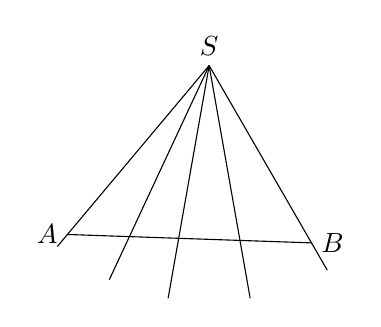
\begin{tikzpicture}[>=latex, scale=1]
    \foreach \x in {-60,-80,-100,-115,-130}
    {
        \draw(0,0)--(\x:3);
    }
    \node at (0,0)[above]{$S$};
    \draw(-130:2.8)node[left]{$A$}--(-60:2.6)node[right]{$B$};
    \end{tikzpicture}
    \caption{}
    \end{minipage}
    \begin{minipage}[t]{0.38\textwidth}
    \centering
    \begin{tikzpicture}[>=latex, scale=1]
\tkzDefPoints{0/0/A, 1.5/0/B, 2/.5/C, .8/1/D, -.5/.6/E, .8/2.5/S}
\draw(E)--(A)--(B)--(C);
\draw [dashed](C)--(D)--(E);
\tkzDrawLines[add=0 and .5](S,E S,A S,B S,C)
\tkzDrawLines[add=0 and 1, dashed](S,D)
\tkzLabelPoints[below](A,B)
\tkzLabelPoints[above](C,D,E,S)

    \end{tikzpicture}
    \caption{}
    \end{minipage}
    \begin{minipage}[t]{0.25\textwidth}
    \centering
    \begin{tikzpicture}[>=latex, yscale=.4]
        \draw[dashed] (1,0) arc (0:180:1);
        \draw (1,0) arc (0:-180:1);
\tkzDefPoints{1/0/A, -1/0/B, 0/6/S, 0/0/O}
\tkzDrawLines[add=0 and .5](S,A S,B)
\tkzDrawLines[add=0 and .35, dashed](S,O)
\draw(S)--+(-95:9);
\tkzLabelPoints[above](S,O)
    \end{tikzpicture}
    \caption{}
    \end{minipage}
    \end{figure}

\begin{blk}
    {定理} 不通过顶点$S$的两个平行平面与锥面相交,所
    得到的图形相似,其相似比等于顶点到两平行平面的距离之
    比.
\end{blk}

已知:锥面$S$-$ABC\cdots$, 平行平面$\alpha_1$与$\alpha_2$都不通过顶
点$S$与锥面相交,得到截面图形$F_1$(在$\alpha_1$上)与$F_2$(在$\alpha_2$上),
又$SO_1\bot\alpha_1$于$O_1$, $SO_2\bot\alpha_2$于$O_2$(图2.14).

求证:截面图形$F_1\backsim F_2$, 其相似比
$K=\frac{SO_1}{SO_2}$。

\begin{figure}[ht]
    \centering
	\tdplotsetmaincoords{75}{0}
	\begin{tikzpicture}[scale=0.8,tdplot_main_coords]
		\def\zone{1.5}
		\def\ztwo{2.5}
		\pgfmathsetmacro{\zratio}{\ztwo/\zone}
		\coordinate (S) at (0,0,{-\zone + \zone*1.5/(\ztwo/\zone-1)});
		\coordinate (O1) at (0,0,-\zone);
		\coordinate (O2) at (0,0,-\ztwo*1.5);
		\draw[dashed] (S)--($(S)!1.15!(O2)$);
		\draw ($(S)!1.15!(O2)$)--($(S)!1.4!(O2)$);
		\node[label=above:$S$] at (S) {};
		\begin{scope}[canvas is xy plane at z={-\zone}]
			\draw ({-1.5*\zratio},{2*\zratio})--({-2.5*\zratio},{-2*\zratio})--({1.5*\zratio},{-2*\zratio})--({2.5*\zratio},{2*\zratio})--cycle;
			\draw[dashed] plot[domain=-1:1,variable=\t] (\t, {1+0.3*sin(\t*270-90)});
			\draw[dashed] (-1,1) arc (-225:-180:1.4142) coordinate[at end](westend);
			\draw[dashed] (1,1) arc (45:0:1.4142) coordinate[at end](eastend);
			\draw (westend) arc (-180:0:1.4142) coordinate[pos=0.2](X1) coordinate[pos=0.6](Y1) coordinate[pos=0.7](Z1);
			\draw[dashed] (O1)--(X1)--(Y1)--cycle;
			\node[label={[xshift=-0.1cm,yshift=-0.6cm]$X_1$}] at (X1) {};
			\node[label={[xshift=-0.2cm,yshift=-0.2cm]$O_1$}] at (O1) {};
			\node[label={[xshift=0.2cm,yshift=-0.6cm]$Y_1$}] at (Y1) {};
			\node[label=right:$F_1$] at (eastend) {};
			\node[label={[xshift=-0.5cm,yshift=-0.55cm]$\alpha_1$}] at ({2.5*\zratio},{2*\zratio}) {};
		\end{scope}
		\begin{scope}[canvas is xy plane at z={-\ztwo*1.5}]
			\draw ({-2*\zratio},{2*\zratio})--({-3*\zratio},{-2*\zratio})--({2*\zratio},{-2*\zratio})--({3*\zratio},{2*\zratio})--cycle;
			\draw[dashed] plot[domain={-\zratio}:\zratio,variable=\t] (\t, {(1+0.3*sin(\t/\zratio*270-90))*\zratio});
			\draw[dashed] (-\zratio,1*\zratio) arc (-225:-180:{1.4142*\zratio}) coordinate[at end](westend2);
			\draw[dashed] (\zratio,1*\zratio) arc (45:0:{1.4142*\zratio}) coordinate[at end](eastend2);
			\draw (westend2) arc (-180:0:{1.4142*\zratio}) coordinate[pos=0.2](X2) coordinate[pos=0.6](Y2) coordinate[pos=0.7](Z2);
			\draw[dashed] (O2)--(X2)--(Y2)--cycle;
			\node[label={[xshift=-0.1cm,yshift=-0.6cm]$X_2$}] at (X2) {};
			\node[label={[xshift=-0.3cm,yshift=-0.6cm]$O_2$}] at (O2) {};
			\node[label={[xshift=0.2cm,yshift=-0.6cm]$Y_2$}] at (Y2) {};
			\node[label=right:$F_2$] at (eastend2) {};
			\node[label={[xshift=-0.5cm,yshift=-0.55cm]$\alpha_2$}] at ({3*\zratio},{2*\zratio}) {};
		\end{scope}
		\draw (S)--(westend);
		\draw[dashed] (westend)--($(S)!1.15!(westend)$);
		\draw ($(S)!1.15!(westend)$)--(westend2);
		\draw[dashed] (westend2)--($(S)!1.15!(westend2)$);
		\draw ($(S)!1.15!(westend2)$)--($(S)!1.5!(westend2)$) node[at end,below] (westendExt) {$A$};
		
		\draw (S)--(eastend);
		\draw[dashed] (eastend)--($(S)!1.15!(eastend)$);
		\draw ($(S)!1.15!(eastend)$)--(eastend2);
		\draw[dashed] (eastend2)--($(S)!1.15!(eastend2)$);
		\draw ($(S)!1.15!(eastend2)$)--($(S)!1.4!(eastend2)$) node[at end,below] (eastendExt) {$C$};
		
		\draw (S)--(X1);
		\draw[dashed] (X1)--($(S)!1.1!(X1)$);
		\draw ($(S)!1.1!(X1)$)--(X2);
		\draw[dashed] (X2)--($(S)!1.1!(X2)$);
		\draw ($(S)!1.1!(X2)$)--($(S)!1.4!(X2)$) node[at end,below] (XExt) {$X$};
		
		\draw (S)--(Y1); 	\draw[dashed] (Y1)--($(S)!1.06!(Y1)$);	\draw ($(S)!1.06!(Y1)$)--(Y2);	\draw[dashed] (Y2)--($(S)!1.06!(Y2)$);	\draw ($(S)!1.06!(Y2)$)--($(S)!1.35!(Y2)$) node[at end,below] (YExt) {$Y$};
		
		\draw (S)--(Z1); 	\draw[dashed] (Z1)--($(S)!1.15!(Z1)$);	\draw ($(S)!1.15!(Z1)$)--(Z2);	\draw[dashed] (Z2)--($(S)!1.08!(Z2)$);	\draw ($(S)!1.08!(Z2)$)--($(S)!1.35!(Z2)$)  node[at end,below] (ZExt) {$B$};;
	\end{tikzpicture}
    \caption{}
\end{figure}

\begin{proof}
任引锥面$S$-$ABC\cdots$的一条母线$SX$, 由于$F_1$
和$F_2$都是锥面的截面,所以$SX$
必与$F_1$和$F_2$分别交于$X_1$和$X_2$两
点,这时,$X_2$可以看成$F_1$上$X_1$的
对应点,$X_1$也可看成是$F_2$上$X_2$
的对应点.

如果另外再取一条不同于
$SX$的母线$SY$, 同样可以得到
$F_1$和$F_2$上的另一对对应点$Y_1$和
$Y_2$, 显然$X_1\ne Y_1$, $X_2\ne Y_2$, 否
则$SX$与$SY$重合,这将与它们
是不同的母线相矛盾.因此,
$F_1$和$F_2$的点与点之间建立了一一对应关系.

又设$SX$和$SY$所确定的平面为$\pi$, 则$\pi\cap \alpha_1=X_1Y_1$,
$\pi\cap \alpha_2=X_2Y_2$, 因为$\alpha_1\parallel \alpha_2$, 所以$X_1Y_1\parallel X_2Y_2$. 因此:
\begin{equation}
    \frac{X_1Y_1}{X_2Y_2}=\frac{SX_1}{SX_2}
\end{equation}
连结$X_1O_1$, $X_2O_2$, 并令$SX$与$SO_2$所确定的平面为$\pi'$, 
则$\pi'\cap\alpha_1=X_1O_1$, $\pi'\cap\alpha_2=X_2O_2$

$\because\quad \alpha_1\parallel \alpha_2$

$\therefore\quad X_1O_1\parallel X_2O_2$
\begin{equation}
    \frac{SX_1}{SX_2}=\frac{SO_1}{SO_2}
\end{equation}
由(2.1), (2.2)有:
\[\frac{X_1Y_1}{X_2Y_2}=\frac{SO_1}{SO_2}=K\quad\text{(常数)}\]
由相似图形的定义可知:
\[F_1\backsim F_2,\quad \text{并且相似比}K=\frac{SO_1}{SO_2}\]
\end{proof}

\subsubsection{棱锥与圆锥}
\begin{blk}
   {定义} 如果一个锥面的准线是一条封闭曲线则称这个锥
面为封闭锥面.如圆锥面、多面角都是封闭锥面.

如果一个封闭锥面的所有线被一个平面所截,那么由
这个截面和锥面所围成的几何体叫做锥体.锥体平面部分叫
作锥体的底面,顶点和底面的距离叫做锥体的高. 
\end{blk}

下面我们讨论几个特殊的锥体.

\begin{blk}
    {定义}如果一个多面角的所有的棱被一个平面所截,那
么截面和多面角各面所围成的几何体叫作棱锥.原多面角的
顶点叫做棱锥的顶点,截面和多面角相交的部分显然是多边
形,它所围的平面部分叫做棱锥的底面,有公共顶点的各个
三角形的面叫做棱锥的侧面,两个相邻侧面的公共边叫做棱
锥的棱侧.

如果棱锥的底面是三角形、四边形……$n$边形,那么棱锥
就分别叫做\textbf{三棱锥、四棱锥、五棱锥……$n$棱锥}(见图2.15)、棱锥的表示法可以用表示顶点和底面顶点的
几个字母来表示,例如棱锥$S-ACD$. 
\end{blk}

如果棱锥的底面是正多边形,并且由棱锥顶点到它的底
面的垂线经过这个多边形的中心,那么这个棱锥就叫作\textbf{正棱
锥}.

\begin{figure}[htp]
    \centering
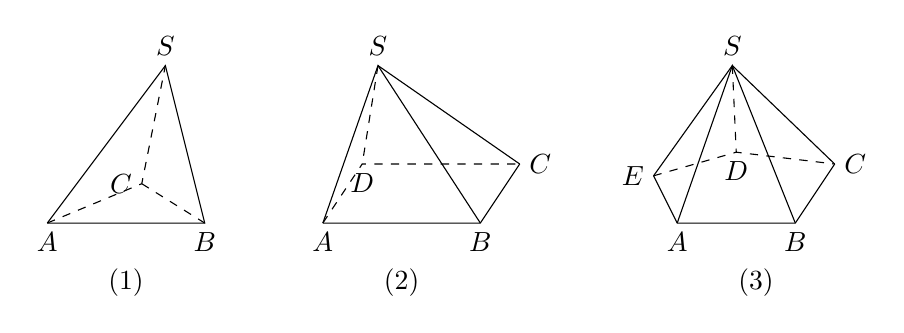
\begin{tikzpicture}
\begin{scope}
\draw(0,0)node[below]{$A$}--(2,0)node[below]{$B$}--(1.5,2)node[above]{$S$}--(0,0);
\draw[dashed](0,0)--(1.2,.5)node[left]{$C$}--(1.5,2);
\draw[dashed](1.2,0.5)--(2,0);
\node at (1,-.75){(1)};

\end{scope}
\begin{scope}[xshift=3.5cm]
    \draw(0,0)node[below]{$A$}--(2,0)node[below]{$B$}--(2.5,.75)node[right]{$C$};
\draw[dashed](0,0)--(.5,.75)node[below]{$D$}--(2.5,.75);
\draw(0,0)--(.7,2)node[above]{$S$}--(2,0);
\draw(.7,2)--(2.5,.75);
\draw[dashed](.7,2)--(.5,.75);
\node at (1,-.75){(2)};
\end{scope}
\begin{scope}[xshift=8cm]
    \draw(-.3,.6)node[left]{$E$}--(0,0)node[below]{$A$}--(1.5,0)node[below]{$B$}--(2,.75)node[right]{$C$};
    \draw(0,0)--(.7,2)node[above]{$S$}--(1.5,0);
    \draw(-.3,.6)--(.7,2)--(2,.75);

    \draw[dashed](-.3,.6)--(.75,.9)node[below]{$D$}--(2,.75);
\draw[dashed](.7,2)--(.75,.9);
    \node at (1,-.75){(3)};
\end{scope}
\end{tikzpicture}
    \caption{}
\end{figure}


图2.16是用第一种画法画出的正六棱锥的直观图.
\begin{figure}[htp]
    \centering
\includegraphics[scale=.55]{fig/2-16.png}
    \caption{}
\end{figure}

正棱锥显然有如下的性质:
\begin{enumerate}
\item 正棱锥所有的侧棱都相等.
\item 正棱锥过顶点的所有面角都相等.
\item 正棱锥各个侧面是全等的等腰三角形.

因为全等的等腰三角形底边上的高都相等,所以正棱锥侧面的等腰三角形底边上的高都叫作
正棱锥的\textbf{斜高}.例如图2.16(3)中$\triangle SBC$底边$BC$上的高$SG$就
是正棱锥$S-AD$的斜高.
\item 正棱锥所有的斜高都相等.
\item 正棱锥的棱、高、及棱在底上的射影以及斜高、高
和斜高在底面上的射影分别组成一个直角三角形.
\end{enumerate}

我们已经看到正棱锥的许多元素,如侧棱、底边(底面
正多边形的边)、高、斜高、侧棱和底面的夹角、侧面和底
面所成的角、斜高和高所成的角等等.在这些元素中只要给
出其中两个元素(至少有一线段),就可以通过解直角三角
形和底面正多边形来求出其它元素.

\begin{example}
已知棱锥底面是边长为12的三角形,它的各个侧
面和底面成$45^{\circ}$角,
\begin{enumerate}
    \item 求证这个棱锥是正三棱锥;
    \item 求这个三棱锥的高.
\end{enumerate}

已知:在棱锥$S$-$ABC$中,$AB=BC=CA=12$cm, 
面$SAB$、$SBC$、$SCA$都和底面$ABC$成$45^{\circ}$角.
\begin{enumerate}
    \item 求证:$S$-$ABC$是正三棱锥;
    \item 求三棱锥的高$SO$.
\end{enumerate}
\end{example}

\begin{solution}
    设$SO$为三棱锥的高,过$O$点在底面内作$OD$、$OE$、
$OF$分别垂直于$\triangle ABC$的各边$AB$、$BC$、$CA$, 连接$SD$、$SE$、
$SF$, 则$SD\bot BA$, $SE\bot BC$, $SF\bot AC$ (三垂线定理)(见图2.17), 即$\angle SDO$, $\angle SEO$, $\angle SFO$分别是棱锥各个侧
面和底面所成二面角的平面角.

$\therefore\quad \angle SDO=\angle SEO=\angle SFO=45^{\circ}$

从而$\triangle SOD\cong \triangle SOE\cong \triangle SOF$,
于是$OD=OE=OF$.

即:$O$点是$\triangle ABC$的内心,又因为正三角形的内心、外
心、重心、垂心重合,所以三棱锥$S$-$ABC$是正三棱锥.

又$OD=\frac{1}{3}CD=\frac{1}{3}\sqrt{CB^2-BD^2}=\frac{1}{3}\sqcup12^2-6^2=\frac{1}{3}\x 6\sqrt{3}=2\sqrt{3}$

$\because\quad \triangle SOD$是等腰直角三角形

$\therefore\quad SO=OD=2\sqrt{3}$ (cm)

答:棱锥的高为$2\sqrt{3}$cm.
\end{solution}

\begin{figure}[htp]\centering
    \begin{minipage}[t]{0.48\textwidth}
    \centering
\begin{tikzpicture}
\tkzDefPoints{0/0/A, 3/0/B, 4/1.5/C, 2/3/S, 2.3/.5/O}
\tkzDefMidPoint(A,B) \tkzGetPoint{D}
\tkzDefMidPoint(A,C) \tkzGetPoint{F}
\tkzDefMidPoint(C,B) \tkzGetPoint{E}
\tkzDrawSegments(A,B B,C S,A S,B S,C S,D S,E)
\tkzDrawSegments[dashed](A,C S,F F,B C,D A,E S,O)
\tkzLabelPoints[below](A,D,B,O)
\tkzLabelPoints[right](E,C)
\tkzLabelPoints[above](F,S)

\end{tikzpicture}
    \caption{}
    \end{minipage}
    \begin{minipage}[t]{0.48\textwidth}
    \centering
\begin{tikzpicture}[yscale=.4]
\tkzDefPoints{1.5/0/C, -1.5/0/A, 0/8/S, 0/0/O}
\tkzDefPoint(-45:1.5){D}
\tkzDefPoint(-45-90:1.5){B}
\draw[dashed](1.5,0) arc (0:180:1.5);
\draw(1.5,0) arc (0:-180:1.5);

\tkzDrawSegments(S,D S,B S,A S,C)
\tkzDrawSegments[dashed](D,O S,O B,O)
\tkzLabelPoints[below](D,B,O)
\tkzLabelPoints[above](S)
\tkzLabelPoints[left](A)
\tkzLabelPoints[right](C)
\node at (0,4) [right]{$h$};
\node at (-.5,3.5) [left]{$\ell$};
\node at (-135:0.5)[left]{$r$};

\end{tikzpicture}
    \caption{}
    \end{minipage}
    \end{figure}

\begin{blk}
    {定义} 如果用不经过圆锥面顶点而垂直于圆锥面的轴的
一个平面去截圆锥面,那么截面和圆锥面所围成的几何体叫
做直圆锥,简称圆锥(图2.18).原来圆锥面的顶点和轴分别
叫做圆锥的顶点和轴,圆锥面母线夹在顶点和截面之间的部
分叫做圆锥的母线.圆锥面夹在顶点和截面之间的部分叫作
圆锥的侧面.圆锥可以用它的顶点以及它的底面上三个点的
字母来表示,如图2.18的圆锥可以记作圆锥$S$-$ABC$, 也可
以简记作圆锥$S$.
\end{blk}

圆锥也可以看成是以直角三角形
的一条直角边所在直线为轴,直角
三角形旋转一周而成的几何体.例
如以直角三角形$SOB$的一条直角边
所在的直线为轴,使$\triangle SOB$旋转一
周,$OB$、$SB$旋转所成的面就围成了一
个圆锥(图2.18),直角边$SO$叫做圆
锥的高,直角边$OB$旋转而成的圆面叫做圆锥的底面,斜边
旋转而成的面叫做圆锥的侧面,在侧面各个位置的斜边叫做
圆锥的母线.显然圆锥的任一条母线$\ell$和高$h$, 以及这条母
线$\ell$在底面上的射影即底面半径$r$组成一个直角三角形,根据
勾股定理有:
\[\ell^2=h^2+r^2.\]

圆锥有下面的一些性质:
\begin{enumerate}
\item 圆锥的母线都经过顶点并且都相等.
\item 各母线和轴的夹角相等.
\item 垂直于圆锥的轴而且不经过圆锥顶点的平面去截圆
锥面,所得的截面是圆面.因此截面圆与底面圆相似.
\item 过轴的平面是圆锥的对称平面.
\item 过轴的所有截面是全等的等腰三角形.
\end{enumerate}


\begin{example}
求证:与圆锥底面圆相切的直线,和过切点所作的
母线互相垂直.

已知:圆锥$V$-$ABC$, 底面圆的切线$AT$, 母线$VA$
(图2.19)

\begin{figure}[htp]
    \centering
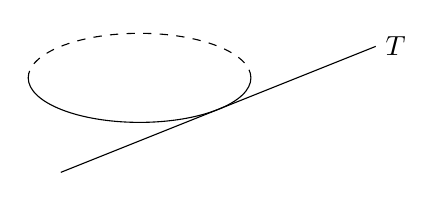
\begin{tikzpicture}[yscale=.4]
\draw[dashed](0.414,1) arc (0:180:1.414);
\draw(0.414,1) arc (0:-180:1.414);
\tkzDefPoints{0.414/1/B, -2.414/1/C, -1/9/V, 0/0/A,-1/1/O}
\draw(2,2)node[right]{$T$}--(-2,-2);
\tkzDrawSegments(V,C V,A V,B)
\tkzDrawSegments[dashed](V,O O,A)
\tkzLabelPoints[above](V)
\tkzLabelPoints[left](C,O)
\tkzLabelPoints[below right](A)
\tkzLabelPoints[right](B)
\end{tikzpicture}
    \caption{}
\end{figure}

求证:$AT\bot VA$
\end{example}

\begin{proof}
设$O$为圆锥底面的圆心,连接
$VO$、$OA$, 则$VO\bot$平面$ABC$.

$\therefore\quad VA$在平面$ABC$上的射影是$OA$.

$\because\quad AT$是$\odot O$的切线,

$\therefore\quad OA\bot AT$

由三垂线定理,有$AT\bot VA$.
\end{proof}

\begin{ex}
\begin{enumerate}
    \item \begin{enumerate}
        \item 底面是正多边形的棱锥是正棱锥吗?
    \item 侧棱都相等的棱锥是正棱锥吗?
    \item 侧面和底面夹角都相等的棱锥是正棱锥吗?
    \end{enumerate}
  
    \item 
    \begin{enumerate}
      \item 棱锥的侧棱和底面所成的角都相等,则顶点在底面
    上的射影是什么?
    \item 棱锥的侧面和底面所成的二面角都相等,则顶点在
    底面上的射影是什么?  
    \end{enumerate}
    
    \item 证明:六条棱长相等三棱锥是正三棱锥.
    \item 试用两种画法分别画出底面边长为6cm, 高为15cm的
    正六棱锥的直观图,比例尺为
    \item 用第二种画法画出底面半径是2cm, 母线为3cm的圆锥的
    直观图.
    \item 用第一种画法画出底面边长为2cm, 高为4cm的正五棱
    的直观图.
    \item 在正六棱锥$V-ABCDEF$中,底面多边形的边长为$a$,
    侧棱长为$2a$, 求这棱锥的高$VO$及斜高$VM$的长.
    \item 已知圆锥底面圆的半径为3cm, 高为4cm, 设$VA$是圆锥
    的一条母线,$O$点是底面中心,如果$OM\bot VA$于$M$, 求
    $OM$的长.
\end{enumerate}
\end{ex}

\subsection{台体}
\begin{blk}{定义}
    平行于棱锥底面的平面与棱锥侧面相截,棱锥在
底面和截面之间的部分叫做棱台.原棱锥的底面和截面叫做
棱台的下底面和上底面,其他各面叫侧面,两相邻侧面的公
共边叫做棱台的侧棱,两个底面之间的距离叫做棱台的高.
(图2.20)
\end{blk}

\begin{figure}[htp]
    \centering
\begin{tikzpicture}[scale=1.3]
\begin{scope}
    \tkzDefPoints{0/0/A, 2/0/B, 2.75/.75/C, .75/.75/D, 1.375/3/S, 1.375/.375/O}
    \tkzDefMidPoint(S,A) \tkzGetPoint{A'}
    \tkzDefMidPoint(S,B) \tkzGetPoint{B'}
    \tkzDefMidPoint(S,C) \tkzGetPoint{C'}
    \tkzDefMidPoint(S,D) \tkzGetPoint{D'}
    \tkzDefMidPoint(S,O) \tkzGetPoint{O'}
    \tkzDrawPolygon(A',B',C',D')
    \tkzDrawSegments(A,B B,C A,A' B,B' C,C')
    \tkzDrawSegments[dashed](A',S B',S C',S O,S A,D C,D S,D)
    \tkzLabelPoints[below](A,B)
    \tkzLabelPoints[left](A',D',D)
    \tkzLabelPoints[right](C,C',B',O,O')

\node at (1.5,-.5){(1)};
\end{scope}
\begin{scope}[xshift=5cm]
    \tkzDefPoints{0/0/A, 2/0/B, 2.75/.75/C, .75/.75/D, 1.375/3/S, 1.375/.375/O}
\tkzDefMidPoint(S,A) \tkzGetPoint{A'}
\tkzDefMidPoint(S,B) \tkzGetPoint{B'}
\tkzDefMidPoint(S,C) \tkzGetPoint{C'}
\tkzDefMidPoint(S,D) \tkzGetPoint{D'}
\tkzDrawPolygon(A',B',C',D')
\tkzDrawSegments(A,B B,C A,A' B,B' C,C')
\tkzDrawSegments[dashed](A,D C,D D',D)
\node at (1.5,-.5){(2)};
\end{scope}
\end{tikzpicture}
    \caption{}
\end{figure}


棱台可以用表示上、下底顶点的字母来表示,例如棱台
$AC'$. 也可记作棱台$ABCD-A'B'C'D'$(图2.20(1)).

由三棱锥、四棱锥、五棱锥……截得的棱台分别叫做\textbf{三
棱台、四棱台、五棱台}……

\begin{blk}
{定义} 由正棱锥截得的棱台叫做正棱台.    
\end{blk}



\begin{figure}[htp]
    \centering
\begin{tikzpicture}[scale=1.3]
\begin{scope}
    \tkzDefPoints{-.5/0/A, .5/0/B, -1.1/.4/E, 1.1/.4/C, 0/.8/D, 0/2.5/S}
    \tkzDefMidPoint(S,A) \tkzGetPoint{A'}
    \tkzDefMidPoint(S,B) \tkzGetPoint{B'}
    \tkzDefMidPoint(S,C) \tkzGetPoint{C'}
    \tkzDefMidPoint(S,D) \tkzGetPoint{D'}
    \tkzDefMidPoint(S,E) \tkzGetPoint{E'}
    \tkzDrawPolygon(A',B',C',D',E')
    \tkzDrawSegments(A,B B,C E,A A,A' B,B' C,C' E,E')
    \tkzDrawSegments[dashed](A',S S,E'  B',S C',S  C,D E,D)
    
    \node at (0,-.5){(1)};

\end{scope}
\begin{scope}[xshift=3cm]
    \tkzDefPoints{0/0/A, 2/0/B, 2.75/.75/C, .75/.75/D, 1.375/3/S, 1.375/.375/O, 2.375/.375/E}
\tkzDefMidPoint(S,A) \tkzGetPoint{A'}
\tkzDefMidPoint(S,B) \tkzGetPoint{B'}
\tkzDefMidPoint(S,C) \tkzGetPoint{C'}
\tkzDefMidPoint(S,D) \tkzGetPoint{D'}
\tkzDefMidPoint(S,E) \tkzGetPoint{E'}
\tkzDefMidPoint(S,O) \tkzGetPoint{O'}
\tkzDrawPolygon(A',B',C',D')
\tkzDrawSegments(A,B B,C A,A' B,B' C,C' E,E')
\tkzDrawSegments[dashed](A,D C,D D',D O,O' O,E O',E' O,B O',B')
\node at (1.5,-.5){(2)};
\end{scope}
\end{tikzpicture}
    \caption{}
\end{figure}

正棱台有下面一些性质:
\begin{enumerate}
\item 正棱台的两个底面及平行于底面的截面是相似的正
多边形.(图2.21)
\item 两底面中心连线垂直于底面(图2.21(2)).
\item 正棱台的各侧面是全等的等腰梯形,各等腰梯形的
高相等,它叫做正棱台的斜高.(图2.21(2))
\item 正棱台的各侧棱相等,并且延长后相交于一点.
(图2.21(1))
\item 正棱台两底面中心连线、相应的两底面的边心距和
斜高组成直角梯形;两底中心连线、侧棱和两底面相应的半
径组成一个直角梯形;同一个侧面上的上底和下底中点的连
线将这个侧面分成两个全等的直角梯形.(见图2.21(2))
\end{enumerate}

解正棱台的问题一般总可化为解5中提到的直角梯形
及底面的正多边形的问题.

\begin{example}
    设正三棱台的两个底面边长分别是2cm和5cm, 侧
棱长为5cm, 求这个棱台的高和斜高(图2.22).
\end{example}

\begin{figure}[htp]
    \centering
\begin{tikzpicture}[scale=1.2]
\tkzDefPoints{0/0/A, 4/0/C, 3/-1.5/B, 2.5/3/S, 2.5/-.45/O, 1.5/-.75/D}
\tkzDefMidPoint(S,A) \tkzGetPoint{A_1}
\tkzDefMidPoint(S,B) \tkzGetPoint{B_1}
\tkzDefMidPoint(S,C) \tkzGetPoint{C_1}
\tkzDefMidPoint(S,O) \tkzGetPoint{O_1}
\tkzDefMidPoint(S,D) \tkzGetPoint{D_1}

\tkzDrawPolygon(A_1,B_1,C_1)
\tkzDrawSegments(A,B B,C A,A_1 B,B_1 C,C_1 A_1,O_1 O_1,D_1 D_1,D)
\tkzDrawSegments[dashed](O,D A,C A,O O,O_1)

\tkzLabelPoints[left](A,A_1,D_1)
\tkzLabelPoints[right](C,C_1,O,O_1,B_1)
\tkzLabelPoints[below](B,D)
\tkzDefPointsBy[translation = from O_1 to D_1](O){F}
\tkzDefPointsBy[translation = from O_1 to A_1](O){E}
\tkzDrawSegments[dashed](D_1,F A_1,E)
\tkzLabelPoints[below](E,F)



\end{tikzpicture}
    \caption{}
\end{figure}


\begin{solution}
设两底面的中心分别为$O_1$和$O$, 连接$O_1O$, $O_1A_1$,
 $OA$. 取$A_1B_1$的中点$D_1$, $AB$的中
点$D$, 连接$O_1D_1$, $OD$, $D_1D$. 则
$O_1O$是棱台的高,$DD_1$是棱台的
斜高;并知$O_1A_1AO$和$OO_1D_1D$是两个直角梯形.分别引$A_1E\bot
AO$于$E$, $D_1F\bot DO$于$F$. 

由于上、下两底的边长分
别为2cm和5cm.

因此:
\[O_1A_1=\frac{\sqrt{3}}{3}\x 2=\frac{2}{3}\sqrt{3}, \qquad  OA=\frac{\sqrt{3}}{3}\x 5=\frac{5}{3}\sqrt{3}\]
因此:$AE=OA-O_1A_1=\frac{5}{3}\sqrt{3}-\frac{2}{3}\sqrt{3}=\sqrt{3}$


在直角$\triangle AA_1E$中,
\[A_1E=A_1A_2-AE_2=\sqrt{5^2-(\sqrt{3})^2}=\sqrt{22}\approx 4.69\]

$\therefore\quad OO_1=A_1E=\sqrt{22}\approx 4.69$(cm)

又$\because\quad O_1D_1=\frac{\sqrt{3}}{6}\x 2=\frac{\sqrt{3}}{3},\qquad OD=\frac{\sqrt{3}}{6}\x 5=\frac{5}{6}{\sqrt{3}}$

$\therefore\quad DF=OD-O_1D_1=\frac{5}{6}{\sqrt{3}}-\frac{\sqrt{3}}{3}=\frac{\sqrt{3}}{2}$

在直角$\triangle DD_1F$中
\[\begin{split}
    D_1D&=\sqrt{DF^2+D_1F^2}=\sqrt{DF^2+O_1O^2}\\
&=\sqrt{\left(\frac{\sqrt{3}}{2}\right)^2+(\sqrt{22})^2}=\frac{1}{2}\sqrt{91}\approx 4.77({\rm cm})
\end{split}\]

答:这棱台的高约等于4.69cm, 斜高约等于4.77cm.
\end{solution}

\begin{blk}
    {定义} 平行于圆锥底面的平面与圆锥相截,圆锥的底面
和截面之间的部分叫做圆台.原来圆锥的底面和截面分别叫
做圆台的下底面和上底面,原来圆锥的轴叫做圆台的轴,原
来圆锥的母线夹在两底面之间的部分叫做圆台的母线,原来
圆锥的侧面夹在两底面之间的部分叫做圆台的侧面,两底面
之间的距离叫做圆台的高.(图2.23)
\end{blk}

圆台也可以看作是一个直角梯形绕着垂直于底边的一条
腰所在的直线为轴,旋转$360^{\circ}$时,这个直角梯形的两底边及
另一腰所形成的面围成的几何体.直角梯形的上、下两底边旋
转而成的圆面分别叫做圆台的上底面和下底面.直角梯形垂
直于底边的腰的长叫做圆台的高,而另一腰则称为圆台的母
线.(图2.24)

\begin{figure}[htp]\centering
    \begin{minipage}[t]{0.48\textwidth}
    \centering
\begin{tikzpicture}[>=latex, yscale=.4]
\tkzDefPoints{-1.5/0/A_1, 1.5/0/C_1, -1/4/A, 1/4/C, 0/0/O_1, 0/4/O, 0/12/S}
\tkzDefPoint(-120:1.5){B_1}
\draw(O) circle (1);
\draw(C_1) arc (0:-180:1.5);
\draw(C_1)[dashed] arc (0:180:1.5);
\tkzDrawSegments(A,A_1 C,C_1)
\tkzDrawSegments[dashed](A,S C,S S,O_1 S,B_1)
\tkzLabelPoints[left](A,A_1)
\tkzLabelPoints[right](C,C_1,O,O_1)
\tkzLabelPoints[below](B_1)
\tkzInterLC(S,B_1)(A,C) \tkzGetPoints{B'}{B}
\tkzDrawLines[add=0 and .3](B_1,B) \tkzLabelPoints[right](B)
\tkzLabelPoints[above](S)
    \end{tikzpicture}
    \caption{}
    \end{minipage}
    \begin{minipage}[t]{0.48\textwidth}
    \centering
    \begin{tikzpicture}[>=latex, yscale=.4]
        \tkzDefPoints{-1.5/0/A_1, 1.5/0/C_1, -1/4/A, 1/4/C, 0/0/O_1, 0/4/O, 0/12/S}
        \tkzDefPoint(-120:1.5){B_1}
\draw(O) circle (1);
\draw(C_1) arc (0:-180:1.5);
\draw(C_1)[dashed] arc (0:180:1.5);
\tkzDrawSegments(A,A_1 C,C_1)
\tkzDrawSegments[dashed](O,O_1 O_1,C_1)
\tkzDrawSegments(C_1,C O,C) 
\tkzLabelPoints[left](O, O_1)
\node at (C)[right]{$A$};
\node at (C_1)[right]{$B$};
\node at (.5,4)[above]{$R_1$};
\node at (.75,0)[above]{$R_2$};
    \end{tikzpicture}
    \caption{}
    \end{minipage}
    \end{figure}


圆台的表示法是用它两底上而不在同一条母线上的两个
点的字母来表示.如图2.23的圆台可以记作圆台$AB_1$.

圆台有下面一些性质:
\begin{enumerate}
\item 圆台的两个底面是圆,它们所在的平面平行.
\item 圆台的轴经过两个底面的圆心,并且和底面垂直,
连结两底圆心线段的长等于高.
\item 圆台的母线都相等.
\item 圆台的各母线的延长线交于一点.
\item 经过圆台的轴的截面叫圆台的轴截面,它是一个等
腰梯形.
\item 经过圆台的轴的平面是圆台的对称平面.
\end{enumerate}

如果设圆台的上、下两底面的半径分别为$R_1$和$R_2$, 母线
长为$\ell$, 高为$h$, 那么$\ell^2=(R_2-R_1)^2+h^2$ (图2.24)

\begin{example}
    已知一个圆台两底面面积分别是$1{\rm dm^2}$和$49{\rm dm^2}$, 有
    一个截面和底面平行,它的面积是$25{\rm dm^2}$, 求这个截面和两
    个底面距离的比.
\end{example}

\begin{figure}[htp]
    \centering
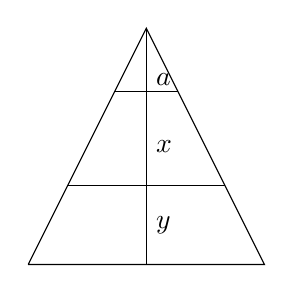
\begin{tikzpicture}[scale=.5]
\draw(-3,0)--(3,0)--(0,6)--(-3,0);
\draw(-2,2)--(2,2);
\draw(-1+.2,4+.4)--(1-.2,4+.4);
\draw(0,0)--(0,6);
\node at (0,1) [right]{$y$};
\node at (0,3) [right]{$x$};
\node at (0,4.7) [right]{$a$};
\end{tikzpicture}
    \caption{}
\end{figure}

\begin{solution}
    设从截得圆台的原来圆锥的顶点到圆台上底的距离
是$a$ $(a>0)$, 从截面到圆台上底面和下底
面的距离分别是$x$和$y$, 那么参看轴截面
图2.25,由圆台的性质及相似形面积的比等于相似比的平方,就得到
\[\frac{(a+x)^2}{a^2}=\frac{25}{1},\qquad \frac{(a+x+y)^2}{a^2}=\frac{49}{1}\]
由此得正数解$x=4a$, $y=2a$.因此,$x:y=4a:2a=2:1$

答:截面和上、下两底面距离的比为2:1.
\end{solution}



\begin{ex}
\begin{enumerate}
    \item 如果两个相似三角形(不在同一平面内)的对应边互相
    平行,连结它们的对应顶点而形成各面所围成的几何体
    是不是棱台.
    \item 已知正棱台上、下两底面的边长分别是$a$和$b$ $(a<b)$, 侧
    棱和底面成$45^{\circ}$角,求它的侧棱和斜高的长.
    \item 圆台的两底面半径分别是$r_1$和$r_2$ ($r_1>r_2$), 母线与底面夹
    角是$60^{\circ}$, 求它的高.
    \item 圆台的母线长为$2a$, 母线与轴的夹角为$30^{\circ}$,一个底面半径是另一个底面半径的2倍,求两底面的半径.
    \item 下图是正四棱台的二视图,
    (图中所标尺寸单位是cm)
    试用两种画法画出它的直观
    图,比例尺为
    1/3.
\end{enumerate}
\end{ex}

\begin{figure}[htp]
    \centering
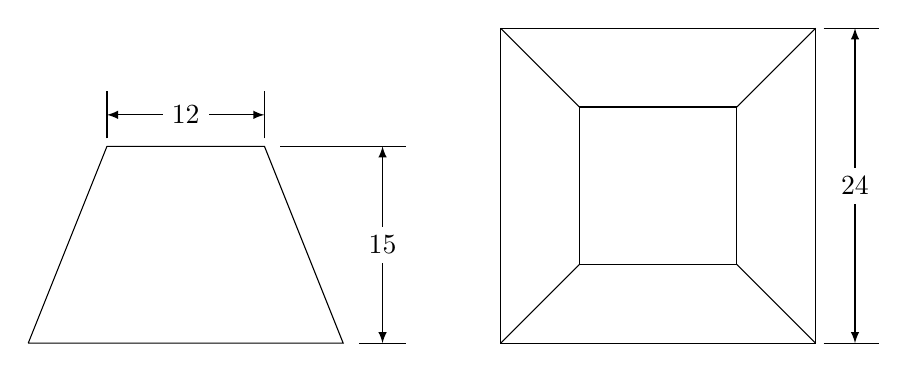
\begin{tikzpicture}[>=latex]
\begin{scope}
\draw(0,0)--(4,0)--(3,2.5)--(1,2.5)--(0,0);
\draw[<->](3,2.9)--node[fill=white]{12}(1,2.9);
\draw[<->](4.5,0)--node[fill=white]{15}(4.5,2.5);
\draw(4.2,0)--(4.8,0);
\draw(3.2,2.5)--(4.8,2.5);
\draw(1,2.6)--(1,3.2);
\draw(3,2.6)--(3,3.2);
\end{scope}
\begin{scope}[xshift=6cm]
\draw(0,0) rectangle(4,4);
\draw(1,1) rectangle(3,3);
\draw[<->](4.5,0)--node[fill=white]{24}(4.5,4);
\draw(1,1)--(0,0);
\draw(3,3)--(4,4);\draw(3,1)--(4,0);
\draw(1,3)--(0,4);
\draw(4.1,0)--(4.8,0);
\draw(4.1,4)--(4.8,4);
\end{scope}
\end{tikzpicture}
    \caption*{第5题}
\end{figure}

\subsection{球}

\begin{blk}
    {定义} 在空间与定点距离相
的点的集合称做球面.球面所
包围的立体叫做球.定点叫做球
心,定点和球面上任一点所连线
段叫做球的半径.连结球面上任意两点的线段叫做球的弦,
通过球心的弦叫做球的直径.
\end{blk}

球面也可以看作半圆绕着它的直径旋转一周所成的图
形.球可以看作是一半圆面绕着它的直径旋转一周而形成的
立体.原半圆面的半径是球的半径,原半圆面的圆心是球
心.

一个球可以用表示它球心的字母来表示,例如“球$O$”.
画半径是$R$的直观图时,一般用第二种画法,先分别在$XOY$、
$XOZ$、$YOZ$三个平面的画出表示半径是$R$的圆的三个椭圆,再
在外面画一个圆和这三个椭圆相切(图2.26),通常用简便
的画法如图2.27.

\begin{figure}[htp]\centering
    \begin{minipage}[t]{0.48\textwidth}
    \centering
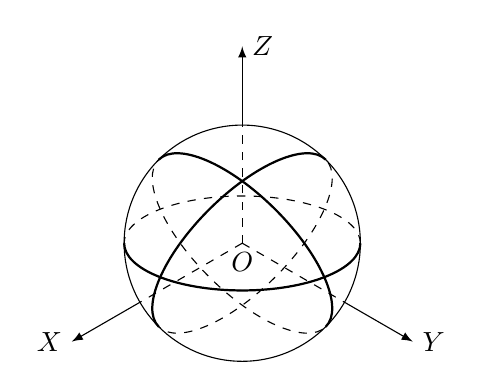
\begin{tikzpicture}[>=latex, scale=1]
\draw(0,0) circle(1.5);
\foreach \x in {90,-30,-150}
{
    \draw[dashed](0,0)--(\x:1.5);
    \draw[->](\x:1.5)--(\x:2.5);
}

\node at (90:2.5)[right]{$Z$};
\node at (-30:2.5)[right]{$Y$};
\node at (-150:2.5)[left]{$X$};
\node at (0,0)[below]{$O$};
\draw[dashed](0,0) ellipse [x radius=1.5, y radius= .6, rotate=45];
\draw[dashed](0,0) ellipse [x radius=1.5, y radius= .6, rotate=-45];
\draw[dashed](0,0) ellipse [x radius=1.5, y radius= .6];
\draw[thick](-1.5,0) arc [x radius=1.5, y radius= .6, start angle=180, delta angle=180];
\draw[thick, rotate=45](-1.5,0) arc [x radius=1.5, y radius= .6, start angle=180, delta angle=-180];
\draw[thick, rotate=-45](-1.5,0) arc [x radius=1.5, y radius= .6, start angle=180, delta angle=-180];
    \end{tikzpicture}
    \caption{}
    \end{minipage}
    \begin{minipage}[t]{0.48\textwidth}
    \centering
    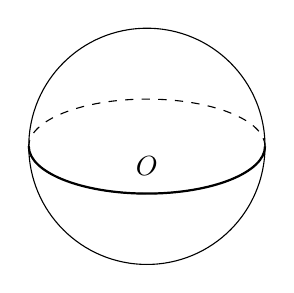
\begin{tikzpicture}[>=latex, scale=1]
        \draw(0,0) circle(1.5);  
        \draw[dashed](0,0) ellipse [x radius=1.5, y radius= .6];
        \draw[thick](-1.5,0) arc [x radius=1.5, y radius= .6, start angle=180, delta angle=180];
        \node at (0,0)[below]{$O$};
        \tkzDrawPoint(0,0)
    \end{tikzpicture}
    \caption{}
    \end{minipage}
    \end{figure}



球有下列一些性质:
\begin{enumerate}
    \item 同球的半径(或直径)相等.
    \item 球被平面所截得截面是一圆面.
\end{enumerate}

\begin{figure}[htp]
    \centering
\begin{tikzpicture}[>=latex]
\begin{scope}
    \tkzDefPoints{0/0/O, 1.5/0/M, -1.5/0/N}
    \draw[dashed] (O) ellipse [x radius=1.5, y radius=.8];
    \draw[thick] (M) arc [x radius=1.5, y radius=.8, start angle =0, end angle =-180];
\tkzLabelPoints[above](O)
\tkzDefPoints{-2.5/-1/a, 2.5/-1/b, 3/1/c}
\tkzDefPointsBy[translation= from b to c](a){d}
\tkzLabelPoint[above right](a){$M$}
\tkzInterLC(a,b)(O,M)
\tkzGetPoints{T1}{T2}
\tkzDrawArc[color=black, thick](O,M)(N)
\tkzDrawArc[color=black, dashed](O,M)(T2)
\tkzDrawArc[color=black, dashed](O,T1)(N)
\tkzDrawArc[color=black, thick](O,T2)(T1)
\tkzDefPoints{-1/-.5/A, 1/-.5/B}
\tkzDrawSegments[dashed](O,A O,B)
\tkzLabelPoints[above](A,B)
\tkzInterLC(c,d)(O,M)
\tkzGetPoints{T3}{T4}
\tkzDrawSegments(a,b b,c d,a)
\tkzDrawSegments[dashed](T3,T4)
\tkzDrawSegments(d,T3 T4,c)
\node at (0,-2){(1)};
\end{scope}
\begin{scope}[xshift=6cm]
    \tkzDefPoints{0/0/O, 1.3/-.75/M, 0/-.75/O_1, -1.3/-.75/N'}
    \draw[dashed] (O_1) ellipse [x radius=1.3, y radius=.35];
    \draw[thick] (M) arc [x radius=1.3, y radius=.35, start angle =0, end angle =-180];
\tkzLabelPoints[above](O)
\tkzDefPoints{-2.5/-1.25/a, 2.5/-1.25/b, 3/.75/c}
\tkzDefPointsBy[translation= from b to c](a){d}
\tkzDrawSegments(a,b b,c d,a)
\tkzLabelPoint[above right](a){$M$}
\tkzInterLC(a,b)(O,M)
\tkzGetPoints{T1}{T2}
\tkzInterLC(c,d)(O,M)
\tkzGetPoints{T3}{T4}
\tkzDrawArc[color=black, thick](O,M)(N')
\tkzDrawArc[color=black, dashed](O,M)(T2)
\tkzDrawArc[color=black, dashed](O,T1)(N)
\tkzDrawSegments[dashed](T3,T4)
\tkzDrawSegments(d,T3 T4,c)
\tkzDrawArc[color=black, thick](O,T2)(T1)

\node at (0,-2){(2)};
    
\tkzDefPoints{-.9/-1/A, .9/-1/B}
\tkzDrawSegments[dashed](O,A O,B O_1,A O_1,B O,O_1)
\tkzLabelPoints[above](A,B)
\tkzLabelPoints[below](O_1)


\end{scope}
\end{tikzpicture}  
    \caption{}
\end{figure}

\begin{proof}
    设平面$M$通过球心$O$, 并设$A$、$B$为平面$M$和球面交线
    上任意两点.(图2.28(1))在平面$M$内连接$OA$, $OB$, 因
    $OA$、$OB$都是球$O$的半径,所以$OA=OB$. 这就是说,交线上
    任意两点,因为交线上一切点与$O$点等距离,所以交线是平
    面$M$内以$O$点为圆心的一个圆,它的半径就等于球的半径,
    因此球$O$与平面$M$的截面是以球心为圆心的圆面.

设平面$M$不通过球心(图2.28(2)),自球心$O$作$OO_1$
    垂直平面$M$于$O_1$, 设$A$、$B$为平面$M$与球$O$的交线上任意两点,
    连结$OA$, $OB$, 因为$OA=OB$, 所以它们在平面$M$内的射影相
    等,即$AO_1=BO_1$, 因此平面$M$与球$O$的交线是一个圆,它的圆
    心就是球心$O$到平面的垂线的垂足$O_1$. 如果用$R,r$分别表示球
    的半径和截面圆的半径,$d$表示由球心$O$到平面$M$的距离,
那么,
\[r=\sqrt{R^2-d^2}\]
因此,平面$M$和球$O$的截面是以$O_1$为圆心,以$\sqrt{R^2-d^2}$
为半径的圆面.
\end{proof}

\begin{blk}{推论}
\begin{enumerate}
\item 连结球心与截面圆的圆心的直线和截面垂直.
\item 与球心距离相等的截面的圆大小相等.
\item 与球心距离不等的截面,所截得的圆的大小不等,距
离球心较近的截面所截的圆较大.
\item 当$d=0$时,这时截面过球心,所以$r=R$, 也就是说,
这时截面的圆的半径最大,称这个圆为球的大圆,不过球心
截面的圆称为球的小圆.
\item 当$d=R$时,$r=0$, 这时截面的圆退化为一个点,我们
称和球面只有一个公共点的乎面叫做球的切面,球的切面和
球的公共点叫做切点.和球只有一个公共点的直线叫做球的
切线.显然在球的切面上过切点的直线是球的切线.
\end{enumerate}
    
\end{blk}

\begin{blk}{定义} 
    连结球面上$A$、$B$两点间大圆的劣孤叫做球面上
$A$、$B$两点间的球面距离.
\end{blk}

\begin{blk}
    {定理} 如果球的半径通过球面
    的切面的切点,这个半径必垂直于
    球的切面.
\end{blk}

\begin{figure}[htp]
    \centering
\begin{tikzpicture}[>=latex]
    \tkzDefPoints{0/0/O, 2/0/M}
    \draw[dashed] (O) ellipse [x radius=2, y radius=.8];
    \draw[thick] (M) arc [x radius=2, y radius=.8, start angle =0, end angle =-180];
\tkzLabelPoints[below](O)
\tkzDefPoints{-2.5/1.5/a, 2.5/1.5/b, 3/2.5/c}
\tkzDefPointsBy[translation= from b to c](a){d}
\tkzDrawPolygon(a,b,c,d)
\tkzInterLC(a,b)(O,M) \tkzGetPoints{t1}{t2}
\tkzDrawArc[thick, color=black](O,t1)(t2)
\tkzDrawArc[dashed, color=black](O,t2)(t1)
\tkzLabelPoint[above right](a){$\alpha$}
\tkzDefPoints{0/1.8/K, .75/1.75/K'}
\tkzLabelPoints[left](K',K)
\tkzDrawSegments[dashed](O,K O,K')
\tkzDrawPoints(K',K)

\end{tikzpicture}   
    \caption{}
\end{figure}

\begin{proof}
    设平面$\alpha$是球$O$的切面,
    $K$点是切点,$KO=R$, (图2.29)
    如果$OK$不垂直平面$\alpha$, 作$OK'\bot$
    平面$\alpha$于$K'$, 则$OK>OK'$, 即$R>OK'$, $K'$点在球面的内部,这样,平面$\alpha$与球$O$必相交,这
与$\alpha$是球$O$的切面相矛盾,所以$OK\bot\alpha$.
\end{proof}

\begin{blk}
  {逆定理} 垂直于球半径且过半径外瑞的平面必是球的切
面.  
\end{blk}

\begin{proof}
在平面$\alpha$上另取任一点$K'$, 连结$OK'$, 因为$OK$是
平面$\alpha$的垂线,而$OK'$是平面$\alpha$的斜线,所以$OK'>OK$· 
因为$K\in\alpha$, 所以$K'$点在球面外,也就是说,平面$\alpha$上除$K$点外的任何点都不在球面上,即平面$\alpha$与球面只有一个公共
点$K$, 所以平面$\alpha$是球$O$的切面.
\end{proof}

把上面正、逆定理合成一个定理,即

\begin{blk}
    {定理} 一个平面是一个球的切面的充要条件是这个平面
经过这个球的一条半径的外端而且和这条半径垂直.
\end{blk}

综上所述,可知,如果球的半径为$R$, 球心$O$到平面的距
离为$d$, 则平面$\alpha$与球$O$有下列位置关系:
\begin{enumerate}
\item 如果$d<R$, 那么平面$\alpha$与球$O$相交,截面是个圆,
它的半径$r=\sqrt{R^2-d^2}$
\item 如果$d=R$, 那么平面$\alpha$与球$O$相切.
\item 如果$d>R$, 那么平面$\alpha$与球$O$没有公共点,这时
称平面$\alpha$与球$O$相离.
\end{enumerate}

\begin{example}
    设$A$地位于北纬$45^{\circ}$, 由
于地球自转,在一小时内$A$点转了多少路程?(地球的半径大约为6370公
里)
\end{example}


\begin{solution}
    如图2.30, 设点$O$是地球的
    球心,$OA$是地球的半径,$M$是北纬
    $45^{\circ}$圈的中心,$AM$是北纬$45^{\circ}$圈的半
    径,$OM$是地球球心到北纬$45^{\circ}$圈所在平面的距离,那么
在直角$\triangle AMO$中,
$\angle OAM=\angle AOB=45^{\circ}$

$\therefore\quad AM=AO\cos45^{\circ}\approx 6370\x0.7071\approx 4504$

因为地球自转一周的时间为24小时,所以地球自转一小
时转过的角度为$\frac{2\pi}{24}=\frac{\pi}{12}$(弧度),于是,$A$地在一小时内转
过的路程即为北纬$45^{\circ}$圈的$\frac{\pi}{12}$弧度的弧长,即
\[\frac{\pi}{12}\x 4504\approx \frac{3.1416}{12}\x 4504\approx 1179\]

答:$A$地在一小时内转过的路程约为1179公里.
\end{solution}

\begin{figure}[htp]\centering
    \begin{minipage}[t]{0.48\textwidth}
    \centering
  \begin{tikzpicture}[>=latex, scale=1]
    \tkzDefPoints{0/0/O, 2/0/B, 0/1.414/M}
    \tkzDefPoint(45:2){A}
    \tkzDrawCircle(O,A)
    \tkzDrawSegments[dashed](A,M M,O O,B O,A)
    \tkzMarkAngle[mark=none, size=.4](B,O,A)    
    \tkzLabelAngle[pos=.7](B,O,A){$45^{\circ}$}    
    \draw[dashed] (O) ellipse [x radius=2, y radius=.5];
    \draw[dashed] (M) ellipse [x radius=1.414, y radius=.25];
    \tkzLabelPoints[right](A,B)
    \tkzLabelPoints[left](M,O)
    \draw[thick] (B) arc [x radius=2, y radius=.5, start angle =0, end angle =-180];
    \draw[thick] (A) arc [x radius=1.414, y radius=.25, start angle =0, end angle =-180];
    
    \end{tikzpicture}
    \caption{}
    \end{minipage}
    \begin{minipage}[t]{0.48\textwidth}
    \centering
    \begin{tikzpicture}[>=latex, scale=1]
      \tkzDefPoints{0/0/O, 2/0/M}
    \tkzDrawCircle(O,M)
    \draw[dashed] (O) ellipse [x radius=2, y radius=.8];
    \draw[thick] (M) arc [x radius=2, y radius=.8, start angle =0, end angle =-180];
\tkzDefPoints{-1.2/-.62/A, .5/-.75/B}
\tkzDrawPoints(A,B)
\tkzLabelPoints[below](A,B)
\tkzLabelPoints[above](O)
\tkzMarkAngle[mark=none, size=.3](A,O,B)    
\tkzLabelAngle[pos=.6](A,O,B){$50^{\circ}$}  
\tkzDrawSegments[dashed](O,A O,B)
    \end{tikzpicture}
    \caption{}
    \end{minipage}
    \end{figure}

\begin{example}
    已知球面上$A$、$B$两点的球面距离为$5\pi$cm, 过这
两点的半径的夹角$\angle AOB$是50度,求这个球的半径.
\end{example}


\begin{solution}
    如图2.31, $O$为球心,过半径
$OA$和$OB$作平面,则这个平面所截
的圆为大圆,在这个圆上已知圆心角
$\angle AOB=50^{\circ}$, $AB=5\pi$cm. 设球的半
径为$R$, 则
\[5\pi=\left(\frac{50\pi}{180}\right)\cdot R\quad \Rightarrow\quad R=18\]

答:这个球的半径为18cm.
\end{solution}

\begin{ex}
\begin{enumerate}
    \item 求证:经过球上同一个切点的所有切线的集合是球的切
    面.
    \item 求证:两球相交的交线是一个圆.
    \item 求证:一动点与两个定点的距离的平方和为一个常数,
    则动点的轨迹是一个球.
    \item 试证:球面任意三点$A$、$B$、$C$都不可能共线.
    \item 
    首都北京位于北纬$40^{\circ}$, 已知地球半径约为6370公里,
    求首都所在的纬度圈半径.(精确到10公里)
\end{enumerate}
\end{ex}

\subsection{多面体和旋转体}
\begin{blk}
{定义} 由几个多边形\footnote{注:这里所说的多边形包括它内部的平面部分.}围成的封闭的几何体叫多面体.
围成多面体的各个多边形叫做多面体的面,各相邻面的公共
边叫多面体的棱,相交于同一顶点的侧面组成一个多面角,
各多面角的顶点叫做多面体的顶点.不在同一个面内的两个
顶点的连线叫做多面体的对角线.图2.32的各图表示的都是
多面体.    
\end{blk}

\begin{figure}[htp]
    \centering
\begin{tikzpicture}
\begin{scope}
\tkzDefPoints{0/.5/A, 1/-.1/B, 3/.5/C, 1.3/1/D}
\tkzDefPoints{0.75/2.5/A', 1.4/1.8/B', 2.2/1.9/C', 2.6/2.5/D'}
\tkzDrawPolygon(A',B',C',D')
\tkzDrawSegments(A,A' B,B' C',C C,D' A,B B,C)
\tkzDrawSegments[dashed](D,C D,A D,D' D,A')
\node at (1,-.5){(1)};
\end{scope}
\begin{scope}[xshift=4cm]
\tkzDefPoints{0/0/A, 2/0/B, 2/2/C, 0/2/D, .75/.75/A'}
\tkzDefPointsBy[translation= from A to A'](B,C,D){B',C',D'}
\tkzDrawPolygon(D,C',B)
\tkzDrawPolygon(A,D,D',C',B',B)
\tkzDrawSegments[dashed](A',B' A',A A',D')
\node at (1,-.5){(2)};
\end{scope}
\begin{scope}[xshift=8cm]
    \tkzDefPoints{0/0/A, 3/0/B, 3/1.5/C, 0/1.5/D, .75/.75/A'}
    \tkzDefPointsBy[translation= from A to A'](B,C,D){B',C',D'}
    \tkzDrawPolygon(A,B,C,D)
    \tkzDrawSegments[dashed](A',B' A',A A',D')
    \tkzDrawSegments(B,B' C',C D,D' C',D' C',B')
    \node at (1.5,-.5){(3)};
\end{scope}
\end{tikzpicture}
    \caption{}
\end{figure}

前面讲过的棱柱、棱锥、棱台都是多面体.

\begin{blk}
    {定义} 使平面内的曲线(也包括直线在内),围绕这个
平面里的一条直线旋转一周,回到原来位置这时所成的曲面
叫旋转面,由旋转面围成的几何体叫转旋体.前面讲过的
圆柱、圆锥、圆台和球分别是由矩形、直角三角形、直角梯
形和半圆以一条直角边(或直径)所在直线为轴,旋转一周
而形成的旋转体(图2.33).
\end{blk}

\begin{figure}[htp]
    \centering
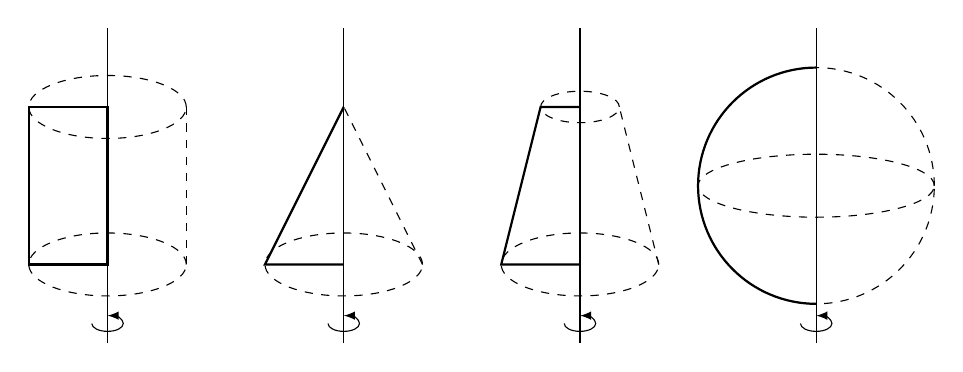
\begin{tikzpicture}[>=latex]
\begin{scope}
\draw(0,0)--(0,4);
\draw[dashed](0,1) ellipse[x radius=1, y radius=.4];
\draw[dashed](0,3) ellipse[x radius=1, y radius=.4];
\draw[thick](0,1) rectangle (-1,3);
\draw[dashed](1,1)--(1,3);
\draw[->](-.2,0.25) arc [x radius=.2, y radius=.1, start angle =180, end angle =180+270];
\end{scope}
\begin{scope}[xshift=3cm]
    \draw(0,0)--(0,4);
\draw[dashed](0,1) ellipse[x radius=1, y radius=.4];
\draw[thick](0,1)--(-1,1)--(0,3);
\draw[dashed](1,1)--(0,3);
\draw[->](-.2,0.25) arc [x radius=.2, y radius=.1, start angle =180, end angle =180+270];
\end{scope}
\begin{scope}[xshift=6cm]
    \draw(0,0)--(0,4);
\draw[dashed](0,1) ellipse[x radius=1, y radius=.4];
\draw[dashed](0,3) ellipse[x radius=.5, y radius=.2];
\draw[thick](0,1)--(-1,1)--(-.5,3)-- (0,3);
\draw[dashed](1,1)--(.5,3);
\draw[->](-.2,0.25) arc [x radius=.2, y radius=.1, start angle =180, end angle =180+270];
\end{scope}
\begin{scope}[xshift=9cm]
    \draw(0,0)--(0,4);
    \draw[dashed](0,2) ellipse[x radius=1.5, y radius=.4];
    \draw[dashed](0,2) circle (1.5);
    \draw[thick](0,3.5) arc (90:270:1.5);
    \draw[->](-.2,0.25) arc [x radius=.2, y radius=.1, start angle =180, end angle =180+270];
\end{scope}
\end{tikzpicture}
    \caption{}
\end{figure}


多面体的面至少有四个顶点,多面体依照它的面数分别
称为\textbf{四面体、五面体、……$n$面体}等等.

多面体中最简单的是凸多面体,所谓凸多面体是指对它
的每个面所在的平面来说,该多面体的其余所有各面都在这
个平面的同侧.前面讲过的棱柱、棱锥、棱台都是凸多面体.像图2.34所画的多面体就不是凸多面体.

\begin{figure}[htp]
    \centering
	\tdplotsetmaincoords{40}{0}
	\begin{tikzpicture}[scale=0.8,tdplot_main_coords]
		\begin{scope}[canvas is xy plane at z=0]
			\draw[dashed] (0,0) -- (1,2) -- (2.5,2) -- (3.5, 0);
			\draw (3.5,0) -- (2.2, 1) -- (1.3, 1) -- (0,0);
		\end{scope}
		\begin{scope}[canvas is xy plane at z=3]
			\draw (0,0) -- (1,2) -- (2.5,2) -- (3.5, 0) -- (2.2, 1) -- (1.3, 1) -- (0,0);
		\end{scope}
		\draw (0,0,0)--++(0,0,3) (3.5,0,0)--++(0,0,3) (2.2,1)--++(0,0,3) (1.3,1)--++(0,0,3);
		\draw[dashed] (1,2,0)--++(0,0,3) (2.5,2,0)--++(0,0,3);
		\foreach \i in {1,...,11} {
			\draw (1.3, 1, \i*0.25) -- (0,0,\i*0.25);
			\draw (1.3, 1, \i*0.25) -- (2.2, 1, \i*0.25);
			\draw (3.5, 0, \i*0.25) -- (2.2, 1, \i*0.25);
		}
	\end{tikzpicture}
    \caption{}
\end{figure}

\begin{blk}
    {定义}如果一个凸多面体所有的面都
是全等的正多边形,并且在通过每一顶的
棱数相同,那么这样的凸多面体就叫正多面体.
\end{blk}

\begin{blk}
    {定理} 正多面体只有五种.
\end{blk}

\begin{proof}
    设正多面体的各个面是正$n$边形,而且通过每
    一个顶点有$m$条棱,那么以正多面体每一个顶点为顶点的多
    面角中有$m$个面角,由于每个面角是正多边形的一个内角.所
    以,它等于$\frac{(n-2)\x 180^{\circ}}{n}$,
    那么$m$个面角之和为:
\[\frac{(n-2)\x 180^{\circ}}{n}\x m\]
因为正多面体是凸多面体,故
\[\frac{(n-2)\x 180^{\circ}}{n}\x m<360^{\circ}\]
即:
\begin{equation}
    (n-2)m<2n
\end{equation}

但因最小凸多面体为4面体,那么它的每个面必为三角
形.所以,
\begin{equation}
    n\ge 3,\qquad m\ge 3
\end{equation}

为了求出满足(2.3)、(2.4)两式的正整数来,我们把
(2.3)式变形为:
\[(m-2)(n-2)<4\]
那么$(m-2)$和$(n-2)$只能取值于3, 2, 1.因此,$m,n$的值只限于下列五种.
\begin{center}
\begin{tabular}{c|ccccc}
    \hline
   $ m$&3&3&3&4&5\\
   \hline
$n$&3&4&5&3&3\\
\hline
\end{tabular}
\end{center}
这五种正多面体分别是正四面体、正六面体、正八面
体、正十二面体和正20面体.(图2.35的(I)—(V))
\begin{figure}[htp]
    \centering
\includegraphics[scale=.6]{fig/2-35.png}
    \caption{}
\end{figure}
\end{proof}

\begin{ex}
\begin{enumerate}
    \item 试证:以正六面体各面中心为顶点,可成一个正八面
    体.
    \item 试证:以正八面体各面中心为顶点,可成一个正六面体.
    \item \begin{enumerate}
        \item 说出正四面体、正六面体、正八面体、正十二面
    体、正二十面体各多少个顶点数,棱数和面数.
    \item 如果以$F$表示正多面体的面数,$V$表示顶点数,以
    $E$表示棱数,那么你能发现$F$、$V$和$E$的关系式吗?
\end{enumerate}
\item 正四面体是正三棱锥吗?正三棱锥是正四体吗?正六面
    体是立方体吗?正方体是正六面体吗?
\end{enumerate}
\end{ex}

\subsection{补充例题}
\begin{example}
    已知正六棱柱的侧面为正方形,底面边长为$a$, 求棱柱各对角面的面积(图2.36).
\end{example}

\begin{solution}
    连结$AC$、$AD$、$A_1C_1$、$A_1D_1$. 
在正六边形$ABCDEF$中,

$\because\quad AB=BC=a,\quad \angle ABC=120^{\circ}$

$\therefore\quad AC=\sqrt{a^2+a^2-2a\cdot a\cos120^{\circ}}=\sqrt{3}a$

$\because\quad ACC_1A_1$是正六棱柱的对角面,

$\therefore\quad ACC_1A_1$是矩形.

$\therefore\quad S_{\text{矩形}ACC_1A_1}=A_1A\cdot AC=a\cdot\sqrt{3}a=\sqrt{3}a^2$

同理,$ADD_1A_1$是矩形

$\because\quad AD=2a$

$\therefore\quad S_{\text{矩形}ADD_1A_1}=A_1A\cdot AD=a\cdot 2a=2a^2$
\end{solution}

\begin{figure}[htp]\centering
    \begin{minipage}[t]{0.48\textwidth}
    \centering
\begin{tikzpicture}[>=latex, scale=1]
\tkzDefPoints{0/0/B, 2/0/C, 3.5/.75/D, 3.25/1.5/E, 1.25/1.5/F, -.25/.75/A, 0/2/B_1}
\tkzDefPointsBy[translation= from B to B_1](C,D,E,F,A){C_1,D_1,E_1,F_1,A_1}
\tkzDrawPolygon(B_1,C_1,D_1,E_1,F_1,A_1)
\tkzDrawSegments(A,A_1 B,B_1 C,C_1 D,D_1 A_1,D_1 A_1,C_1)
\tkzDrawSegments[dashed](E,E_1 F,F_1 A,D A,C A,F F,E E,D)
\tkzLabelPoints[below right](B,C,B_1, C_1)
\tkzDrawSegments(A,B B,C C,D)
\tkzLabelPoints[right](D_1, D)
\tkzLabelPoints[left](A,A_1)
\tkzLabelPoints[above](E_1,F_1)
\tkzLabelPoints[above left](E,F)
    \end{tikzpicture}
    \caption{}
    \end{minipage}
    \begin{minipage}[t]{0.48\textwidth}
    \centering
    \begin{tikzpicture}[>=latex, scale=1]
\tkzDefPoints{0/0/A, 4/.5/C, 1.5/-1/B, 2/3/V, 2/-.21/O}
\tkzDrawPolygon(V,A,B,C)
\tkzDefMidPoint(V,A) \tkzGetPoint{D}
\tkzDefMidPoint(B,C) \tkzGetPoint{M}
\tkzDrawSegments[dashed](A,C D,M A,M C,D V,O)
\tkzDrawSegments(D,B V,M V,B)
\tkzLabelPoints[left](V,D,A)
\tkzLabelPoints[right](M,C)
\tkzLabelPoints[below](B,O)
\fill[pattern=north east lines](D)--(B)--(C);


\end{tikzpicture}
    \caption{}
    \end{minipage}
    \end{figure}


\begin{example}
    正三棱锥$V$-$ABC$中的底面边长为$a$, 侧棱和底
面的夹角为$\alpha$, $D$为侧棱$VA$上一点,截面$DBC$与底面$ABC$
所成的角等于侧棱和高所成的角,求
此截面面积(图2.37).
\end{example}


\begin{solution}
    设$O$点为底面中心,则$VO\bot$
底面,取$BC$边的中点$M$, 由于$O$是正
三角形$ABC$的中心,所以$O$点也是正
$\triangle ABC$的内心、重心和垂心.因此,
$A$、$O$、$M$三点共线

$\because\quad VO\bot$底面于$O$点,

$\therefore\quad AO$为棱$VA$在底面上的射影,

$\therefore\quad \angle VAO=\alpha$,

$\because\quad AM\bot BC$于$M$.

$\therefore\quad AV\bot BC$\qquad (三垂线定理)

$\therefore\quad BC\bot$截面$AVM$

又$\because\quad $截面$VAM\cap$截面$BDC=DM$, 

$\therefore\quad DM\bot BC,\qquad \angle AMD$为二面角$D-BC-A$的平面角.

已知$\angle AMD=\angle AVO=90^{\circ}-\alpha$,
又在$\triangle ADM$中,$\angle ADM=(90^{\circ}-\alpha)+\alpha=90^{\circ}$

$\therefore\quad \triangle ADM$是直角三角形,

$\because\quad AM=a\cos 30^{\circ}=\frac{\sqrt{3}}{2}a$

$\therefore\quad DM=AM\sin\alpha=\frac{\sqrt{3}}{2}a\sin\alpha$

$\therefore\quad $截面$\triangle BDC$的面积
\[S_{\triangle BDC}=\frac{1}{2}BC\cdot DM=\frac{1}{2}a\cdot \left(\frac{\sqrt{3}}{2}a\sin\alpha\right)=\frac{\sqrt{3}}{4}a^2\sin\alpha\]

答:截面$\triangle BDC$的面积为
$\frac{\sqrt{3}}{4}a^2\sin\alpha$
\end{solution}

\begin{example}
    正三棱锥$S$-$ABC$的底边
    长为$a$, 侧棱长为$b$. 
    
\begin{enumerate}
\item 作一截面和$SC$, $AB$平行.
    \item 求证:此截面为矩形.
    \item 如果截面是正方形,求此截面面积.
\end{enumerate}
\end{example}


\begin{figure}[htp]
    \centering
\begin{tikzpicture}
\tkzDefPoints{0/0/A, 4/0/B, 2.5/3/S, 2.7/1.5/C}
\tkzDefPointWith[linear, K=.7](A,C)\tkzGetPoint{E}
\tkzDefPointWith[linear, K=.7](B,C)\tkzGetPoint{D}
\tkzDefPointWith[linear, K=.7](A,S)\tkzGetPoint{F}
\tkzDefPointWith[linear, K=.7](B,S)\tkzGetPoint{G}
\tkzDrawPolygon(A,B,S)
\tkzDrawPolygon[dashed](F,G,D,E)
\tkzDrawSegments[dashed](S,C A,C B,C)
\tkzLabelPoints[below](A,B,D,E)
\tkzLabelPoints[above](F,G,S)
\node at (C)[above left]{$C$};
\end{tikzpicture}
    \caption{}
\end{figure}

\begin{solution}
\begin{enumerate}
    \item 截面作法分析:如图2.38, 设截面平面为$\alpha$, 
    
$\because\quad \alpha\parallel AB$

$\therefore\quad \alpha\cap$平面$ABC=ED\parallel AB$

又$\because\quad $侧棱$SA$、$SB$分别过$A$、$B$,

$\therefore\quad \alpha\cap$平面$SAB=FG\parallel AB$,

又$\because\quad \alpha\parallel SC$,点$E$、$F$既在$\alpha$上,又在平面$SAC$上,

$\therefore\quad \alpha\cap$平面$SAC=EF\parallel SC$.

同理:$\alpha\cap$平面$BSC=GD\parallel SC$.

\item 截面的作法.由上面的分析可得如下作法:
\begin{enumerate}
    \item 在底边$BC$上任取一点$D$, 过$D$在$\triangle ABC$内作$DE\parallel AB$
    交$AC$于$E$, 在$\triangle SAC$内,作$EF\parallel SC$, 交$SA$于$F$,
    \item  过$F$在$\triangle SAB$内作$FG\parallel AB$, 交$SB$于$G$, 
    \item 连结$DG$, 则四边形$DEFG$所围平面部分为所求截
    面.
\end{enumerate}

\item 证明四边形$DEFG$是矩形.


$\because\quad $由作法可知,$DE\parallel AB$, $GF\parallel AB$, 

$\therefore\quad DE\parallel GF$.

又$\because\quad EF\parallel SC$

$\therefore\quad SC\parallel \alpha$

$\because\quad $平面$\alpha$和平面$SBC$交线为$DG$,

$\therefore\quad SC\parallel DG$,

$\therefore\quad$ 四边形$DEFG$为平行四边形.

又$\because\quad $正棱锥的侧棱$SC$与对边$AB$垂直,
(见上例所证$VA\bot BC$)而$EF\parallel SC$, $ED\parallel AB$,

$\therefore\quad \angle FED$为二异面直线$SC$和$AB$所成的角,

$\therefore\quad \angle FED=90^{\circ}$

$\therefore\quad $ 四边形$DEFG$为矩形.

\item 如果$DEFG$为正方形,求它的面积.
设正方形$DEFG$的边长为$x$, 则
$DE=DG=x$

又$\because\quad $棱锥底面是正三角形,

$\therefore\quad \triangle  CDE$也是正三角形,

$\therefore\quad CD=DE=DG=x,\quad BD=a-x$,

在$\triangle BSC$中,

$\because\quad DG\parallel SC$,

$\therefore\quad \frac{BC}{BC}=\frac{GD}{SC}$
即
\[\frac{a-x}{a}=\frac{x}{b}\quad \Rightarrow\quad x=\frac{ab}{a+b}\]
所以正方形$DEFG$的面积
\[S_{\text{正方形}DEFG}=\left(\frac{ab}{a+b}\right)^2.\]

答:正方形$DEFG$的面积为
$\left(\frac{ab}{a+b}\right)^2$.
\end{enumerate}
\end{solution}

\begin{example}
    经过棱台(或圆台)高的中点,作平行底面的平
面,截棱台(或圆台)所得的截面叫作棱台(或圆台)的中
截面,如果棱台(或圆台)的上下底的面积分别为$S_1$, $S_2$,
中截面的面积为$S_0$, 那么求证:$\sqrt{S_0}=\frac{1}{2}\left(\sqrt{S_1}+\sqrt{S_2}\right)$.
(图2.39(1)、(2))
\end{example}

\begin{figure}[htp]
    \centering
\begin{tikzpicture}
\begin{scope}
\tkzDefPoints{-1.2/1.2/A_2, 0/0/B_2, 3/0/C_2, 4/1.1/D_2, 1.8/1.7/E_2, 1.5/6/S, 1.5/.85/O_2}
\tkzDefPointWith[linear, K=.4](S,A_2)\tkzGetPoint{A_1}
\tkzDefPointWith[linear, K=.4](S,B_2)\tkzGetPoint{B_1}
\tkzDefPointWith[linear, K=.4](S,C_2)\tkzGetPoint{C_1}
\tkzDefPointWith[linear, K=.4](S,D_2)\tkzGetPoint{D_1}
\tkzDefPointWith[linear, K=.4](S,E_2)\tkzGetPoint{E_1}
\tkzDefPointWith[linear, K=.4](S,O_2)\tkzGetPoint{O_1}

\tkzDefPointWith[linear, K=.5](A_1,A_2)\tkzGetPoint{A_0}
\tkzDefPointWith[linear, K=.5](B_1,B_2)\tkzGetPoint{B_0}
\tkzDefPointWith[linear, K=.5](C_1,C_2)\tkzGetPoint{C_0}
\tkzDefPointWith[linear, K=.5](D_1,D_2)\tkzGetPoint{D_0}
\tkzDefPointWith[linear, K=.5](E_1,E_2)\tkzGetPoint{E_0}
\tkzDefPointWith[linear, K=.5](O_1,O_2)\tkzGetPoint{O_0}

\fill[pattern=north east lines](A_0)--(B_0)--(C_0)--(D_0)--(E_0)--(A_0);
\tkzDrawSegments(A_1,B_1 B_1,C_1 C_1,D_1)
\tkzDrawSegments[dashed](A_1,E_1 E_1,D_1)
\tkzDrawSegments(A_0,B_0 B_0,C_0 C_0,D_0)
\tkzDrawSegments[dashed](A_0,E_0 E_0,D_0)
\tkzDrawSegments(A_2,B_2 B_2,C_2 C_2,D_2)
\tkzDrawSegments[dashed](A_2,E_2 E_2,D_2  S,O_2 S,E_2)
\tkzDrawSegments(A_1,A_2 B_1,B_2 C_1,C_2 D_1,D_2)
\tkzDrawSegments[dashed](S,A_1 S,B_1  S,C_1  S,D_1  S,E_1)
\tkzLabelPoints[below left](B_1,B_2,B_0, A_1,A_2,A_0)
\tkzLabelPoints[below right](C_1,C_2,C_0, D_1,D_2,D_0,E_2)
\tkzLabelPoints[above](S,E_1,E_0)
\tkzDrawSegments[dashed](O_1,B_1 O_0,B_0 O_2,B_2)
\tkzLabelPoints[left](O_1,O_0, O_2)
    \tkzDrawPoints(O_1,O_0, O_2)
\node at (1.5,-.5){(1)};
\end{scope}
\begin{scope}[xshift=7cm]
    \node at (1.5,-.5){(2)};
\draw(1.5,4) ellipse [x radius=1.5, y radius=1.5*.3];
\draw[dashed](1.5,1) ellipse [x radius=2, y radius=2*.3];
\draw[dashed](1.5,2.5) ellipse [x radius=1.75, y radius=1.75*.3];
\draw(3.5,1) arc [x radius=2, y radius=2*.3, start angle =0, end angle =-180];
\draw(3.25,2.5) arc [x radius=1.75, y radius=1.75*.3, start angle =0, end angle =-180];

\fill[pattern=north east lines](1.5,2.5) ellipse [x radius=1.75, y radius=1.75*.3];
\draw(0,4)--(-.5,1);
\draw(1.5,4)node[left]{$S_1$}--node[above]{$r_1$}(3,4)--(3.5,1);
\draw[dashed](1.5,4)--(1.5,1)node[left]{$S_2$}--node[above]{$r_2$}(3.5,1);
\draw[dashed](1.5,2.5)node[left]{$S_0$}--node[above]{$r_0$}(3.25,2.5);
\end{scope}
\end{tikzpicture}
    \caption{}
\end{figure}

\begin{proof}
    延长棱台的各侧棱得到棱锥,设棱锥顶点$S$到
    上底面的距离为$a$, 棱台的高为$2h$, (图2.39(2)).设棱
    锥的高$SO_2$, 交棱台上、下两底面于$O_1$和$O_2$交中截面于$O_0$,
    连$B_1O_1$、$B_0O_0$、$B_2O_2$,易知,
$B_1O_1\parallel B_0O_0\parallel B_2O_2$,故有
\[\frac{S_0}{S_1}=\frac{(a+h)^2}{a^2},\qquad \frac{S_2}{S_1}=\frac{(a+h)^2}{a^2}.\]
即:
\[\frac{\sqrt{S_0}}{\sqrt{S_1}}=\frac{a+h}{a}=1 + \frac{h}{a},\qquad \frac{\sqrt{S_2}}{\sqrt{S_1}}=\frac{a+2h}{a}=1+\frac{2h}{a}.\]
从两式中消去$\frac{h}{a}$,得
\[\frac{2\sqrt{S_0}}{\sqrt{S_1}}-\frac{\sqrt{S_2}}{\sqrt{S_1}}=1.\]
因此:$\sqrt{S_0}=\frac{1}{2}\left(\sqrt{S_1}+\sqrt{S_2}\right)$.

同理可以证明圆台的中截面面积也为上式.
\end{proof}


\begin{example}
    如图2.40, 球$O$和二面角$\alpha-AB-\beta$的两个面$\alpha$、$\beta$
分别相切于$C$、$D$两点,如$C,D$两点的距离为$\sqrt{3}a$, 并且
$\angle DCO=30^{\circ}$, 求球$O$的半径及二面角的大小.
\end{example}

\begin{solution}
    因球$O$在平面$\alpha$和$\beta$上的切点
分别是$C$、$D$, 过$OC$、$OD$作平面交
$AB$于$E$,

$\because\quad OC\bot\alpha,\quad OD\bot\beta$

$\therefore\quad OC\bot AB,\quad OD\bot AB$

$\therefore\quad AB\bot$平面$CED$.

$\therefore\quad AB\bot EC$于$E$, $AB\bot ED$于$E$,

$\therefore\quad \angle CED$是二面角$\alpha-AB-\beta$的平
面角

又在$\triangle OCD$中,

$\because\quad CD=\sqrt{3}a,\quad \angle DCO=30^{\circ},\quad 
OC=OD$

因此
\begin{equation}
    \angle COD=120^{\circ}
\end{equation}

$\therefore\quad \frac{CD}{\sin120^{\circ}}=\frac{OD}{\sin30^{\circ}}\quad \Rightarrow\quad \frac{\sqrt{3}a}{\frac{\sqrt{3}}{2}}=\frac{OD}{\frac{1}{2}}$

$\therefore\quad OD=a$

又:$O,C,D,E$四点共面,由(2.5), 有$\angle CED=60^{\circ}$,

$\therefore\quad $二面角$\alpha-AB-\beta$为$60^{\circ}$.

答:球$O$的半径为$a$, 二面角$\alpha-AB-\beta$为$60^{\circ}$.
\end{solution}


\begin{figure}[htp]\centering
    \begin{minipage}[t]{0.48\textwidth}
    \centering
  \begin{tikzpicture}[>=latex, scale=1]
\tkzDefPoints{0/0/A, 3/0/A', 5.5/2.5/B', 1/3/A''}
\tkzDefPointsBy[translation= from A' to B'](A,A''){B,B''}
\tkzDrawSegments(A'',A A,A' A',B' A'',B'')
\tkzDefPoints{2.5/2/O, 4/2/a, 2.5/.8/D}
\tkzDrawCircle(O,a)
\tkzInterLC(A,B)(O,a)  \tkzGetPoints{T1}{T2}
\tkzInterLC(B'',B)(O,a)  \tkzGetPoints{T3}{T4}
\tkzInterLC(B',B)(O,a)  \tkzGetPoints{T5}{T6}
\tkzDrawSegments(A,T1 T6,B'  T4,B'')
\tkzDrawSegments[dashed](B,T1 B,T6 B,T4)
\tkzLabelPoints[below](A)
\tkzLabelPoints[above left](B)
\tkzDefPointsBy[translation= from A' to D](A){D'}
\tkzInterLL(A,B)(D,D') \tkzGetPoint{E}
\tkzDefPointsBy[translation= from A to E](A''){E'}
\tkzDefMidPoint(E,E') \tkzGetPoint{C}
\tkzDrawSegments[dashed](C,O D,O C,D)
\tkzLabelPoints[right](O,D)
\tkzLabelPoints[above](C)
\tkzLabelPoints[below](E)
\tkzInterLC(D,E)(O,a)  \tkzGetPoints{T8}{T7}
\tkzInterLC(C,E)(O,a)  \tkzGetPoints{T10}{T9}
\tkzDrawSegments(E,T10 E,T7)
\tkzDrawSegments[dashed](C,T10 D,T7)

\node at (5,2.2){$\beta$};
\node at (3,4.75){$\alpha$};       
    \end{tikzpicture}
    \caption{}
    \end{minipage}
    \begin{minipage}[t]{0.48\textwidth}
    \centering
    \begin{tikzpicture}[>=latex, scale=1]
\tkzDefPoints{0/0/O, 0/2/A, 0/-.8/O_1, 1/-.3/D}
\tkzDefPoint(-30:2){C}
\tkzDefPoint(-150:2){B}
\tkzDrawCircle(O,A)
\tkzDrawSegments[dashed](A,O_1 B,O C,O D,O A,B B,C C,A C,D B,O_1 B,D A,D)
\tkzAutoLabelPoints[center=O](A,B,C)
\tkzLabelPoints[right](O_1,D)
\tkzLabelPoints[left](O)      
    \end{tikzpicture}
    \caption{}
    \end{minipage}
    \end{figure}


\begin{example}
    球面通过多面体所有顶点的球叫做多面体的外接
球.求棱长为$a$的正四面体外接球的半径.(图2.41)
\end{example}

\begin{solution}
设球$O$为正四面体$ABCD$的
外接球,所以,$OA=OB=OC=OD$, 
这样,$A-BCD$和$O-BCD$都是正三
棱锥.

设这两个正三棱锥的高分别为
$AO_1$和$OO_2$, 因为这两个正三棱锥的
底面是同一个正三角形$BCD$, 所以
$O_1$和$O_2$都是$\triangle BCD$的中心,所以$O_1$
和$O_2$必重合,所以$A$、$O$、$O_1$三点共
线,连$BO_1$, 因为$BO_1=\frac{\sqrt{3}}{3}a$, 所以
\[AO_1=\sqrt{AB^2-BO_1^2}=\sqrt{a^2-\left(\frac{\sqrt{3}}{3}a\right)^2}=\frac{\sqrt{6}}{3}a\]
$\therefore\quad OO_1=\frac{\sqrt{6}}{3}a-OA$

设球$O$的半径为$R$, 那么在直角三角形$BOO_1$中,有
\[BO^2-BO_1^2=(AO_1-OA)^2\]
即\[R^2-\left(\frac{\sqrt{3}}{3}a\right)^2=\left(\frac{\sqrt{6}}{3}a-R\right)^2\]
解得$R=\frac{\sqrt{6}}{4}a$

答:棱长为$a$的正四面体的外接球的半径为$\frac{\sqrt{6}}{4}a$
\end{solution}

\section*{习题2.1}
\addcontentsline{toc}{subsection}{习题2.1}

\begin{enumerate}
    \item \begin{enumerate}
        \item 图示四棱柱、平行六面体、直平行六面体、长方
    体、正方体各集合之间的关系.
    \item 图示多面体、凸多面体、棱柱、棱锥、棱台、平
    行六面体各集合之间的关系.
    \end{enumerate}
   
    \item 已知长方体的对角线与其共顶点的三条棱分别成角$\alpha,\beta,\gamma$,求证:
    \[\cos^2\alpha+\cos^2\beta+\cos^2\gamma=1\]
    \item 已知长方体的一条对角线与各个面所成的角分别是$\alpha,\beta,\gamma$,求证:\[\cos^2\alpha+\cos^2\beta+\cos^2\gamma=2\]
    \item 四棱柱的对角线如果交于一点,求证:此柱是平行六面
    体.
    \item 底面是菱形的直棱柱对角线长分别是9cm和15cm, 侧棱
    是5cm, 求它的底面边长.
    \item 在直平行六面体$ABCD$-$A_1B_1C_1D_1$中,若$AD=1$m,
    $AB=2$m, $AA_1=3$m, $\angle DAB=60^{\circ}$,求对角线$BD_1$和$AC_1$
    的长.
    \item 圆柱有一个内接直三棱柱,直三棱柱的一个侧面经过连
    结圆柱两底中心的轴,求证:直三棱柱的其他两侧面互
    相垂直.
    \item 已知正六棱锥的底面边长是4cm, 侧棱长是8cm, 求它
    的侧面和底面所成的角.
    \item 四面体(三棱锥)的各顶点与其对面的重心的连线共有
    四条,试证这四条直线交于一点.

    \item 试证:平行六面体所有对角线交于一点,而且互相平
分.
\item 求证:正三棱锥的侧棱与底面的对边垂直.
\item 如果棱锥的侧棱相等且侧面和底面成相等的角,求证:
这个棱锥是正棱锥.
\item 如果一个正三棱锥在顶点处的三个面角都是直角,求它
的侧棱与底面所成的角.
\item 一个正三棱锥的底面边长为$a$, 侧棱和底面成$\alpha$角,求这
棱锥的高和斜高.
\item 正三棱柱的棱长及底面边长都是$a$, 过底面一边及其相
对侧棱的中点作截面,求此截面的面积.
\item 过长方体$ABCD-A_1B_1C_1D_1$的底面一条对角线$AC$作一
个平面平行于长方体的一条对角线$BD_1$, 如果长方体的
底面是一个边长为$a$的正方形,对角线$BD_1$和底面所成
的角为$\alpha$, 求这个截面的面积.
\item 圆锥的高为20cm, 过圆锥的顶点与底面成$45^{\circ}$角的平
面,把圆锥底面圆周截成1:3两部分,求截面的面积.
\item 在一个正棱锥中,求证:
\begin{enumerate}
    \item 各条侧棱与底面所成的角都相等.
    \item 各侧面和底面所成的二面角相等.
\end{enumerate}

\item 已知正四棱锥的侧棱为15, 侧棱与底面所成的角为$45^{\circ}$,
画出正四棱锥的二视图与直观图.
\item 已知圆锥底面半径为4cm, 母线与底面所成的角为$60^{\circ}$,
求圆锥内接正四棱锥的斜高.
\item 正六棱锥$S$-$ABCDEF$的侧棱为$4a$, 底面正六边形边长
为$a$, 求过$SA$和$SC$的对角面的面积.
\item 正三棱台的上、下两底的边长分别为2cm和6cm, 侧棱
和底面成$60^{\circ}$角,求棱台的高和斜高.
\item 正四棱台的上下底的边长是6cm和24cm, 斜高为15cm, 
求这棱台的高.
\item 圆台的高为$h$, 母线和底面成$30^{\circ}$角,求母线的长.
\item 正四棱台上、下两底边长分别为$a$和$b$ ($a<b$), 侧棱和
底面成$45^{\circ}$角,求它的侧棱和斜高.
\item 圆台的高是两个底面的面积分别是$3\pi h^2$和$12\pi h^2$, 求圆
台的母线和底面所成的角.
\item 台体上、下两底的面积各是$Q_1$和$Q_2$, 求证这台体的高
和截得这台体的原锥体高的比是
\[\frac{Q_2-\sqrt{Q_1\cdot Q_2}}{Q_2}\]
\item 台体的两底面积分别是$9{\rm cm^2}$和$25{\rm cm^2}$, 求它的中截面的
面积.
\item 求证:球的任意两个大圆互相平分.
\item 在半径是13cm的球面上,有$A,B,C$三点,$AB=6$cm, 
$BC=8$cm, $CA=10$cm, 求经过这三点的截面和球心的
距离.
\item 在半径是$r$的球面上有两点$A$、$B$, 半径$OA$和$OB$的夹角
是$n^{\circ}$($n^{\circ}<180^{\circ}$), 求$AB$两点间的球面距离.
\item 在北纬$30^{\circ}$圈上有甲、乙两地,它们的径度相差$120^{\circ}$,
求这两地间纬度线的长.
\item 一个球的两个切面所成的二面角(球在二面角内)是
$120^{\circ}$, 这两个切点的球面距离是$12\pi$cm, 求这个球的半
径.
\item 一个圆锥的高为8cm, 母线为10cm, 求它的内切球的半
径.
\item 两个底面半径分别为$r_1$和$r_2$圆台中有一个内切球,求这
个内切球的半径.
\item 已知两个球的半径分别是3cm和4cm, 球心连线长为
5cm, 求这两个球交线圆的面积.
\item 试证:经过不在同一平面内的四个点的球面只有一个,
并说明球面的作法.
\item 已知正多面体的棱长为$a$, 那么
\begin{enumerate}
\item 求它的相邻两个
面所成的角;
\item 两条不相交棱间的距离.
\end{enumerate}

\item 求证:正八面体相对的两个平面(即没有公共顶点的
面)互相平行.
\item 已知正八面体,作一个平面与相对的两个平面平行,并
且和其余六个棱相交于各棱中点,求证:此截面是正六
边形.
\item 若正四棱台$ABCD-A_1B_1C_1D_1$的对角线$AC_1$和$A_1C$互相
垂直,它们的长都等于2m, 求棱台的高和对角面的面
积.
\item 已知圆锥的底面的面积$Q=324\pi{\rm cm^2}$, 平行于底面截面
的面积$Q'=182\frac{1}{4}{\rm cm^2}$, 截面与底面间的距离$OO'$为
30cm, 求圆锥的顶角(母线间最大夹角).
\item 圆锥底面半径为$r$, 高为$h$, 在它里面作各侧面都是正方
形的内接正三棱柱,求这棱柱的每条棱的长.
\item 求正四面体内切球的半径.
\item 高和底面直径相等的圆柱叫等边圆柱,若一个等边圆柱
的底面半径为$R$, 上底圆周上的一个点与下底圆周上的
某一个点的连线和底面所成的角等于$\alpha$, 求这条连线和
连结圆柱两底中心所成之轴间的距离,当$\alpha$等于多少度
角时,距离最短?
\item 圆锥的高是20cm, 底面半径是25cm, 经过它的顶点作
一截面,如果底面的圆心截面的距离是12cm, 求这
截面的面积.
\item 已知正四棱台的上、下底面积分别是$Q_1$和$Q_2$, 其侧面
面积为$P$, 求对角面的面积.
\item 有四个等球$A$、$B$、$C$、$D$两两相切,其半径为$r$, 把这
四个球放到桌面上,试求最上面的球心到桌面的距离.
\item 在四面体$ABCD$中,如果有两组对棱互相垂直,求证:
第三组对棱必互相垂直,而且三组对棱的平方和相等.
\item 有一个相对的棱都互相垂直的四面体,从一个顶点向它
的对面作垂线,求证:这条垂线的垂足是对面三角形的
垂心.
\item 设正四面体相对的一组棱$AC$, $BD$的中点分别是$P$、$Q$,
那么
\begin{enumerate}
\item 求$AC$、$PQ$所成的角.    
\item 在$PQ$的垂直平面
内,如果作这个正四面体的正射影,将成怎样的图形?
\end{enumerate}
\end{enumerate}

\section{柱、锥、台、球的全面积和部分面积}

\subsection{棱柱和圆柱的侧面积和全面积}

\begin{blk}{定义}
    如果平面和棱柱的所有侧棱都相交且垂直,这
样所得的截面叫做棱柱的直截面.(如图2.42的截面$FGLM
N$)
\end{blk}

\begin{figure}[htp]
    \centering
\begin{tikzpicture}
\tkzDefPoints{0.5/0/A_1, 1/-.5/B_1, 2.5/-.3/C_1, 3.2/.5/D_1, 2/.6/E_1, 0.7/4/A}
\tkzDefPointsBy[translation = from A_1 to A](B_1,C_1,D_1,E_1){B,C,D,E}
\tkzDrawPolygon(A,B,C,D,E)
\tkzDrawPolygon[dashed](A_1,B_1,C_1,D_1,E_1)
\tkzDrawSegments(A,A_1  B,B_1  C,C_1  D,D_1 A_1,B_1 B_1,C_1 C_1,D_1)
\tkzDrawSegments[dashed](E_1,E)
\tkzLabelPoints[below left](A,B,A_1,B_1)
\tkzLabelPoints[below right](C,D,C_1,D_1)
\tkzLabelPoints[below](E_1)
\tkzLabelPoints[above](E)

\tkzDefPointWith[linear, K=.48](A_1,A)\tkzGetPoint{F}
\tkzDefPointWith[linear, K=.55](B_1,B)\tkzGetPoint{G}
\tkzDefPointWith[linear, K=.52](C_1,C)\tkzGetPoint{L}
\tkzDefPointWith[linear, K=.5](D_1,D)\tkzGetPoint{M}
\tkzDefPointWith[linear, K=.47](E_1,E)\tkzGetPoint{N}

\fill[pattern=north west lines](F)--(G)--(L)--(M)--(N)--(F);
\draw[dashed](M)--(N)node[above right]{$N$}--(F);
\draw(F)node[left]{$F$}--(G)node[below left]{$G$}--(L)node[below right]{$L$}--(M)node[right]{$M$};
\end{tikzpicture}
    \caption{}
\end{figure}


斜棱柱有时需要延长某些侧棱,以使和截棱柱的平面相交,得到直截面.

\begin{blk}{定理}
    棱柱的侧面积等于侧棱长和直
截面周长的乘积.
\end{blk}

\begin{proof}
如图2.42, 设棱柱为$AC_1$, 它
的直截面为$FGL\cdots N$, 因为棱柱的各个侧
面都是平行四边形,它的侧棱和截面的各
边都垂直,如果设$\ell$是棱柱$AC_1$的侧棱
长,$S_{\text{棱柱侧}}$表示棱柱的侧面积,则
\[\begin{split}
    S_{\text{棱柱侧}}&=\ell\cdot FG+\ell\cdot GL+\cdots+\ell\cdot NF\\
    &=\ell(FG+GL+\cdots+NF)=\ell\cdot p
\end{split}\]
其中:$p$是直截面周长.

棱柱的侧面积也可以从它的表面展开图得出,图2.43是
斜棱柱与直棱柱的侧面展开图.

直棱柱的侧面展开图是矩形,(图2.43(2))这个矩形的
长为直棱柱底面周长$p$, 宽等于直棱柱的高$h$. 

斜棱柱的侧面展开图如图2.43(1)所示,将直线$FG\cdots F$
(即直截面周长展开所在的直线)下方的部分图形向上平
移,使$AB$与$A_1B_1$, $BC$与$B_1C_1$,$EA$与$E_1A_1$分别重合,便
拼得一个矩形.这个矩形的长为棱柱直截面的周长,它的宽
等于斜棱柱的侧棱,因此矩形的面积就是斜棱柱的面积.
\end{proof}

\begin{figure}[htp]
    \centering
\begin{tikzpicture}[scale=.8]
\begin{scope}
\tkzDefPoints{0/0/A, 1/.4/B, 1.75/.4/C, 2.5/.5/D,3.9/.1/E,5/-.2/F, 0/3/A_1}
\tkzDefPointsBy[translation = from A to A_1](B,C,D,E,F){B_1,C_1,D_1,E_1,F_1}
\tkzDrawPolygon(A,B,C,D,E,F,F_1,E_1,D_1,C_1,B_1,A_1)
\tkzDrawSegments(B,B_1 C,C_1 D,D_1 E,E_1)
\tkzLabelPoints[below](A,B,C,D,E)
\tkzLabelPoints[above](A_1,B_1,C_1,D_1,E_1)
\node at (5,-.2)[below]{$A$};
\node at (5,-.2+3)[above]{$A_1$};

\draw(0,2)node[left]{$F$}--(5,2)node[right]{$F$};

\foreach \x/\xtext in {1/G,1.75/L,2.5/M,3.9/N} 
{
    \node at (\x,2)[above left]{$\xtext$};
}
\node at (2.5,-1){(1)};
\end{scope}
\begin{scope}[xshift=7cm]
\draw(0,0) rectangle (6,3);
\foreach \x/\xtext in {1.5/B,2.5/C,3.7/D,5/E}
{
    \draw(\x,0)node[below]{$\xtext$}--(\x,3)node[above]{$\xtext_1$};
}
\node at (0,0)[below]{$A$}; \node at (6,0)[below]{$A$};
\node at (0,3)[above]{$A_1$}; \node at (6,3)[above]{$A_1$};
\node at (3,-1){(2)};
\end{scope}
\end{tikzpicture}
    \caption{}
\end{figure}



\begin{blk}{推论}
\begin{enumerate}
    \item 直棱柱的侧面积等于底面周长与高的积.
    \item 如果设$n$为正棱柱底边边数,$b$为底边长,$h$为正
    棱柱的高,则
  \[  S_{\text{正棱柱侧}}=nbh\]
    \item 如果$A$为棱柱底面面积,那么棱柱的全面积为它
    的侧面积与两底面积的和,即
\[    S_{\text{棱柱全}}=S_{\text{棱柱侧}}+2A\]
    \item 如果$a,b,c$表长方体的三度,那么
    \[S_{\text{长方体全}}=2(ab+bc+ca)\]
    \item 如果$a$表示正方体的棱长,那么
   \[ S_{\text{正方体全}}=6a^2\]
\end{enumerate}
\end{blk}

圆柱的侧面积,计算公式同样可由它的表面展开图得
出.圆柱的侧面展开图是一个矩形,(图2.44)这个矩形的
长是圆柱底面圆的周长,宽是圆柱侧面的母线长(即高).
因此我们可以得到计算圆柱侧面积的下述定理

\begin{figure}[htp]
    \centering
\begin{tikzpicture}[>=latex]
\begin{scope}
\draw[dashed] (0,0) ellipse [x radius=1, y radius=.4];
\draw (0,2) ellipse [x radius=1, y radius=.4];
\draw(-1,0)--(-1,2);
\draw(1,0)--node[right]{$\ell$}(1,2)--node[fill=white]{$R$}(0,2);
\draw[dashed](0,2)--(0,0)--(1,0);
\draw(1,0) arc [x radius=1, y radius=.4, start angle =0, end angle =-180];
\end{scope}    
\begin{scope}[xshift=3cm]
\draw (0,0) rectangle (2*pi,2);
\draw(2,3) circle (1);
\draw(2,-1) circle (1);
\draw(2*pi,2)--(2*pi+.5,2); \draw(2*pi,0)--(2*pi+.5,0);
\draw[<->] (0,0.8)--node[fill=white]{$2\pi R$} (2*pi,.8);
\draw[<->] (2*pi+.3,0)--node[fill=white]{$\ell$} (2*pi+.3,2);
\draw[->](2,-1)--node[above]{$R$}+(-15:1);
\end{scope}
\end{tikzpicture}
    \caption{}
\end{figure}


\begin{blk}
    {定理} 如果圆柱底面半径是$R$, 周长是$C$, 侧面母线长
是$\ell$, 那么它的侧面积计算公式是:
\[S_{\text{圆柱侧}}=C\cdot \ell=2\pi R\ell\]
\end{blk}

\begin{blk}
    {推论} 圆柱的全面积等于它的侧面积与两底面积的和,
即
\[S_{\text{圆柱全}}=S_{\text{圆柱侧}}+2S_{\text{底}}\]
其中,$S_{\text{底}}$表示圆柱底面的面积.
\end{blk}

\begin{example}
    一正棱柱的对角线长是9cm, 全面积是$144{\rm cm^2}$, 求
这棱柱底面的边长和侧棱的长.(图2.45)
\end{example}

\begin{solution}
设棱柱底面边长是$x$cm, 侧棱长为$y$cm, 根据已知条件,有
\begin{numcases}{}
    2x^2+y^2=9\\
4xy+2x^2=144
\end{numcases}
$(2.6)+(2.7)$, 得
\[4x^2+4xy+y^2=152\]
即:$(2x+y)^2=152$ 两边开方,得
\[2x+y=15\]
(2.7)的两边除以2, 有
\begin{equation}
    2xy+x^2=72
\end{equation}
$(2.6)-(2.8)$, 有
\[x^2-2xy+y^2=9\]
即$(x-y)^2=9$, 两边开方,得$x-y=\pm 3$
\[\begin{cases}
    2x+y=15\\x-y=3
\end{cases},\qquad \begin{cases}
    2x+y=15\\x-y=-3
\end{cases}\]
解得:
\[\begin{cases}
    x=6\\y=3
\end{cases},\qquad \begin{cases}
    x=4\\y=7
\end{cases}\]

答:棱柱底面边长为6cm, 侧棱为3cm, 或底面边长为
4cm, 侧棱为7cm.
\end{solution}

\begin{figure}[htp]\centering
    \begin{minipage}[t]{0.48\textwidth}
    \centering
\begin{tikzpicture}[>=latex, scale=1]
    \tkzDefPoints{0/0/A, 2/0/B, 2.5/.5/C, .5/.5/D, 0/3/A'}
    \tkzDefPointsBy[translation = from A to A'](B,C,D){B',C',D'}
    \tkzDrawPolygon[dashed](A,B,C,D)
    \tkzDrawPolygon[thick](A',B',C',D')
    \tkzDrawSegments[thick](A',A B,B' C,C' A,B B,C)
    \tkzDrawSegments[dashed](A,C A',C C,D D,D')
    
    \draw(0,0)--(0,-.5);\draw(2,0)--(2,-.5);
    \draw(2.5,.5)--(3,.5);
    \draw(2.5,3.5)--(3,3.5);
    \draw[<->](0,-.3)--node[fill=white]{$x$}(2,-.3);
    \draw[<->](2.8,3.5)--node[fill=white]{$y$}(2.8,.5);
    \end{tikzpicture}
    \caption{}
    \end{minipage}
    \begin{minipage}[t]{0.48\textwidth}
    \centering
    \begin{tikzpicture}[>=latex, scale=1]
    \tkzDefPoints{0/0/A, 2/0/B, 1.5/.8/C, 2/2.5/A_1}
    \tkzDefPointsBy[translation = from A to A_1](B,C){B_1,C_1}
    \tkzDrawPolygon[dashed](A,B,C)
    \tkzDrawPolygon[thick]( A_1,B_1,C_1)
    \tkzDrawSegments[thick](A_1,A B,B_1  A,B)
   
\tkzLabelPoints[right](B,B_1)
\tkzLabelPoints[above](C,C_1)
\tkzDefPointBy[projection= onto A--A_1](B) \tkzGetPoint{D}
\tkzDrawSegments[dashed](C,C_1 C,D)
\tkzDrawPolygon[thick](B,D)
\tkzLabelPoints[left](A,A_1,D)
\tkzMarkRightAngle[size=.2](A,D,B)



    \end{tikzpicture}
    \caption{}
    \end{minipage}
    \end{figure}

\begin{example}
    斜三棱柱$ABC-A_1B_1C_1$的底面是边长为$a$的正三
角形,侧棱的长度为$b$, 一条侧棱$AA_1$和底面相邻两边$AB$、
$AC$都成$45^{\circ}$角,求这三棱柱的侧面积(图2.46)
\end{example}

\begin{solution}
作$BD\bot A_1A$于$D$($D$点
也可能在$AA_1$的延长线上)连结
$DC$.

$\because\quad \triangle ABC$是正三角形,

$\therefore\quad AB=AC=BC=a$,

又$\because\quad \angle A_1AB=\angle A_1AC=45^{\circ}$, $AD=AD$

$\therefore\quad \triangle ADB\cong \triangle ADC$

$\therefore\quad \angle ADC=\angle ADB=90^{\circ}$

$\therefore\quad A_1A\bot$平面$BCD$

$\therefore\quad \triangle BCD$为棱柱的直截面.

$\because\quad BD=DC=\frac{\sqrt{2}}{2}a$

$\therefore\quad \triangle BCD$的周长$p=2\x\frac{\sqrt{2}}{2}a+a=(\sqrt{2}+1)a$

$\because\quad $棱柱的侧棱为$b$,

$\therefore\quad S_{\text{斜棱柱侧}}=p\cdot b=(\sqrt{2}+1)ab$

答:斜棱柱$ABC-A_1B_1C_1$的侧面积为$(\sqrt{2}+1)ab$.

问:
\begin{enumerate}
    \item 当$a,b$有什么关系时,$D$点与$A_1$重合?$D$点落在$AA_1$的延长线上?
    \item 思考本题是否还有别的解法.
\end{enumerate}
\end{solution}



\begin{example}
    圆柱的轴截面的对角线为$d$, 它与底面所成的角为
$\beta$,
\begin{enumerate}
    \item 求圆柱的侧面积,
    \item $\beta$为何值时,圆柱的侧面
积最大,这个最大值是多少?
\end{enumerate}
\end{example}

\begin{figure}[htp]
    \centering
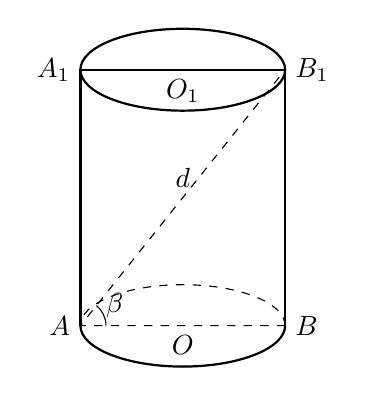
\begin{tikzpicture}[scale=1.3]
\draw[dashed](0,0) ellipse [x radius=1cm, y radius=.4cm];
\draw[thick](0,2.5) ellipse [x radius=1cm, y radius=.4cm];
\draw[thick](-1,0)node[left]{$A$}--(-1,2.5)node[left]{$A_1$}--(1,2.5)node[right]{$B_1$}--(1,0)node[right]{$B$};
\draw[thick](1,0) arc [x radius=1cm, y radius=.4cm, start angle =0, end angle =-180];
\draw[dashed](1,0)--(-1,0)--node[above]{$d$}(1,2.5);
\node at (0,0)[below]{$O$}; \node at (0,2.5)[below]{$O_1$};
\draw(-.75,0) arc (0:51.34:.25)node[right]{$\beta$};
\tkzDrawPoint(0,0)\tkzDrawPoint(0,2.5)
\end{tikzpicture}
    \caption{}
\end{figure}


\begin{solution}
    如图2.47, 已知圆柱$AA_1$, $B_1A$
    是其轴截面的一条对角线.因为$B_1A$与圆
    柱底面所成的角为$\beta$, 而$B_1B$垂直底面,所
    以$\angle B_1BA=90^{\circ}$, $\angle B_1AB=\beta$, 由$AB_1=d$,
    
$\therefore\quad B_1B=d\sin\beta$\quad 底面半径$OB=\frac{1}{2}d\cos\beta$

$\therefore\quad$ 底面圆周长$C=2\pi\cdot \frac{d}{2}\cos\beta=\pi d\cos\beta$

\[\begin{split}
    S_{\text{圆柱侧}}=C\cdot B_1B&=\pi d\cos\beta\cdot d\sin\beta\\ 
&=\pi d^2\cos\beta\cdot \sin\beta=\frac{1}{2}\pi d^2\sin2\beta
\end{split}\]
又$\because\quad |\sin2\beta|\le 1$

$\therefore\quad $当$\sin2\beta=1$时,即$2\beta=\frac{\pi}{2},\quad \beta=\frac{\pi}{4}$
时,$ S_{\text{圆柱侧}}=\frac{1}{2}\pi d^2$最大.

答:圆柱的侧面积为$\frac{1}{2}\pi d^2\sin2\beta$;当$\beta=\frac{\pi}{4}$时,圆柱的侧面积最大,这个最大值
是$\frac{1}{2}\pi d^2$.
\end{solution}

\begin{ex}
\begin{enumerate}
    \item 一长方体的三度之比为1:2:3, 其全面积为88, 求三度之
    长.
    \item 一直平行六面体的侧棱长为9cm, 底面相邻两边的长分
    别是7cm和11cm, 夹角是$45^{\circ}$, 求此平行六面体的全面
    积.
    \item 试证:两个等高圆柱侧面积的比等于它们半径的比.
    \item \begin{enumerate}
    \item 通过等边圆柱两底中心的轴截面面积为9, 求它
    的侧面积.
    \item 等边圆柱的全面积为$24\pi$, 
    求它底面的半径.
    \end{enumerate}

    \item 按照如图所示的两个视图,
    说明它们所表示的物体的形
    状,并画出它们的直观图,
    分别求出它们的全面积(视
    图(1)、(2)中所标尺寸单位为mm).
\end{enumerate} 
\end{ex}

\begin{figure}[htp]
    \centering
\begin{tikzpicture}[>=latex]
\begin{scope}
\draw(0,0) rectangle (2,1.5);
\draw(0,2)--(2,2)--(0,3.5)--(0,2);
\draw(2.5,2) rectangle (4,3.5);
\node at (2.5,-1){(1)};

\draw(0,0)--(0,-.5);   \draw(2,0)--(2,-.5);
\draw[<->](0,-.3)--node[fill=white]{$40$}(2,-.3);

\draw(2,0)--(2.5,0);  \draw(2,1.5)--(2.5,1.5);
\draw[<->](2.3,0)--node[fill=white, rotate=90]{$30$}(2.3,1.5);

\draw(4,2)--(4.5,2);  \draw(4,3.5)--(4.5,3.5);
\draw[<->](4.3,2)--node[fill=white, rotate=90]{$30$}(4.3,3.5);
\end{scope}
\begin{scope}[xshift=9cm, yshift=1cm]
\draw(1,0)--(60:1)--(120:1)--(-1,0)--(-120:1)--(-60:1)--(1,0);
\draw[dashdotted](-2,0)--(2,0);
\draw[dashdotted](0,-1.5)--(0,4);
\draw(-1,1.5) rectangle (1,3.5);
\draw(-.5,1.5)--(-.5,3.5);\draw(.5,1.5)--(.5,3.5);

\draw(1,1.5)--(1.5,1.5);  \draw(1,3.5)--(1.5,3.5);
\draw[<->](1.3,1.5)--node[fill=white, rotate=90]{$100$}(1.3,3.5);
\draw[|<->|](-.5,-1.25)--node[fill=white]{50}(.5,-1.25);
\draw[|<->|](1+.3,-.15)--node[fill=white, rotate=60]{50}+(-120:1);
\node at (0,-2){(2)};
\end{scope}
\end{tikzpicture}
    \caption*{第5题}
\end{figure}

\subsection{棱锥和圆锥的侧面积和全面积}

棱锥的侧面积等
于它的各个侧面面积之和,棱锥的全面积等于它的侧面积和
底面积的和.

设正棱锥的底面边长为$a$, 而它的斜高为$\ell$, 那么它的一
个侧面的面积就等于$\frac{1}{2}a\ell$,而所有侧面面积的和:
\[S_{\text{正棱锥侧}}=\frac{1}{2}na\ell\]

设p是底面周长,则$p=na$, 
所以,
\[S_{\text{正棱锥侧}}=\frac{1}{2}p\ell\]
由此可得下面定理.

\begin{blk}
    {定理} 如果正棱锥的底面周长是$p$, 斜高是$\ell$, 那么它的
    侧面积计算公式是:
    \[S_{\text{正棱锥侧}}=\frac{1}{2}p\ell\]
\end{blk}

\begin{blk}
    {推论} 正棱锥的全面积等于它的侧面积与底面积之和.
\end{blk}

如果把圆锥侧面沿着它的一条母线展开在平面上,如图
2.48所示,圆锥侧面的展开图是一个扇形,这个扇形的弧长
等于圆锥的底面周长$C$, 如果底面半径为$R$, 则$C=2\pi R$, 扇
形的半径等于圆锥的母线$\ell$, 而这个扇形的面积就是圆锥的
侧面积.由此可得下面定理.

\begin{figure}[htp]
    \centering
\begin{tikzpicture}[>=latex]
\begin{scope}
\draw[dashed] (0,0) ellipse [x radius=1, y radius=.4];
\draw[thick](-1,0)--(0,3)--node[right]{$\ell$}(1,0);
\draw[dashed](0,3)--(0,0)--node[above]{$R$}(1,0);
\draw(0,2.5) arc (90:90-18.43:.5) node[below]{$\tfrac{\alpha}{2}$};
\draw[thick](1,0) arc  [x radius=1, y radius=.4, start angle =0, end angle =-180];
\end{scope}
\begin{scope}[xshift=4cm, yshift=3cm]
\draw(0,0)--(3.16,0) arc (0:-114:3.16)--(0,0);
\draw(0,0)--(0,.5); \draw(3.16,0)--(3.16,.5);
\draw[<->](0,.3)--node[fill=white]{$\ell$}(3.16,.3);
\draw (.25,0)arc (0:-114:.25)node[below right]{$\theta$};
\draw(3.16,0)--(3.8,0);
\draw(-114:3.16)--(-114:3.8);
\draw[<->](3.6,0) arc (0:-114:3.6);
\node at (-100:3.6)[fill=white, right]{$C=2\pi R$};
\draw(-30:3.16+1) circle (1);
\draw[->](-30:3.16+1)--node[above]{$R$}+(-15:1);
\end{scope}
\end{tikzpicture}
    \caption{}
\end{figure}

\begin{blk}
    {定理}如果圆锥底面半径是$R$, 周长是$C$, 侧面母线长
是$\ell$, 那么它的侧面积计划公式是
\[S_{\text{圆锥侧}}=\frac{1}{2}C\ell =\pi R\ell\]
\end{blk}

\begin{blk}
    {推论1} 圆锥的全面积等于它的侧面积和底面积之和.即
    \[S_{\text{圆锥全}}=\pi R\ell +\pi R^2=\pi R(\ell+R)\]
\end{blk}

\begin{blk}
    {推论2} 如果设圆锥的展开面扇形的中心角为$\theta$, 圆锥
    的轴截面的顶角为$\alpha$, 那么
    \[\theta=\frac{2\pi R}{\ell}=2\pi \frac{R}{\ell}(\text{弧度})\]
或
\[\theta=360^{\circ}\frac{R}{\ell}=360^{\circ}\sin\frac{\alpha}{2}\]
\end{blk}

\begin{example}
    已知三棱锥$V$-$ABC$中,直角$\triangle ABC$的两条直角
边$AB=6$cm, $BC=8$cm, 高$VO=12$cm, 并且$O$点是$\triangle ABC$的
内心,求棱锥的全面积.
\end{example}


\begin{solution}
    如图2.49, 过$\triangle ABC$的
内心$O$作$OD\bot AB$于$D$, $OE\bot BC$
于$E$, $OF\bot AC$于$F$, 连结$VD$、
$VE$、$VF$.

$\because \quad VO\bot$底面$ABC$,

$\therefore\quad OD$是$VD$在底面$ABC$上
的射影,由三垂线定理,有$VD\bot AB$.

同理,$VE\bot BC$, $VF\bot AC$

$\because\quad OD=OE=OF=\frac{S_{\triangle ABC}}{\tfrac{1}{2}(AB+BC+AC)}=\frac{24}{12}=2$

$\therefore\quad VD=VE=VF=2\sqrt{37}$

$\therefore\quad S_{\triangle VAB}=\frac{1}{2}AB\cdot VD=\frac{1}{2}\cdot 6\cdot 2\sqrt{37}=6\sqrt{37}$
\[\begin{split}
    S_{\triangle VBC}&=\frac{1}{2}BC\cdot VE=\frac{1}{2}\cdot 8\cdot 2\sqrt{37}=8\sqrt{37}\\
S_{\triangle VAC}&=\frac{1}{2}AC\cdot VF=\frac{1}{2}\cdot 10\cdot 2\sqrt{37}=10\sqrt{37}
\end{split}\]
因此:
\[\begin{split}
    S_{\text{三棱锥全}}&=S_{\triangle ABC}+S_{\triangle VAB}+S_{\triangle VBC}+S_{\triangle VAC}\\
&=24+6\sqrt{37}+8\sqrt{37}+10\sqrt{37}\\
&=24+24\sqrt{37}\approx 169.9({\rm cm^2})
\end{split}\]

答:这个三棱锥的全面积约为$169.9{\rm cm^2}$.
\end{solution}

\begin{figure}[htp]\centering
    \begin{minipage}[t]{0.48\textwidth}
    \centering
\begin{tikzpicture}[>=latex, scale=1]
\tkzDefPoints{0/0/A, 3/0/B, 4.5/1.8/C, 2.5/4/V, 2.5/.5/O}
\tkzDrawPolygon(A,B,C,V)
\tkzDrawSegments[dashed](A,C V,O)

\tkzDefPointWith[linear, K=.7](A,B)  \tkzGetPoint{D}
\tkzDefPointWith[linear, K=.55](C,B)  \tkzGetPoint{E}
\tkzDefPointWith[linear, K=.38](A,C)  \tkzGetPoint{F}

\tkzDrawSegments[dashed](D,O O,E O,F V,F)
\tkzDrawSegments (V,D V,E V,B)
\tkzLabelPoints[below](A,B,D,O)
\tkzLabelPoints[above](V,F)
\tkzLabelPoints[right](C,E)
    \end{tikzpicture}
    \caption{}
    \end{minipage}
    \begin{minipage}[t]{0.48\textwidth}
    \centering
    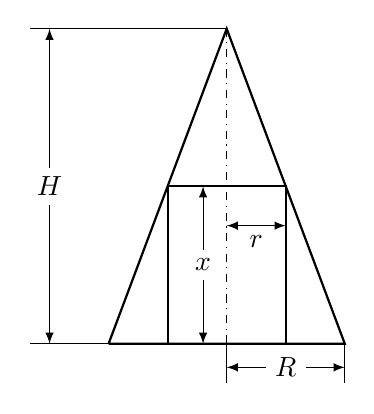
\begin{tikzpicture}[>=latex, scale=1]
\draw[thick](0,0)--(3,0)--(1.5,4)--(0,0);
\draw[thick](.75,2) rectangle (3-.75,0);
\draw[dashdotted](1.5,0)--(1.5,4);
\draw(-1,0)--(0,0);  \draw(-1,4)--(1.5,4);
\draw[<->](-.75,0)--node[fill=white]{$H$}(-.75,4);
\draw(1.5,0)--(1.5,-.5); \draw(3,0)--(3,-.5); 
\draw[<->](1.5,-.3)--node[fill=white]{$R$}(3,-.3);
\draw[<->](1.2,0)--node[fill=white]{$x$}(1.2,2);
\draw[<->](1.5,1.5)--node[below]{$r$}(3-.75,1.5);
    \end{tikzpicture}
    \caption{}
    \end{minipage}
    \end{figure}

\begin{example}
    已知一个圆锥的底面半径为$R$, 高为$H$, 在其中有
一个高为$x$内接圆柱.
\begin{enumerate}
    \item 求圆柱的侧面积.
    \item $x$为何值时,圆柱的侧面积最大?
\end{enumerate}
\end{example}

\begin{solution}
\begin{enumerate}
    \item 画圆锥及其内接圆柱的轴截面图(图2.50)
    
    设内接圆柱的底面半径为$r$, 圆锥的底面半径为$R$. 那么内接
    圆柱的侧面积
 \[   S_{\text{圆柱侧}}=2\pi rx\]
又$\because\quad \frac{r}{R}=\frac{H-x}{H}$

$\therefore\quad r=R-\frac{R}{H}x$

$\therefore\quad S_{\text{圆柱侧}} =2\pi Rx-\frac{2\pi R}{H}x^2$

\item 因为$S_{\text{圆柱侧}}$的表示式中,$x^2$的系数小于零,所以
    这个二次函数有最大值,当这个二次函数达到最大值时,圆
    柱的侧面积最大.这时圆柱的高是
\[x=-\frac{2\pi R}{-2\cdot \frac{2\pi R}{H}}=\frac{H}{2}\]

答:当圆柱的高是已知高一半时,它的侧面积最大.
\end{enumerate}    
\end{solution}

\begin{example}
    若圆锥的侧面积等于和它等高、等底的圆柱的侧
面积时,求圆锥轴截面顶角的度数.
\end{example}

\begin{figure}[htp]
    \centering
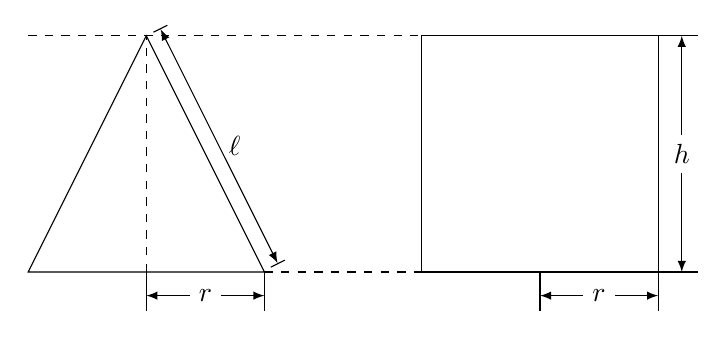
\begin{tikzpicture}[>=latex]
\draw(0,0)--(-1.5,3)--(-3,0)--(0,0);
\draw[dashed](-1.5,0)--(-1.5,3);
\draw[dashed](-3,3)--(2,3);
\draw[dashed](0,0)--(2,0);
\draw (2,0) rectangle (5,3);

\draw(-1.5,0)--(-1.5,-.5);\draw(0,0)--(0,-.5);
\draw[<->](-1.5,-.3)--node[fill=white]{$r$}(0,-.3);
\draw[|<->|](30:.2)--node[right]{$\ell$}+(180-63.43:3.35);
\draw(3.5,0)--(3.5,-.5);\draw(5,0)--(5,-.5);
\draw[<->](3.5,-.3)--node[fill=white]{$r$}(5,-.3);

\draw(5,0)--(5+.5,0);\draw(5,3)--(5+.5,3);
\draw[<->](5.3,0)--node[fill=white]{$h$}(5.3,3);
\end{tikzpicture}
    \caption{}
\end{figure}

\begin{solution}
    如图2.51, 设圆锥、圆柱的高为$h$, 底面半径为$r$, 则
\[\begin{split}
    S_{\text{圆柱侧}}&=2\pi rh\\
S_{\text{圆锥侧}} &=\pi r\ell=\pi r\sqrt{h^2+r^2}
\end{split}\]
根据已知条件,
\[\begin{split}
    2\pi rh&=\pi r\sqrt{h^2+r^2}\\
\frac{h}{\sqrt{h^2+r^2}}&=\frac{1}{2}
\end{split}\]
即:$\cos\frac{\alpha}{2}=\frac{1}{2}$,$0^{\circ}<\alpha<180^{\circ}$

$\therefore\quad \frac{\alpha}{2}=60^{\circ},\qquad \alpha=120^{\circ}$

答:轴截面顶角等于$120^{\circ}$.
\end{solution}

\begin{ex}
\begin{enumerate}
    \item 正四棱锥的底面边长是$a$, 高是$2a$, 计算它的全面积.
    \item 一个正三棱锥的侧面都是直角三角形,底面边长是$a$, 
    求它的全面积.
    \item 圆锥母线和底面夹角是$30^{\circ}$, 求它的侧面展开图的圆心
    角.
    \item 将半径为$r$的薄圆铁板沿它的三条半径截成全等的三个
    扇形,作成三个圆锥筒,求圆锥筒的高(不计接头).
    \item 
    将一个半圆卷成圆锥的侧面,求这圆锥母线和高的夹
    角.
    \item 求底面边长为$2a$, 高为$2a$的正四棱锥的内切圆锥的侧面
    积.
    \item 已知正三棱锥$V$-$ABC$, 底
    面每边长为$a$, 侧棱和底面
    所成的角为$45^{\circ}$, 求它的全
    面积.
\end{enumerate}
\end{ex}

\begin{figure}[htp]
    \centering
\includegraphics[scale=.6]{fig/6ti.png}
    \caption*{第6题}
\end{figure}

\subsection{棱台和圆台的侧面积和全面积 }
棱台的每个侧面都是梯形,所有这些侧面面积之和就
是棱台的侧面积,棱台的全面积
等于它的侧面积和两个底面积的
和.

如果棱台是正棱台,那么它的每个侧面都是全等的等腰
梯形,设它的上、下底边长分别是$a'$和$a$, 边数是$n$, 斜高是
$h'$, 那么它的侧面积是
\[n\cdot \frac{1}{2}(a'+a)h'=\frac{1}{2}(na+na')h'\]

由于$na'$、$na$分别是上、下底的周长,设$na'=p'$, 
$na=p$, 我们就得到下面定理.

\begin{blk}
   {定理} 如果正棱台的上、下底的周长分别为$p'$和$p$, 斜
高是$h'$, 那么它的侧面积的计算公式是 
\[S_{\text{正棱台侧}}=\frac{1}{2}(p+p')h'\]
\end{blk}

显然,在正棱台的侧面积计算公式中,如果$p'=p$, 就
得到正棱柱的计算公式:
\[S_{\text{正棱柱侧}}=ph'\]
这里$h'$为高.

如果$p'=0$, 就得到正棱锥的侧面积计算公式:
\[S_{\text{正棱锥侧}}=\frac{1}{2}ph'\]

\begin{blk}
   {推论} 正棱台的全面积等于它的侧面积和两个底面积的
和. 
\end{blk}

圆台的侧面展开图以看成是两个圆锥侧面展开图的
差,通常把这种图形叫做扇环.如图2.52所示.
\begin{figure}[htp]
    \centering
\begin{tikzpicture}[>=latex]
    \tkzDefPoints{0/0/V}
\tkzDefPoint(40:2){A'_1}
\tkzDefPoint(40:3.5){A'}
\tkzDefPoint(-60:2){A_1}
\tkzDefPoint(-60:3.5){A}
\tkzDefPoint(-120:2){B}
\tkzDefPoint(-120:3.5){B'}
\draw(0,-1.732) ellipse [x radius=1, y radius=.3];
\draw (0,-1.732)node[left]{$O_1$}--node[below]{$R_1$}(A_1)node[above]{$A_1$};
\tkzDrawSegments[dashed](V,A'_1 V,A_1 V,B)
\tkzDrawSegments(A',A'_1 A,A_1 B,B')
\draw(A) arc [x radius=1.75, y radius=.4, start angle =0, end angle =-180];
\draw[dashed](A) arc [x radius=1.75, y radius=.4, start angle =0, end angle =180];
\draw[dashed] (0,-1.75*1.732)node[left]{$O$}--node[above]{$R$}(A)node[below right]{$A$};
\draw(A_1) arc (-60:40:2);
\draw(A) arc (-60:40:3.5);
\tkzLabelPoints[above](A'_1,A',V)
\draw[<->](-52:2)--node[fill=white]{$\ell$}(-52:3.5);
\tkzMarkAngle[mark=none, size=.3](A,V,A')
\tkzLabelAngle[pos=.7](A,V,A'){$\theta$}
\node at (-20:2.25)[rotate=70]{$C_1=2\pi R_1$};
\node at (-20:3.75)[rotate=70]{$C=2\pi R$};
\end{tikzpicture}
    \caption{}
\end{figure}


圆台的侧面展开图是一个大扇形去掉一个小扇形.大扇
形的弧长是圆台下底的圆周长$C_1$, 小扇形弧长是圆台上底圆
周长$C$, 设圆台的母线$AA_1=\ell$, 上、下底半径分别是$R_1$和
$R$, 于是
\[S_{\text{圆台侧}}=S_{\text{扇形}VAA'}-S_{\text{扇形}VA_1A_1'}=\frac{1}{2}CVA-\frac{1}{2}C_1VA_1\]

于是问题归结为求$VA$和$VA_1$, 因为$C_1$和$C$所张的圆心角是同一个角$\theta$, 则
\[\frac{C_1}{VA_1}=\frac{C}{VA}\]
即
\[\frac{VA-\ell}{VA}=\frac{C_1}{C}\]
因此:
\begin{equation}
VA=\frac{C\ell}{C-C_1},\qquad VA-\ell=\frac{C_1\ell}{C-C_1}    
\end{equation}
所以:
\begin{equation}
    \begin{split}
S_{\text{圆台侧}}=\frac{1}{2}\cdot\frac{C^2\ell}{C-C_1}-\frac{1}{2}\cdot \frac{C^2_1\ell}{C-C_1}&=\frac{1}{2}\cdot\frac{(C^2-C^2_1)\ell}{C-C_1}\\
&=\frac{1}{2}(C_1+C_2)\ell        
    \end{split}
\end{equation}

$\because\quad C=2\pi R,\quad  C_1=2\pi R_1$,代入(2.10)

$\therefore\quad S_{\text{圆台侧}}=\pi(R+R_1)\ell$

由此,我们得到下面定理

\begin{blk}
    {定理} 如果圆台的上、下底半径分别是$R_1$和$R$, 周长分别是$C_1$和$C$, 那么圆台的侧面积计算公式是
\[S_{\text{圆台侧}}=\frac{1}{2}(C_1+C)\ell=\pi(R_1+R)\ell \]
\end{blk}

\begin{blk}{推论}
\begin{enumerate}
    \item 圆台的全面积等于它的侧面积与上、下两个底面积的和
    \item $\theta=2\pi\frac{R-R_1}{\ell}(\text{弧度})\quad \text{或}\quad \theta=360^{\circ}\frac{R-R_1}{\ell}$
\end{enumerate}
显然,在圆台的侧面积公式中,如果$C_1=C$, 就得到圆柱侧面积公式:$S_{\text{圆柱侧}}=C\ell$; 如果$C_1=0$, 就得到圆锥的侧面积公式:$S_{\text{圆锥侧}}=\frac{1}{2}C\ell$.
\end{blk}



\begin{example}
粉碎机的下料斗是正四棱台(图2.53). 它的两底边长分别是80mm和440mm, 高是200mm, 计算制造这样一个下料斗所需铁板面积.(保留两位有效数字)
\end{example}

\begin{solution}
由于:
\[\begin{split}
    \text{上底周长}p'&=4\x80=320{\rm (mm)}\\
    \text{下底周长}p&=4\x440=1760{\rm (mm)}\\
    \text{斜高}h'&=\sqrt{200^2+ \left(\frac{440-80}{2}\right)^2}\approx 269 {\rm (mm)}
\end{split}\]
所以:
\[S_{\text{正棱台侧}}=\frac{1}{2}(p+p')h'\approx \frac{1}{2}(320+1760)\x 269\approx 2.8\x 10^5 ({\rm mm^2})\]
答:制造这样一个下料斗需要的铁板约为$2.8\x 10^5 {\rm mm^2}$.
\end{solution}

\begin{figure}[htp]
    \centering
    \begin{minipage}[t]{0.48\textwidth}
    \centering
    \begin{tikzpicture}[>=latex, scale=1]
\tkzDefPoints{0/0/A, 2/0/B, 3/1/C}
\tkzDefPointsBy[translation = from B to C](A){D}
\tkzDefPoints{-1.5/3/A', 3/3/B', 4.5/4.5/C'}
\tkzDefPointsBy[translation = from B' to C'](A'){D'}
\tkzDrawPolygon(A',B',C',D')
\tkzDrawSegments(A,A' B,B' C,C' A,B B,C)
\tkzDrawSegments[dashed](D,D' C,D D,A)
\tkzInterLL(A,C)(B,D) \tkzGetPoint{E}
\tkzInterLL(A',C')(B',D') \tkzGetPoint{E'}
\tkzDefMidPoint(B,C) \tkzGetPoint{F}
\tkzDefMidPoint(B',C') \tkzGetPoint{F'}
\tkzDrawSegments[dashed](E,E' E,F E',F')
\tkzDrawSegments(F,F')
\tkzLabelSegment[right](F,F'){$h'$}
\tkzLabelSegment[right](E,E'){$h$}
\end{tikzpicture}
    \caption{}
    \end{minipage}
    \begin{minipage}[t]{0.48\textwidth}
    \centering
    \begin{tikzpicture}[>=latex, scale=1]
\begin{scope}
\tkzDefPoints{-1.5/0/A, 1.5/0/B, 0/2/C}
\tkzDefPointWith[linear, K=0.333](C,A) \tkzGetPoint{A'}
\tkzDefPointWith[linear, K=0.333](C,B) \tkzGetPoint{B'}
\tkzDrawPolygon(A,B,B',A')
\tkzDrawSegments[dashed](C,A' C,B')
\tkzLabelSegment[right](C,B'){$x$}
\tkzLabelSegment[right](B,B'){$\ell$}
\node at (.75,0)[above]{3};
\node at (.5,4/3)[below]{1};
\draw(0,0)--(0,4/3);
\draw[dashed](0,4/3)--(0,2);
\node at (2,1)[right]{(1)};
\end{scope}
\begin{scope}[yshift=-2cm]
\draw(0,0) circle (.5);
\draw(0,0) circle (1.5);
\draw[dashed](0,-.5)--node[left]{$x$}(0,0)--(45:.5);
\draw(0,-.5)--(0,-1.5);
\draw(45:.5)--node[above]{$\ell$}(45:1.5);
\node at (2,0)[right]{(2)};

\end{scope}
    \end{tikzpicture}
    \caption{}
    \end{minipage}
  \end{figure}
  


\begin{example}
    一个圆台的两个底的半径是1和3, 侧面展开图是圆环的一部分,已知全圆环的面积和这个圆台的全面积相等,求这圆台母线长,侧面积和全面积.
\end{example}


\begin{solution}
设图2.54(1)是圆台的轴截面,设$x$是截去的小圆锥的母线长,$\ell$为圆台的母线,根据已知条件,有
\[\frac{x+\ell}{x}=\frac{3}{1}\]

$\therefore\quad x=\frac{1}{2}\ell$

又$\because\quad \pi\cdot 1^2+\pi\cdot 3^2+\pi\ell(1+3)=\pi\left[\left(\frac{3\ell}{2}\right)^2-\left(\frac{1}{2}\ell\right)^2\right]$

即:$\ell^2-2\ell-5=0$

$\therefore\quad \ell=\frac{2\pm\sqrt{4+20}}{2}=1+\sqrt{6}$ (由于$\ell>0$, 故舍去负根)

因此:
\[\begin{split}
S_{\text{圆台侧}}&=\pi \ell(R+R_1)=\pi  (1+\sqrt{6}) (1+3)=4\pi  (1+\sqrt{6})\\
S_{\text{圆台全}} &=4\pi (1+\sqrt{6})+\pi \cdot 1^2+\pi \cdot 3^2
=14\pi +4\pi \sqrt{6}=2\pi  (7+2\sqrt{6})
\end{split}\]

答:圆台的母线长为$(1+\sqrt{6})$, 侧面积为$4\pi(1+\sqrt{6})$, 全面积为$2\pi (7+2\sqrt{6})$.
\end{solution}

\begin{ex}
\begin{enumerate}
    \item 正四棱台两底面边长分别为8m和2m, 高是4m, 求它的
    全面积.
    \item 正三棱台的两底的边长分别为6dm和12dm, 高为1dm,
    求它的侧面积.
    \item 一个正三棱台的上、下底面的边长分别是$a,b$, 侧面与
    底面成$60^{\circ}$的二面角,求它的全面积.
    \item 正四棱台的上、下两底面边长分别为$a,b$, 其侧面面积
    等于两底面积之和,求此棱台的高.
    \item 一个圆台的高为3cm, 一个底面半径是另一个底面半径
    的2倍,母线和下底的夹角为$45^{\circ}$, 求它的侧面积.
    \item 一个圆台的全面积等于$572\pi{\rm cm^2}$, 两底半径分别是6cm和14cm, 求这圆台的高.
\end{enumerate}
\end{ex}

\subsection{球面积和它的部分面积}

前面我们求圆柱、圆锥,圆台的侧面积公式都是利用它们的展开图求出的,由于球面不能展成平面图形,所以球的表面积计算公式无法用展开图求出,我们得另想计算方法.古希腊的几何学家欧都克斯为我们提供了一个在数学上非常有应用价值的逼近法来解决这个问题.

\begin{blk}
 {逼近原理} 设$\alpha$、$\alpha'$是两个实数,假如它们同时被一个递增数列$\{a_n\}$和一个递减数列$\{b_n\}$所左右夹逼,而且$(b_n -a_n)$在$n$增大时,可以任意小,即
\[a_1\le a_2\le \cdots\le a_n<\cdots<\alpha,\qquad \alpha'<\cdots\le b_n\le \cdots\le b_2\le b_1\] 
 且当$n$无限增大时,$(b_n-a_n)\to 0$, 则$\alpha$必须等于$\alpha'$.   
\end{blk}

换句话说,上述左右夹逼数列唯一地确定了界于其间的那个实数$\alpha$.

为了求得球面积的部分面积计算公式,我们还需要下面的预备知识.

\begin{blk}
  {定义} 如果平面内的一条折线,它所有的边都相等,并且相邻两边的夹角也都相等,那么这个平面折线叫做正折线.
\end{blk}

\begin{blk}
   {推论} 正折线都有一个中心,它是到正折线各顶点距离都相等,并且到各边距离相等的一个点.   
\end{blk}


\begin{blk}
    {引理1} 一条线段绕着和它在同一平面内并且至多有和它的一个端点相交的轴旋转所生成的旋转面的面积(即圆柱、圆锥、圆台的侧面积)等于一个圆柱的侧面积,这个圆柱的高等于这线段在轴上的射影,而它的底面半径等于以母线为底边,两顶点在轴上的等腰三角形的高.
\end{blk}

已知:如图2.55所示,线段$AB$与轴$XY$在同一平面内,$MR$垂直平分线段$AB$于$M$, 且与$XY$轴交于$R$, $CD$是$AB$在$XY$上的射影,$MO\bot XY$于$O$, $S_{AB}$是线段$AB$旋转面的面积

求证:$S_{AB}=2\pi MR\cdot CD$

\begin{figure}[htp]
    \centering
\begin{tikzpicture}[scale=.7]
\draw[dashdotted](0,0)node[left]{$X$}--(15,0)node[right]{$Y$};
\foreach \x in {4,9,14}
{
    \draw(\x,0) ellipse [x radius=.5, y radius=1.5];
    \draw[dashed](\x,0)node[below]{$D$}--(\x, 1.5)node[above]{$B$};
}

\draw(1.5,1.5) arc [start angle=90, end angle =270, x radius=.5, y radius=1.5];
\draw[dashed](1.5,1.5)node[above]{$A$}--(1.5,0)node[below]{$C$};
\draw[dashed](2.75,1.5)node[above]{$M$}--(2.75,0)node[below]{$R$};
\draw(1.5,-1.5)--(4,-1.5); \draw(1.5,1.5)--(4,1.5);

\draw(9,-1.5)--(6.5,0)node[below]{$(C)$};
\draw(6.5,0)node[above]{$A$}--(9,1.5);
\draw[dashed](7.75,0.75)node[above]{$M$}--(7.75,0)node[below]{$O$};
\draw[dashed](7.75,0.75)--(8.2,0)node[below]{$R$};

\draw(11.5,.8) arc [start angle=90, end angle =270, x radius=.3, y radius=.8];
\draw[dashed](11.5,.8)node[above]{$A$}--(11.5,0)node[below]{$C$};
\draw[dashed](12.75,1.15)node[above]{$M$}--(12.75,0)node[below]{$O$};
\draw(11.5,-.8)--(14,-1.5); \draw(11.5,.8)--(14,1.5);
\draw[dashed](11.5,.8)--(14,.8)node[right]{$E$};
\draw[dashed](12.75,1.15)--(13.2,0)node[below]{$R$};

\end{tikzpicture}
    \caption{}
\end{figure}

\begin{proof}
\begin{enumerate}
    \item 若线段$AB\parallel XY$, 则$CD=AB$, $MO$与$MR$重合,
    
$\because\quad MR=BD,\quad  AB=CD$

$\therefore\quad S_{\text{圆柱侧}}=2\pi BD\cdot AB=2\pi MR\cdot CD$
    \item 若线段$AB$的端点$A$在$XY$上,

$\because\quad   \angle BAD=\angle RMO,\quad \angle MOR=\angle BDA=90^{\circ}$

$\therefore\quad \triangle OMR\backsim \triangle DAB$

$\therefore\quad \frac{MR}{AB}=\frac{MO}{AD}=\frac{BD}{2AD},\quad 2MR\cdot AD=AB\cdot BD$

$\therefore\quad S_{\text{圆锥侧}}=\pi BD\cdot AB=2\pi MR\cdot CD$($A$点与$C$点重合)
    \item 若线段$AB$不平行$XY$又不与$XY$相交,作$AE\parallel XY$设与$BD$交于$E$.

$\because\quad \angle BAE=\angle RMO,\quad \angle MOR=\angle AEB=90^{\circ}$    

$\therefore\quad \triangle AEB\backsim \triangle MOR$

$\therefore\quad AB\cdot MO=AE\cdot MR$

$\because\quad AE=CD$

$\therefore\quad AB\cdot MO=CD\cdot MR$

$\therefore\quad S_{\text{圆台侧}}=2\pi MR\cdot CD$
\end{enumerate}
\end{proof}

    本引理的结论可以看成是求圆柱、圆锥、圆台侧面积的一般公式.

\begin{blk}
    {引理2}一条正折线,绕着轴(这个轴是一条在折线所在平面内的直线,它过折线的中心并且不穿过折线)旋转所得的旋转体的侧面积等于一个圆柱的侧面积,这个圆柱的底面半径等于折线的边心距,而高等于折线在旋转轴上的射影.
\end{blk}

已知:一条正折线$ABCDE$ (图2.56) 绕着过折线中心$O$的轴$XY$旋转,所得的旋转面面积如图2.57所示,设它
为$S$; 
令$h=OM=ON=OP=OQ$表示折线的边心距;用$ab$, $bc$, $cd$, $de$分别表示线段$AB$、$BC$、$\ldots DE$在轴$XY$上的射影.

求证:$S=2\pi h(ae)$

\begin{figure}[htp]
    \centering
    \begin{minipage}[t]{0.48\textwidth}
    \centering
    \begin{tikzpicture}[>=latex, scale=1]
\draw(0,-2)node[below]{$Y$}--(0,2.5)node[above]{$X$};
\tkzDefPoints{-.5/-1.5/E, -1.5/-.6/D, -1.5/.6/C, -1/1.3/B, 0/1.7/A, 0/0/o}
\tkzDefMidPoint(A,B) \tkzGetPoint{M}
\tkzDefMidPoint(C,B) \tkzGetPoint{N}
\tkzDefMidPoint(C,D) \tkzGetPoint{P}
\tkzDefMidPoint(D,E) \tkzGetPoint{Q}
\tkzDrawSegments(A,B B,C C,D D,E M,o N,o P,o Q,o)
\tkzDefPointBy[projection = onto A--o](B) \tkzGetPoint{b}
\tkzDefPointBy[projection = onto A--o](C) \tkzGetPoint{c}
\tkzDefPointBy[projection = onto A--o](D) \tkzGetPoint{d}
\tkzDefPointBy[projection = onto A--o](E) \tkzGetPoint{e}
\tkzDrawSegments[dashed](B,b C,c D,d E,e)
\tkzLabelPoints[right](b,c,d,e,o)
\node at (A)[right]{$a$};
\tkzAutoLabelPoints[center=o](B,C,D,E,M,N,P,Q)
\tkzLabelPoints[above left](A)
    \end{tikzpicture}
    \caption{}
    \end{minipage}
    \begin{minipage}[t]{0.48\textwidth}
    \centering
    \begin{tikzpicture}[>=latex, scale=1]
\draw(0,-2)node[below]{$Y$}--(0,2.5)node[above]{$X$};
\tkzDefPoints{-.5/-1.5/E, -1.5/-.6/D, -1.5/.6/C, -1/1.3/B, 0/1.7/A, 0/0/o}
\tkzDrawSegments[thick](A,B B,C C,D D,E)
\tkzDefPointBy[reflection = over A--o](B) \tkzGetPoint{B'}
\tkzDefPointBy[reflection = over A--o](C) \tkzGetPoint{C'}
\tkzDefPointBy[reflection = over A--o](D) \tkzGetPoint{D'}
\tkzDefPointBy[reflection = over A--o](E) \tkzGetPoint{E'}
\tkzDrawSegments[thick](A,B' B',C' C',D' D',E')
\draw(B') arc [start angle=0, end angle =-180, x radius=1, y radius=.2];
\draw[dashed](B') arc [start angle=0, end angle =180, x radius=1, y radius=.15];

\draw(C') arc [start angle=0, end angle =-180, x radius=1.5, y radius=.3];
\draw[dashed](C') arc [start angle=0, end angle =180, x radius=1.5, y radius=.3];
\draw(D') arc [start angle=0, end angle =-180, x radius=1.5, y radius=.3];
\draw[dashed](D') arc [start angle=0, end angle =180, x radius=1.5, y radius=.3];
\draw(E') arc [start angle=0, end angle =-180, x radius=.5, y radius=.1];
\draw[dashed](E') arc [start angle=0, end angle =180, x radius=.5, y radius=.1];

  
    \end{tikzpicture}
    \caption{}
    \end{minipage}
  \end{figure}

  
\begin{proof}
    当正折线$ABCDE$旋转时,它的每一条边,便分
别画出一个圆锥、圆台或者圆柱的侧面,根据圆柱、圆锥、圆台的求侧面积的一般公式,正折线的边$AB$、$BC$、$CD$和$DE$旋转所得的旋转面的面积分别等于$2\pi h(ab)$、$2\pi h(bc)$、$2\pi h(cd)$和$2\pi h(de)$. 
因此:
\[S=2\pi h(ab+bc+cd+de)=2\pi h\cdot (ae)\]

我们可以把球面积看作半圆弧绕着它的直径旋转所得的面积,因为这半圆弧的内接正折线与外切正折线绕着直径旋转所得的面积是可求的(如前段所述),故我们先用半圆弧的内接正折线和外切正折线来夹逼这圆弧,当边数$n$增多
时,相应的内接正折线增大,愈来愈贴近半圆弧,而相应的外切正折线减小,也愈来愈贴近半圆弧,这就是说,内接正折线绕直径旋转所得面积数列与外切正折线绕直径旋转所得的面积数列,从左、右两方面愈来愈逼近球面积的值,从而我们就可以得到球面积公式.

为了以后讨论方便起见,我们先考虑半圆弧的一部分绕着该半圆弧的直径旋转所得的球的部分面积公式.

\begin{figure}[htp]
    \centering
\begin{tikzpicture}[>=latex, scale=1.1]
    \tkzDefPoints{0/0/O}
\foreach \xangle/\xtext in {40/E, 70/D, 100/C, 130/B, 160/A}
{
    \tkzDefPoint(\xangle:5){\xtext}
    \tkzDefPoint(\xangle:5*1.0353){\xtext'}
}
\tkzDrawPolygon(O,A,B,C,D,E)
\tkzDrawPolygon(O,A',B',C',D',E')
\tkzDrawArc[color=black](O,E)(A)
\tkzDrawSegments(O,B' O,C' O,D')
\tkzDefPoints{-5/0/K, 5/0/L}
\tkzDrawArc[color=black, dashed](O,L)(E)
\tkzDrawArc[color=black, dashed](O,A)(K)
\tkzDrawSegments(K,L)

\foreach \x/\y in {A/a, B/b, C/c, D/d, E/e}
{
    \tkzDefPointBy[projection= onto K--L](\x)
\tkzGetPoint{\y}    
\tkzDrawSegments[dashed](\x,\y)
}
\foreach \x/\y in {A'/a', B'/b', C'/c', D'/d', E'/e'}
{
    \tkzDefPointBy[projection= onto K--L](\x)
\tkzGetPoint{\y}    
\tkzDrawSegments[dashed](\x,\y)
}
\tkzLabelPoints[below](O)

\tkzLabelPoints[below left](a',b',c',d,e)
\tkzLabelPoints[below right](a,b,c,d',e')
\tkzAutoLabelPoints[center=O, pos=.93](A',B',C',D',E',K,L)
\tkzAutoLabelPoints[center=O, pos=.82](A,B,C,D,E)
\tkzDefPointBy[projection= onto A--B](O)
\tkzGetPoint{H}   
\tkzInterLC(O,H)(O,K)
\tkzGetPoints{T2}{H'}
\tkzLabelPoints[below](H)
\tkzLabelPoints[above](H')
\tkzDrawSegments(O,H')

\end{tikzpicture}   
    \caption{}
\end{figure}

如图2.58, 圆弧$AE$绕着和它不相交的直径旋转所得
部分球面,如图2.59所示.这部分平面可以用两个平行平面截球面得到.我们把夹在平行平面之间的球面部分叫做球带,两个平行截面间的距离叫做球带的高,记作$h$. 
\begin{figure}[htp]
    \centering
\begin{tikzpicture}
   \draw(2,0) arc (0:45:2); 
\draw(-2,0) arc (180:135:2);
\draw[dashed](0,0) ellipse [x radius=2, y radius=.4];
\draw(0,1.414) ellipse [x radius=1.414, y radius=.2];
\draw[dashed](0,0)--node[right]{$h$}(0,1.414);
\draw(2,0)node[right]{$E$}  arc [start angle =0, end angle =-180, x radius=2, y radius=.4];
\node at (1.414,1.414)[above]{$A$};
\end{tikzpicture}
    \caption{}
\end{figure}

作圆弧$AE$的内接正$n$边折线和外切正$n$边折线,$a$、$e$两点是圆弧$AE$的两端在直径$KL$上的正
射影.于是圆弧$AE$的内接正$n$边折线在直径$KL$上的射影是线段$ae$, 它是一个与边数$n$无关的定值,即$ae=h$.

设$h_n$为$\wideparen{AE}$的内接正$n$边折线的边心距.$\sigma_n$为内接正$n$边折线绕直径$KL$旋转所得的面积.半径$R$是$\wideparen{AE}$的外切正$n$边折线的边心距.线段$a'e'$是外切正$n$边折线在直径$KL$上的正射影.$S_n$ 为外切正$n$边折线绕直径$KL$旋转得到的面积.$S_{\text{球带}}$为圆弧$AE$绕直径$KL$旋转得到的球带面积.根据几何直观,我们得到
\begin{enumerate}
\item 当边数$n$增加时,$\sigma_n$递增,$S_n$递减.
\item $\sigma_n<S_{\text{球带}}<S_n$,且由引理2可知:
\[\sigma_n<2\pi h_n(ae)=2\pi h_n h,\qquad S_n =2\pi R (a'e')\]    
\end{enumerate}

显然,$h_n$随着$n$增大而增大,而且趋近于$R$, 换句话说,$(R-h_n)$可以任意小,即$(R-h_n)\to 0$. 

现在我们要进一步说明$a'e'$随$n$增大而减小,并且趋近于$ae=h$(球带高).

换言之,$a'e'-h$可以任意小,即$(a'e'-h)\to 0$. 因为,内接正折线与外切正折线对于圆心是位似形,其相似比是$\frac{R}{h_n}$,
由此得
\[\frac{a'e'}{ae}=\frac{R}{h_n}>1,\qquad a'e'=\frac{R}{h_n}\cdot h\]

当$n$增大时,$h_n$增大并且趋近于$R$, 于是$a'e'$减小,并且
愈来愈趋近$ae=h$. 这样我们就得到:
\[\sigma_n=2\pi h_n\cdot h<S_{\text{球带}}<2\pi R(a'e')=S\]
且当$n$增大时,$h_n\to R$, $a'e'\to h$.

最后,我们要说明,当$n$增大时,$S_n-\sigma_n$可以小到
任意小.

$\because\quad \frac{S_n}{\sigma_n}=\frac{R(a'e')}{h_n\cdot h}=\frac{R}{h_n}\cdot \frac{a'e'}{h}=\frac{R^2}{h^2_n},\quad \frac{S_n-\sigma_n}{S_n}=\frac{R^2-h^2_n}{R^2}$

$\therefore\quad S_n-\sigma_n=S_n\frac{(R+h_n) (R-h_n)}{R^2}$

又$\because\quad S_n<S_1,\quad R+h_n<2R$

$\therefore\quad S_n-\sigma_n<\frac{2S_1}{R}(R-h_n)$

故:当$n$增大时,$R-h_n$可任意小,从而,$S_n -\sigma_n$可以任意小.
这就是说$S_{\text{球带}}$应定义为夹逼数列$\{\sigma_n\}$和$\{S_n \}$所确定的那个数.

另一方面,由$h_n\to R$, $a'e'\to h$, 我们看出,恒有
\[\sigma_n=2\pi h_n\cdot h<2\pi R\cdot h<2\pi R (a'e') =S_n\]
根据逼近原理知
$$S_{\text{球带}}=2\pi R\cdot h$$
\end{proof}

于是我们得到下面的定理.

\begin{blk}
    {定理} 球带的面积等于截成它的球面上大圆周长与球带的高的积.即
\[S_{\text{球带}}=2\pi R\cdot h\]
\end{blk}

如果截球的两个平行平面都成为球的切面,那么$ae=$直径$=2R$. 那么球带就变成了整个球面,所以球面积$S_{\text{球}}=2\pi R\cdot 2R=4\pi R^2$.

由此,我们得到下面定理.

\begin{blk}
    {定理}球面面积等于它的大圆面积的四倍,即
\[S_{\text{球面}}=4\pi R^2\]
\end{blk}

如果截球的两个平行平面的一个成为切面,那么这时的球带所变成的球面部分叫做\textbf{球冠}.截平面得到的圆叫做球冠的\textbf{底面},垂直于截面的直径被截得的一段叫做球冠的\textbf{高},记作$h$. 如图2.60所示.

球冠也可以看作是一段圆弧绕经过它的一个端点的直径旋转得到的球面部分,这时,$ae=h$, 于是得到下面定理.


\begin{blk}
    {定理} 球冠的面积等于截它的球面上大圆周长与球冠的高的积,即
\[S_{\text{球冠}}=2\pi R\cdot h\]
\end{blk}

我们注意到球冠的面积公式与球带的面积公式相同.

\begin{figure}[htp]
    \centering
    \begin{minipage}[t]{0.48\textwidth}
    \centering
    \begin{tikzpicture}[>=latex, scale=.9]

\begin{scope}
    \draw(45:2)node[right]{$E$} arc (45:135:2);
    \draw[dashed](0,1.414) ellipse [x radius=1.414, y radius=.3]; 
    \draw(45:2) arc [start angle =0, end angle =-180, x radius=1.414, y radius=.3];
    \draw[dashed](0,2)node[above]{$A$}--node[right]{$h$}(0,1.414);
    \tkzDrawPoint(0,1.414)
\end{scope}        
\begin{scope}[yshift=-1cm]
\draw(45:2)node[right]{$E$} arc (45:-180-45:2);
\draw(0,1.414) ellipse [x radius=1.414, y radius=.3];    
\draw[dashed](0,-1.8)node[right]{$A$}--node[right]{$h$}(0,1.414);
    \tkzDrawPoint(0,1.414)
    \tkzDrawPoint(0,-1.8)
\end{scope}      
    \end{tikzpicture}
    \caption{}
    \end{minipage}
    \begin{minipage}[t]{0.48\textwidth}
    \centering
    \begin{tikzpicture}[>=latex, yscale=1.4]
\tkzDefPoint(45:3){B}
\tkzDefPoint(135:3){A}
\tkzDefPoint(0,0){O}
\tkzDefPoint(0,3){D}
\tkzDefPoints{0/0/O, 0/2.1/C}
\draw(B) arc (45:135:3)--(O)--(B);
\draw(B) arc [start angle =0, end angle =-180, x radius=2.1, y radius=.4];
\draw[dashed](B) arc [start angle =0, end angle =180, x radius=2.1, y radius=.4];
\tkzDrawSegments[dashed](D,O C,B)
\tkzLabelPoints[above](D)
\tkzLabelPoints[left](A,C)
\tkzLabelPoints[right](B)
\tkzLabelPoints[below](O)
\tkzLabelSegment[right](C,D){$h$}
\tkzLabelSegment[above](C,B){$r$}
\tkzLabelSegment[right](O,B){$R$}


\end{tikzpicture}
    \caption{}
    \end{minipage}
  \end{figure}
  

\begin{example}
一扇形的中心角为$90^{\circ}$, 它的面积为$Q$, 绕过圆弧中点的半径旋转,求所得旋转面的面积.

已知:扇形$ADBO$面积$=Q$, $D$为$\wideparen{AB}$的中点,$\angle AOB=90^{\circ}$

求:扇形$ADBO$绕半径$OD$旋转所得面积$S$. 
\end{example}

\begin{solution}
    如图2.61, 扇形的$BD$弧绕$OD$旋转得到球冠的面积,$OB$边绕$OD$旋转得到圆锥侧面积,故所求旋转面的面积
\[S=2\pi Rh+\pi rR\]

$\because\quad \text{扇形面积}Q=\frac{\pi R^2}{4}$

$\therefore\quad R=\sqrt{\frac{4Q}{\pi}}$

$\because\quad h=CD=OD-OC=R-\frac{R\sqrt{2}}{2}=\frac{R}{2}(2-\sqrt{2}),\quad r=\frac{R\sqrt{2}}{2}$

因此:
\[\begin{split}
    S&=2\pi R\cdot \frac{R}{2}\left(2-\sqrt{2}\right)+\pi\frac{R\sqrt{2}}{2}R=\pi R^2\left(2-\sqrt{2}+\frac{\sqrt{2}}{2}\right)\\
    S&=4Q\left(2-\frac{\sqrt{2}}{2}\right)=4Q\left(4-\sqrt{2}\right)\approx 5.2Q
\end{split}\]

答:所求得旋转面的面积约为$5.2Q$.
\end{solution}


  \begin{example}
    如将地球近似地当作一个球,求宇宙飞船距地面4000公里高度时,能看到球面部分的面积.
  \end{example}

\begin{figure}[htp]
    \centering
\begin{tikzpicture}[scale=.8]
\tkzDefPoints{0/0/O, 1.732/1/B, -1.732/1/A, 0/2/D, 0/4/P, 0/1/C}
\draw(O) circle(2);
\tkzDrawPolygon(A,O,B,P)
\tkzDrawSegments(A,B P,O)
\tkzLabelPoints[below](O)
\tkzLabelPoints[left](A)
\tkzLabelPoints[right](B)
\tkzLabelPoints[above](P)
\tkzLabelPoints[above right](D)
\tkzLabelPoints[below right](C)
\fill [pattern=north east lines] (B) arc (30:150:2) (A)--(B);

\end{tikzpicture}
    \caption{}
\end{figure}

  \begin{solution}
      人在宇宙飞船中离地面4000公里高度时,能看到地
球表面的图形是球冠.过宇宙飞船$P$和球心$O$的连线作出地球的大圆(图2.62), 其中、$PA$、$PB$是大圆的切线,$PD$是飞船到地球面的距离,$CD$为球冠的高.

在直角三角形$OAP$中,已知
\[OA=6.37\x 10^3,\quad OP=6370+4000=10370\approx 1.04\x 10^4 \]

在直角$\triangle OAP$中,

$\because\quad OA^2=OC\cdot OP$

因此:
\[\begin{split}
    (6.37\x 10^3)^2&=OC\cdot 1.04\x 10^4\\
    OC&=\frac{40.6\x 10^6}{1.04\x 10^4}=39\x 10^2=3.9\x 10^3\\
    CD&=OD-OC=6370-3900=2.47\x 10^3
\end{split}\]
所以
\[\begin{split}
\text{球冠$ADB$的面积}=2\pi R\cdot CD
    &=2\pi \x6. 37\x10^3\x2. 47\x10^3\\
    &=315\pi \x10^5\\
    &\approx 9.9\x10^7 \text{(平方公里)}
\end{split}\]

    答:能看到地球部分的面积为$9. 9\x10^7$平方公里.
  \end{solution}

\begin{ex}
\begin{enumerate}
 \item 一个球的半径如果扩大10倍,它的面积是否也扩大10
倍?
\item 半径为$R$的半球,它的全面积是否等于$2\pi R^2$?
\item 如果球的大圆面积扩大$n$倍,球面积变化怎样?
\item 
求证:如果圆锥的母线长等于底面的直径,那么它的全面积等于以它的高为直径的球面的面积.
\item 一个球冠是球面积的三分之一,求球冠的高.
\item 球带的两个底面半径分别是20cm和24cm, 球的半径是5cm, 求球带的面积(注意:分两种情况考虑).
\item 已知:圆柱底面直径与高都等于球的直径,求证:
\begin{enumerate}
    \item 球的表面积等于圆柱的侧面积;
    \item 球的表面积等于圆柱全面积的$\frac{2}{3}$.
\end{enumerate}

\item 要使从一点发出的光,能照到半径是$R$的球面的$\frac{1}{3}$, 光原应离球心多远?
\item 计算地球表面积约是多少平方公里?  
\end{enumerate}
\end{ex}

\section*{习题2.2}
\addcontentsline{toc}{subsection}{习题2.2}

\begin{enumerate}
\item 已知一个立方体的圆盖铁箱,它的对角线长是$4\sqrt{3}$m, 制造这个铁箱需要多少铁皮?
\item 正四棱柱的侧面积是32${\rm cm^2}$, 全面积40${\rm cm^2}$, 求它的高.    
\item 求证:直三棱柱两个侧面面积的和,不大于第三个侧面的面积.
\item 一个长方体的三度成等差级数,高与底之比为8:5, 
求棱柱的高和底边.
\item 有一个圆柱形锅炉,它的直径是1.0米,高为2.5米,假如用钢板制造这个锅炉,焊接地方需要等于圆柱全面积的10\%的钢板,那么制造这个锅炉需要多少钢板?
\item 正四面体的全面积为$36(\sqrt{3}+1){\rm cm^2}$, 求正四面体的
高.
\item 圆柱的侧面积展开图是一个正方形,求这个圆柱侧面积
和底面积的比.
\item 正三棱锥底面边长是$a$, 侧面与底面所成的角是$60^{\circ}$, 
求它的全面积.
\item 一座仓库屋顶呈正四棱锥形,底面边长为2.7m, 侧棱长
2.3m, 如果要在屋顶上铺一层油毡,接缝处需要的油毡占屋顶面积的5\%, 问共需要多少油毡?
\item 证明:一个棱锥所有的侧面与底面所成二的面角都等于
$a$, 那么
\[S_{\text{侧}}=\frac{S_{\text{底}}}{\cos\alpha}\]
\item 圆锥的高是10cm,侧面展开图是半圆,求圆锥的侧面
积.
\item 圆锥的轴截面是正三角形,求证:它的侧面积是底面积
的2倍.
\item 经过高为20cm的圆锥的顶点与底面成$45^{\circ}$角的二面角的
平面把圆锥底面周长截去$\frac{1}{4}$,求圆锥的全面积.
\item 已知一个正三棱台的侧棱$\ell=10.2$cm, 底面边长分别是
$a=6.25$cm, $b=11.2$cm, 求它的侧面积.
\item 一圆台全面积为$572\pi {\rm m^2}$,两底的半径分别是6m和14m, 
求高.
\item 已知一圆台的轴截面面积为$F$, 母线和底面夹角为$30^{\circ}$, 
求圆台侧面积.
\item 正四棱台高为12cm, 两底面边长的差为10cm, 全面积
为$512{\rm cm^2}$, 求两底面的边长.
\item 一直角梯形的上、下底与高的比为$1:2:\sqrt{3}$, 绕直
角边旋转成一个圆台,求这个圆台的上、下底面积和侧面积的比.
\item 在一个正四棱台内,有一个以它的上底为底面,下底的
中心为顶点的棱锥,如果棱台上、下底面边长分别为3cm和4cm,棱锥与棱台的侧面积相等,求棱台的高.
\item 若圆台的上、下底面半径分别是$r_1$、$r_2$, 它的侧面积等于两底面积之和,试求圆台的母线长.
\item 若圆台的上、下底半径分别是$r_1$、$r_2$, 母线长为$m$, 若$r_1:r_2:m=2:1:3$, 圆台的侧面积为$144\pi{\rm cm^2}$, 求$r_1$, $r_2$和$m$.
\item 旋转轴在正方形所在平面内且通过它的一个顶点,并和以此点为端点的对角线垂直,求旋转面的面积.
\item 设圆台的上、下底面半径分别是$r'$、$r$, 母线长是$\ell$, 圆台侧面积展开后所得扇环的圆心角是$\theta$, 求证:
\[\theta=\frac{r-r'}{\ell}\cdot 360^{\circ}\]
\item 已知球的大圆周长是80cm, 求这个球的表面积.
\item 试证:一个球与它的外切圆柱的比等于2:3. 
\item 半径是2cm的球,被一平面截得的截面半径是1cm, 求所截得的两个球冠的面积.
\item 如果把半圆分成相等的三条弧并以它的直径为轴旋转一周,试证中间球带面积等于两旁球冠面之和.
\item 在球心的同一侧,有相距9cm的平行截面,它们的面积
分别为$49\pi {\rm cm^2}$和$400\pi {\rm cm^2}$, 求球的表面积.
\item $A$是直径为25cm的球面上的一点,已知这球的一个截面
圆上的所有点到$A$点的距离都是15cm, 求$A$点到这截面的距离.
\item 一个球的半径是18cm,经过球面上一点作一个平面,
使它和经过这点的半径成$45^{\circ}$角,求这个平面截球所得截面的面积.
\item 我国第一颗人造地球卫星的远地点距地面2384km, 在
这时,约有多少平方公里地面上的人能看到这颗卫星.
\item 有直径为10cm的球,以它的一条直径为轴,钻一个直径
为6cm的圆孔,求这个球的球面剩余部分的面积.
\item 在一个半径为R的球内作一个内接等边圆柱,求球面被
这圆柱的两底面截得的球冠和球带的面积.
\item 正四棱台外切于半径为$R$的球,侧面和大底面所成的二
面角为$\alpha$, 求证:这棱台的侧面积是$\frac{16R^2}{\sin^2\alpha}$.
\item 一个正三棱柱外切一个球,并且内接于另一个球,试求
这两个球的面积之比.
\item 半径为1的球内切于圆锥,已知圆锥母线与底面的夹角
是$2\theta$,
\begin{enumerate}
\item 求证:圆锥的母线与底面半径之和是$\frac{2}{\tan\theta(1-\tan^2\theta)}$
\item 求证:圆锥的全面积是$\frac{2\pi}{\tan^2\theta(1-\tan\theta)}$
\item 当$\theta$是什么值时,圆锥全面积最小.
\end{enumerate}
\end{enumerate}

\section{柱、锥、台、球的体积和祖暅原理}

\subsection{体积的概念和长方体体积}
\begin{blk}
    {定义} 表示空间几何体的内部大小的量叫做空间几何体的体积.
\end{blk}

同度量长度、面积一样,要度量一个几何体的体积,先要选取一个体积单位作为度量的标准,我们约定取长、宽、高均为一个单位长度的正方体作为体积单位.度量几何体体积的大小,实际上就是求出这个几何体包含多少个体积单位,也就是这个几何体所含单位体积的量数,这个量数是个正实数.它具有下列基本性质:

\begin{blk}{性质1}
    全等的几何体的体积是相等的.
\end{blk}


\begin{blk}{性质2}
    如果把几何体分成几个部分,它们都是较小的几何体,那么整个几何体的体积等于各部分体积的和.
\end{blk}

\begin{blk}
  {推论} 若几何体$A$含于几何体$B$的内部,则$A$的体积
$V(A)$小于$B$的体积$V(B)$, 即$V(A)<V(B)$.  
\end{blk}

\begin{proof}
 把$B$分成$A$和$C$两部分,根据基本性质2, 有
\[V(B)=V(A)+V(C)\]

$\because\quad V (C) > 0$

$\therefore\quad  V (B) > V (A)$   
\end{proof}

\begin{blk}{性质3}
    夹在两个平行平面间的几何体,被平行于这两个
平行平面的任何平面所截,如果截得的两个截面面积总相等,那么这两个几何体的体积必相等.
\end{blk}

例如像图2.63那样把一些薄全等圆片或长方形纸片叠积起来,如果挪动它们的位置,可以推测出上述性质3的正确性.
\begin{figure}[htp]
    \centering
\includegraphics[scale=.6]{fig/2-63.png}
    \caption{}
\end{figure}

我国古数学家祖暅早在公元五世纪,便提出了性质
3, 他说:“缘幂势既同,则积不容异”.并首先应用
这个原理推得球体积的计算公式.因而我们把性质3叫
做祖暅原理.在欧洲直到十七世纪才有意大利的卡瓦列里提
出这个事实.

\begin{blk}
   {定理} 长方体的体积等于它的长、宽、高的积.即
\[V_{\text{长方体}}=abc\] 
\end{blk}

\begin{proof}
\begin{enumerate}
    \item 当$a$、$b$、$c$都是整数时,每个棱被分成整数个单位线
段$u$, 过各分点作平行于长方体侧面与底面的平面,我们恰
好得到$abc$个棱长为$1u$的正方体,它们恰好把长方体的内部
充满,根据体积的基本性质1和2, 长方体的体
积
\[V_{\text{长方体}}=abc(u)^3\]
\item 当$a$、$b$、$c$都是分数时,将$a$、$b$、$c$通分,得到
\[a=\frac{A}{n}(u),\qquad b=\frac{B}{n}(u),\qquad c=\frac{C}{n}(u)\]
选取新的长度单位$u'$等于原来长度单位的$\frac{1}{n}$,
即:$1u'=\frac{1}{n}u$. 
在这种情况下,取棱长为新的单位长度$1u'$的正
方体为新的体积单位.于是,根据情形1, 原来的体积单
位$1(u)^3=n^3(u')^3$或$1(u')^3=\frac{1}{n^3}(u)^3$.

在取新的长度单位$u'$的情况下,长方体的长、宽、高分
别等于$A(u')$、$B(u')$、$C(u')$, 这里$A$、$B$、$C$都是整数,根
据情形1, 所求长方体的体积等于$A\cdot B\cdot C(u')^3$. 

又$\because\quad 1(u')^3=\frac{1}{n^3}(u)^3$. 

$\therefore\quad V_{\text{长方体}}=A\cdot B\cdot C(u')^3
=A\cdot B\cdot C\frac{1}{n^3}(u)^3=\frac{A}{n}\cdot \frac{B}{n}\cdot 
\frac{C}{n}(u)^3=abc(u)^3$

\item 当$a$、$b$、$c$为无理数时,(其中某个也可以是有理
数)

要证明这个定理仍成立,我们要用逼近原理,每个无理
数都能被有理数逼近.例如$\sqrt{2}$用普通开方法可以求到它的
任何一位小数,比如,
$\sqrt{2}=1.414236\cdots$

我们可设:
\[\begin{split}
    a_1'=1.4,\quad a_2'=1.41,\quad a_3'=1.414\cdots,\quad a'_n\ldots\\
a_1''=1.5,\quad a_2''=1.42,\quad a_3''=1.415\cdots,\quad a_n''\ldots
\end{split}\]
使得$a'_n<\sqrt{2}<a''_n$,且$a''_n-a'_n=\frac{1}{10^n}\to 0$

这就是说$\sqrt{2}$被数列 $\{a_n'\}$和 $\{a''_n\}$左、右夹逼唯一确
定.

一般地说,任何一个无理数也都可以用有限小数的无穷
数列左、右夹逼.即
\[a_1'\le a_2'\le \cdots\le a_n'\le \cdots<a<\cdots\le a''_n\le \cdots\le a_2''\le a_1''\]
当$a_n''-a_n'=\frac{1}{10^n}\to 0$唯一确定.

于是,若$a$、$b$、$c$都是无理数,我们有
\[\begin{split}
    a'_n<a<a''_n,&\quad  a''_n-a'_n=\frac{1}{10^n}\to 0\\
    b'_n<b<b''_n,&\quad  b''_n-b'_n=\frac{1}{10^n}\to 0\\
    c'_n<c<c''_n,&\quad  c''_n-c'_n=\frac{1}{10^n}\to 0\\
\end{split}\]
这里的$a_n',b_n',c_n'$; $a''_n,b''_n, c''_n$都是有理数.

作辅助长方体如图2.64所
示,使$OA'=a_n'(u)$, $OB'=b_n'(u)$, $OC'=c_n'(u)$和
另一长方体,使$OA''=a_n''(u)$, $OB''=b_n''(u)$, $OC''=c_n''(u)$. 

\begin{figure}[htp]
    \centering
\begin{tikzpicture}[scale=.7]
\tkzDefPoints{0/0/O, 6/0/A'', 2/2/B'', 0/8/C''}
\foreach \x in {A,B,C}
{
    \tkzDefPointWith[linear, K=.85](O,\x'') \tkzGetPoint{\x}
    \tkzDefPointWith[linear, K=.7](O,\x'') \tkzGetPoint{\x'}
}

\tkzDefPointsBy[translation = from O to B'](A'){D'}
\tkzDefPointsBy[translation = from O to B''](A''){D''}
\tkzDefPointsBy[translation = from O to B](A){D}

\tkzDefPointsBy[translation = from O to C](B,D,A){E,F,G}
\tkzDefPointsBy[translation = from O to C'](B',D',A'){E',F',G'}
\tkzDefPointsBy[translation = from O to C''](B'',D'',A''){E'',F'',G''}

\tkzDrawPolygon(C'',E'',F'',G'')

\tkzDrawSegments(O,C'' O,A'' A'',D'' A'',G'' D'',F'' C',G' C,G A',G' A,G)
\tkzDrawSegments[dashed](O,B'' B'',D'' B'',E'' C,E C',E' B,E B',E' D,F D',F' A,D A',D' E,F E',F' B,D B',D' F,G F',G')
\tkzLabelPoints[below](O,A,A'',A',B')
\tkzLabelPoints[left](C,C'',C',B)
\tkzLabelPoints[above right](B'')



\end{tikzpicture}
    \caption{}
\end{figure}


$\because\quad a_n', b_n', c_n';\; a_n'', b_n'', c_n''$都是有理数,对于辅助
长方体体积,根据情形2, 得到
\[V'_n=a_n'b_n'c_n', \qquad V''_n=a_n''b_n''c_n''\]
再由体积的基本性质2的推论,得到
\[a_n'b_n'c_n'=V_n'<V<V_n'' =a_n''b_n''c_n''\]
根据
\[a''_n-a'_n=\frac{1}{10^n}\to 0,\quad b''_n-b'_n=\frac{1}{10^n}\to 0,\quad c''_n-c'_n=\frac{1}{10^n}\to 0\]
不难证明:$a_n''b_n''c_n''-a_n'b_n'c_n'$可以小到任意小.
事实上,
\[\begin{split}
 a_n''b_n''c_n'' -a_n' b_n' c_n' 
&=a_n''b_n''c_n'' -a_n'b_n''c_n'' +a_n'b_n''c_n'' -a_n'b_n''c_n' +a_n'b_n''c_n' -a_n'b_n'c_n'\\ 
&=b''_n c_n'' (a_n''-a_n' )+a_n'b_n''(c_n''-c_n' )+a_n' c_n'(b_n''-b_n')\\
&<b_1''c_1''\frac{1}{10^n}+a_1''b_1''\frac{1}{10^n}+a_1''c_1''\frac{1}{10^n}
\end{split}\]
设$b_1''c_1''$、$a_1''b_1''$、$a_1''c_1''$这三个数中最大者为$M$, 于是
\[a_n''b_n''c_n''-a_n'b_n'c_n'<3M\left(\frac{1}{10^n}\right)\to 0\]
这就是说,当$a$、$b$、$c$是无理数时,长方体的体积$V$是
数列
$V_n' =a_n'b_n'c_n'$和$V_n''=a_n''b_n''c_n'',\; n=1,2,3,\ldots$
所夹逼得到的数.

但是另一方面由不等式
\[a'_n<a<a_n'',\quad b_n'<b<b_n'', \quad c_n'<c<c_n''\]
得到$a_n'b_n'c_n' <abc<a_n''b_n''c_n''$,根据逼近原理知
\[V_{\text{长方体}}=abc(u)^3\]
\end{enumerate}

由1、2、3有
\[V_{\text{长方体}}=abc\]
\end{proof}

\subsection{棱柱、圆柱的体积}

有了祖暅原理和长方体体积
公式.我们就可以求出柱体的体积,如图2.65. 我们将棱柱、
圆柱、长方体夹在两个平行平面之间,并假设它们的底面积
都等于$S$, 因为它们的高就是两平行平面之间的距离$h$, 如果
用一个平行于原来的两个平行平面的平面任意去截这三个柱
体,所得的截面分别与各个柱体的底面全等,因而这些截面
面积都等于$S$, 根据祖暅原理,棱柱、圆柱、长方体的体积
都相等.由于长方体的体积等于它的底面积乘高,因此,棱
柱、圆柱的体积也都等于其底面积与高的积,这就得到下面
的定理.

\begin{blk}
   {定理} 柱体(棱柱、圆柱)的体积等于它的底面积$S$和
高$h$的积. 
\end{blk}

\begin{figure}[htp]
    \centering
\begin{tikzpicture}[scale=.6]
\tkzDefPoints{0/-.5/A, 1/-.5/B, 1.5/0/C, .7/.6/D, -.5/0/E, 1.5/3/B'}
\tkzDefPointsBy[translation = from B to B'](A,C,D,E){A',C',D',E'}
\tkzDrawPolygon(A',B',C',D',E')
\foreach \x in {A,B,C,D,E}
{
    \tkzDefPointWith[linear, K=.6](\x,\x')\tkzGetPoint{\x''}
}
\tkzDrawSegments(A,A' A,B B,C E,A  E,E'  B,B' C,C' A'',B'' B'',C'' E'',A'')
\tkzDrawSegments[dashed](D,D' E,A E,D E'',A'' E'',D'' C'',D'' C,D)
\fill[pattern=north west lines](A'')--(B'')--(C'')--(D'')--(E'')--(A'');

\tkzDefPoints{4/0/M, 4/3.5/N, 3/0/Q, 3/3.5/R}
\draw[dashed](M) ellipse [x radius=1, y radius=.5];
\draw(N) ellipse [x radius=1, y radius=.5];
\tkzDefPointWith[linear, K=.6](M,N)\tkzGetPoint{P}
\draw[dashed, pattern=north east lines](P) ellipse [x radius=1, y radius=.5];

\tkzDefPointWith[linear, K=.6](Q,R)\tkzGetPoint{R'}
\tkzDefPoints{5/0/q, 5/3.5/r}
\tkzDrawSegments(Q,R q,r)
\draw(Q) arc [start angle =-180, end angle =0, x radius=1, y radius=.5];
\draw(R') arc [start angle =-180, end angle =0, x radius=1, y radius=.5];

\tkzDefPoints{7/-.5/W, 9/-.5/X, 10/.5/Y, 7/3/W'}
\tkzDefPointsBy[translation = from X to Y](W){Z}
\tkzDefPointsBy[translation = from W to W'](X,Y,Z){X',Y',Z'}

\foreach \x in {W,X,Y,Z}
{
    \tkzDefPointWith[linear, K=.6](\x,\x')\tkzGetPoint{\x''}
}
\tkzDrawPolygon(W',X',Y',Z')
\tkzDrawSegments(W,W' X,X' Y,Y' W,X X,Y W'',X'' X'',Y'')
\tkzDrawSegments[dashed](Z,Z' Z,W Y,Z)
\tkzDrawPolygon[dashed, pattern=north west lines](W'',X'',Y'',Z'')



\tkzDefPoints{-3/-1/a, 10/-1/b, 11/1/c, -2.5/2.8/a'}
\tkzDefPointsBy[translation = from b to c](a){d}
\tkzDefPointsBy[translation = from a to a'](b,c,d){b',c',d'}

\tkzDrawPolygon(a',b',c',d')


\tkzInterLL(c,d)(E,E') \tkzGetPoint{tmp1}
\tkzInterLL(c,d)(C,C') \tkzGetPoint{tmp2}
\tkzInterLL(c,d)(Q,R) \tkzGetPoint{tmp3}
\tkzInterLL(c,d)(q,r) \tkzGetPoint{tmp4}
\tkzInterLL(c,d)(W,W') \tkzGetPoint{tmp5}
\tkzInterLL(c,d)(Y,Y') \tkzGetPoint{tmp6}
\tkzDrawSegments(a,b b,c a,d c,tmp6 tmp5,tmp4 tmp3,tmp2 tmp1,d)
\tkzDrawSegments[dashed](tmp1,tmp2 tmp3,tmp4 tmp5,tmp6)
\end{tikzpicture}
    \caption{}
\end{figure}

\begin{example}
    已知:如图2.66, 斜棱柱$AD'$的直截面$FI$, 直棱
柱$FI'$的底面为直截面$FI$, 它的侧棱$II'$等于斜棱柱的侧
棱$DD'$.

求证:$V_{\text{斜棱柱}AD'}=V_{\text{直棱柱}FI'}$
\end{example}

\begin{proof}
因为这两个棱柱的侧棱相等,
所以从它们的侧棱各减去它们的重合部
分,剩下的侧棱长相等,即$AF=A'F'$, $BG=B'G'$.

$\because\quad $棱柱的平行截面是全等形,

$\therefore\quad $底面$FI$和底面$F'I'$全等.

平移截头棱柱$AI$, 使底面$AD$和底面
$A'D'$重合,这时的侧棱$FA$、$GB$、……
等分别与$F'A'$、$G'B'$……等重合,于是,侧面$AG$、$BH$
……等分别与侧面$A'G'$、$B'H'$……等重合,所以,截头棱
柱$AI$与截头棱柱$A'I'$重合.

$\therefore\quad V_{\text{截头棱柱}AI}+V_{\text{截头棱柱}FD'}=V_{\text{截头棱柱}FD'}+V_{\text{截头棱柱}A'I'}$

$\therefore\quad V_{\text{斜棱柱}AD'}=V_{\text{直棱柱}FI'}$
\end{proof}

\begin{figure}[htp]\centering
    \begin{minipage}[t]{0.48\textwidth}
    \centering
  \begin{tikzpicture}[>=latex, scale=.8]
\tkzDefPoints{0/0/B, 2/0/C, 2.7/.7/D, 1/1/E, -.5/.7/A, -.1/3.5/A'}
\tkzDefPointsBy[translation= from A to A'](B,C,D,E){B',C',D',E'}
\tkzDefPointWith[linear, K=.5](A,A')  \tkzGetPoint{F}
\tkzDefPointWith[linear, K=.45](B,B')  \tkzGetPoint{G}
\tkzDefPointWith[linear, K=.4](C,C')  \tkzGetPoint{H}
\tkzDefPointWith[linear, K=.4](D,D')  \tkzGetPoint{I}
\tkzDefPointWith[linear, K=.45](E,E')  \tkzGetPoint{J}
\tkzDefPointWith[linear, K=1.8](A,A')  \tkzGetPoint{F'}
\tkzDefPointsBy[translation= from F to F'](G,H,I,J){G',H',I',J'}
\tkzDrawPolygon(F',G',H',I',J')
\tkzDrawSegments(A,F' B,G' C,H' D,I')
\tkzDrawSegments[dashed](E,J' A,E E,D F,J J,I A',E' E',D')
\tkzDrawSegments(A',B' B',C' C',D' A,B B,C C,D F,G G,H H,I)
\tkzLabelPoints[left](A,F,A',F',G,G')
\tkzLabelPoints[right](D,I,I',D',H,H')
\tkzLabelPoints[below](B,C,B',C',E)
\tkzLabelPoints[above](J,J',E')


    \end{tikzpicture}
    \caption{}
    \end{minipage}
    \begin{minipage}[t]{0.48\textwidth}
    \centering
    \begin{tikzpicture}[>=latex, scale=1.3]
\tkzDefPoints{0/0/A, 2/0/B, 2.75/.75/C, .5/2/A_1}
\tkzDefPointsBy[translation = from B to C](A){D}
\tkzDefPointsBy[translation = from A to A_1](B,C,D){B_1,C_1,D_1}
\tkzDrawPolygon(A_1,B_1,C_1,D_1)
\tkzDrawSegments(A,B B,C A,A_1 B,B_1 C,C_1)
\tkzDrawSegments[dashed](D,B B_1,D_1 A,D C,D D,D_1)
\tkzDefPoints{.5/1.5/Q, 2.3/1/P}
\tkzDrawSegments[dashed](P,Q)
\tkzLabelPoints[below](A,B)
\tkzLabelPoints[above](C_1,D_1,Q)
\tkzLabelPoints[left](A_1)
\tkzLabelPoints[right](B_1,C,P)
\tkzLabelPoints[above right](D)


    \end{tikzpicture}
    \caption{}
    \end{minipage}
    \end{figure}


\begin{example}
    已知:如图2.67, 斜三棱柱中一个侧面的面积
为$S$, 并且这侧面到它相对侧棱间的距离
为$a$, 求这棱柱的体积.
\end{example}

\begin{solution}
设$ABD-A_1B_1D_1$为斜三棱柱,其中
一个侧面$AD_1$的面积等于$S$, 并且与它相对的侧棱$BB_1$的距离为$PQ=a$. 过侧棱$BB_1$及$DD_1$分别作侧面$AD_1$和侧面$AB_1$的平行
平面,这两个平面的交线为$CC_1$. 再延展斜三棱柱的两个底面,那么$ABCD-A_1B_1C_1D_1$是一个平行
六面体.(图2.67)

设以侧面$AD_1$为底面,$PQ$即为这个平行六面体的高,
所以$V_{AC_1}=aS$. 而三棱柱$ABD-A_1B_1D_1$的体积为这个平行
六面体的体积的一半,则
\[V_{\text{三棱柱}}=\frac{aS}{2}\]

答:这个三棱柱的体积等于$\frac{1}{2}aS$.
\end{solution}

\begin{example}
    已知:如图2.68, 圆柱的高为$h$, 它的侧面展开图
的母线与对角线成$60^{\circ}$角,求圆柱的体积.
\end{example}

\begin{figure}[htp]
    \centering
    \begin{tikzpicture}
\begin{scope}
\tkzDefPoints{0/0/O, 0/2/O'}
\draw[dashed](O) ellipse [x radius=.8, y radius=.3];
\draw(O') ellipse [x radius=.8, y radius=.3];
\tkzDrawSegments[dashed](O,O')
\draw(-.8,0) arc [start angle =-180, end angle=0, x radius=.8, y radius=.3];
\draw(-.8,0)--(-.8,2);
\draw(.8,0)--(.8,2);
\end{scope}
\begin{scope}[xshift=4cm]
    \tkzDefPoints{0/0/A, 2*1.732/0/B, 0/2/D}
    \tkzDefPointsBy[translation = from A to D](B){C}
    \tkzDrawPolygon(A,B,C,D)
    \tkzLabelPoints[below](A,B)
    \tkzLabelPoints[above](C,D)
\tkzLabelSegment[left](A,D){$h$}
\tkzDrawSegments(B,D)
\tkzMarkAngle[mark=none, size=.4](A,D,B)
\tkzLabelAngle[pos=.7](A,D,B){$60^{\circ}$}
\end{scope}        
    \end{tikzpicture}

    \caption{}
\end{figure}

\begin{solution}
    设圆柱侧面展开图矩形$ABCD$中$AD=h$, $\angle ADB
=60^{\circ}$. 由直角三角形$ABD$得到$DB=2AD=2h$, $AB
=\sqrt{4h^2-h^2}=\sqrt{3}h$, 而$AB=2\pi R$

$\therefore\quad 2\pi R=3h\quad\Rightarrow\quad R=\frac{\sqrt{3}h}{2\pi}$

因此:$V_{\text{圆柱}}=\pi R^2\cdot AD=\pi \frac{3h^2}{4\pi^2}\cdot h=\frac{3h^3}{4\pi}$

答:圆柱体积是$\frac{3h^3}{4\pi}$.
\end{solution}

\begin{ex}
\begin{enumerate}
    \item 长方体相交于一个顶点的三个面的面积为6${\rm cm^2}$、12${\rm cm^2}$和
    8${\rm cm^2}$, 求它的体积.
    \item 一个圆柱的侧面积为$S$, 底面周长为$C$, 求它的体积.
    \item 一个正方体和一个圆柱等高,并且侧面积相等,试比较
    它们的体积哪个大?大多少?
    \item 正八棱柱的高是$h$, 底面边长是$a$, 求它的体积.
    \item 
    长方体三度的比为3:7:8, 全面积为808${\rm cm^2}$, 求它
    的体积.
    \item 
    圆柱侧面展开图是长为$20\pi$, 宽为10的矩形,求此圆柱
    体的体积.
    \item 长方体的对角线长为10cm, 这条对角线与一个面的交
    角为$30^{\circ}$, 与另一个面的交角为$45^{\circ}$, 求这长方体的体
    积.
\item \begin{enumerate}
    \item 圆柱侧面展开图是边长为a的正方形,求它的体积.
    \item 圆柱侧面展开图
的对角线长为$\ell$, 它和母线
所成的角为$\alpha$, 求这圆柱的
体积.
\end{enumerate}

\item 画出下列视图所表示的几何
体的直观图,并求出它的全
面积与体积.(视图中所标
尺寸单位为mm)
\end{enumerate}
\end{ex}

\begin{figure}[htp]\centering
    \begin{minipage}[t]{0.48\textwidth}
    \centering
\includegraphics[scale=.5]{fig/2-9ti-1.png}
    \caption*{(1)}
    \end{minipage}
    \begin{minipage}[t]{0.48\textwidth}
    \centering
\includegraphics[scale=.5]{fig/2-9ti-2.png}
    \caption*{(2)}
    \end{minipage}
    \caption*{第9题}
    \end{figure}


\subsection{棱锥与圆锥的体积}

如图2.69所示,设棱锥的高为$h$, 
我们用和底面平行的$(n-1)$个
平面把高$n$等分,则锥体就被切
成$n$片高为$\frac{h}{n}$
的薄片,这些薄片
的底面都是和侧棱相交的相似三角形.以这些三角形为底面作$n$
个各有一部分在棱锥$S$-$ABC$外部的三棱柱,设这些三棱柱的体
积由顶点方向顺次为$V_1,V_2,V_3,\ldots,V_n$. 另外仍以平行于底
面$\triangle ABC$的相似三角形为底在棱锥的内部作$(n-1)$个三
棱柱,设这些棱柱的积由顶点的方向顺次为$V'_1,V'_2,\ldots,V_{n-1}'$.

\begin{figure}[htp]
    \centering
\includegraphics[scale=.6]{fig/2-69.png}
    \caption{}
\end{figure}


因为等底等高的棱柱是等积的.
所以
\[V_1=V_1',V_2=V_2',\ldots, V_{n-1}=V'_{n-1}\]
因为$V<V_1+V_2+V_3+\cdots+V_n,\quad V>V_1'+V_2'+\cdots+V'_{n-1}$,所以\[V'_1+V_2'+\cdots+V'_{n-1}<V<V_1+V_2+\cdots+V_n\]

设$V_1'+V_2'+\cdots+V'_{n-1}=(V_{n-1})',\; V_1+V_2+\cdots+V_n=(V_n)$,则有
\[(V_{n-1})'<V<(V_n)\]
设$V_i$的下底面积为$b_i$, $\triangle ABC$的边长为$b$, 则
\[\begin{split}
    \frac{b_1}{b}&=\frac{\left(\frac{1}{n}h\right)^2}{h^2}=\frac{1}{n^2}\\
    \frac{b_2}{b}&=\frac{\left(\frac{2}{n}h\right)^2}{h^2}=\frac{2^2}{n^2}\\
\cdots&\cdots
\end{split}\]
依此类推得到
\[\frac{b_{n-1}}{b}=\frac{(n-1)^2}{n^2}\]
因此有:
\[b_1=\frac{b}{n^2},\; b_2=\frac{2^2 b}{n^2},\ldots, \; b_{n-1}=\frac{(n-1)^2 b}{n^2}\]
所以
\[\begin{split}
    (V_{n-1})'&=\frac{bh}{n^3}\left[0^2+1^2+2^2+\cdots+(n-1)^2\right]\\
    &=\frac{bh}{n^3}\cdot \frac{1}{6}n(n-1)(2n-1)\\
    &=\frac{bh}{3}\left(1-\frac{1}{n}\right)\left(1-\frac{1}{2n}\right)
\end{split} \]
\[\begin{split}
    (V_{n})&=\frac{bh}{n^3}\left[1^2+2^2+\cdots+n^2\right]\\
    &=\frac{bh}{n^3}\cdot \frac{1}{6}n(n+1)(2n+1)\\
    &=\frac{bh}{3}\left(1+\frac{1}{n}\right)\left(1+\frac{1}{2n}\right)
\end{split} \]
所以:
\[ (V_{n-1})'=\frac{bh}{3}\left(1-\frac{1}{n}\right)\left(1-\frac{1}{2n}\right)<V<\frac{bh}{3}\left(1+\frac{1}{n}\right)\left(1+\frac{1}{2n}\right)=(V_{n})\]

因为$V$和$\frac{bh}{3}$
都是介于$(V_{n-1})'$和$(V_n)$之间的两个常
数,又由于当$n$无限增大时,
\[[(V_n)-(V_{n-1})'] \to 0\]
所以由逼近原理,得知两者必相等.

所以$V=\frac{1}{3}bh$. 由此得到下面定理.

\begin{blk}
    {定理} 三棱锥的体积等于它的底面积和高的乘积的三分
之一.即如果$S_{\text{底}}$ 表示三棱锥的底面积,$h$表示高,则有
\[V_{\text{三棱锥}}=\frac{1}{3}S_{\text{底}}h\]
\end{blk}

\begin{blk}    
{推论} 任何棱锥的体积都等于$\frac{1}{3}$底面积乘以高.即:
\[V_{\text{棱锥}}=\frac{1}{3}Sh\]
这里,$S$表示棱锥底面积,$h$是棱锥的高.
\end{blk}

\begin{blk}
{定理} 等底等高的两个锥体的体积相等.
\end{blk}

\begin{figure}[htp]
    \centering
\begin{tikzpicture}[scale=1.5]
\tkzDefPoints{0/0/A, 2/.2/B, 1.5/-.6/C, 1/-.2/S, 1/2.5/M}
\foreach \x in {A,B,C,S}
{
    \tkzDefPointWith[linear, K=.5](M,\x)\tkzGetPoint{\x'}
}
\tkzDrawPolygon(M,A,C,B)
\tkzDrawPolygon[dashed, pattern=north east lines](A',B',C')
\tkzDrawSegments(M,C A',C' B',C')
\tkzDrawSegments[dashed](A',B' A,B M,S)
\tkzLabelPoints[right](S)
\tkzLabelPoint[above left](S'){$S_1$}

\tkzDefPoints{4/-.2/S_1, 4/2.5/N, 3/-.2/E, 5/-.2/F}
\foreach \x in {E,F,S_1}
{
    \tkzDefPointWith[linear, K=.5](N,\x)\tkzGetPoint{\x'}
}
\tkzDrawSegments(N,E N,F)
\tkzDrawSegments[dashed](N,S_1)
\draw[dashed](S_1)ellipse[x radius=1, y radius=.4];
\draw[dashed, pattern=north east lines](S_1')ellipse[x radius=.5, y radius=.2];
\draw(E') arc[start angle =-180, end angle =0, x radius=.5, y radius=.2];
\draw(E) arc[start angle =-180, end angle =0, x radius=1, y radius=.4];
\tkzLabelPoint[right](S_1){$S$}
\tkzLabelPoint[above right](S_1'){$S_2$}

\tkzDrawPoints(S_1,S_1',S,S')


\tkzDrawLines[dashed](M,N)

\tkzDefPoints{-1.5/-1/a, 5/-1/b, 6/.5/c}
\tkzDefPointsBy[translation = from b to c](a){d}
\tkzDrawSegments(a,b b,c d,a)
\tkzInterLL(c,d)(M,A)  \tkzGetPoint{tmp1}
\tkzInterLL(c,d)(M,B)  \tkzGetPoint{tmp2}
\tkzInterLL(c,d)(N,E)  \tkzGetPoint{tmp3}
\tkzInterLL(c,d)(N,F)  \tkzGetPoint{tmp4}

\tkzDrawSegments(c,tmp4 tmp3,tmp2 tmp1,d)

\tkzLabelSegment[right](S,S'){$h$}
\tkzLabelSegment[right](S_1,S_1'){$h$}
\tkzLabelSegment[left](M,S'){$h_1$}
\tkzLabelSegment[left](N,S_1'){$h_2$}
\node at (-1,-.8){$\alpha$};

\end{tikzpicture}
    \caption{}
\end{figure}






\begin{proof}
如图2.70, 取任意两个锥体,设它
们的底面都是$S$, 高都是$h$.

把这两个锥体放在
同一平面$\alpha$上,这时它们的顶点都在与平面$\alpha$
平行的同一个平面内.用平行于$\alpha$的任意截面
去截它们,截面分别与底面相似,设截面和顶点的距离分别
是$h_1$和$h_2$, 截面积分别是$S_1$和$S_2$, 那么

$\because\quad \frac{S_1}{S}=\frac{h^2_1}{h^2},\quad \frac{S_2}{S}=\frac{h^2_2}{h^2},\quad h_1=h_2$

$\therefore\quad \frac{S_1}{S}=\frac{S_2}{S}$

$\therefore\quad S_1=S_2$

根据祖暅原理,这两个锥体体积相等.
\end{proof}

\begin{blk}
    {推论} 如果圆锥底面半径是$r$, 高是$h$, 那么它的体积计
算公式是
\[V_{\text{圆锥}}=\frac{1}{3}\pi r^2 h\]
或
\[V_{\text{圆锥}}=\frac{1}{3}S h\]
其中$S=\pi r^2$.
\end{blk}




























\begin{example}
    已知:棱锥底面是面积为$Q$的矩形,矩形对角线交
角为$60^{\circ}$, 棱锥侧棱与底面交角为$45^{\circ}$, 求这棱锥的体积.
(图2.71)
\end{example}

\begin{figure}[htp]
    \centering
\begin{tikzpicture}[scale=1]
\tkzDefPoints{0/0/A, 4/0/B, 5/1.2/C, 2.5/4/S}
\tkzDefPointsBy[translation = from B to C](A){D}
\tkzInterLL(A,C)(B,D) \tkzGetPoint{O}
\tkzDrawPolygon(S,A,B,C)
\tkzDrawSegments[dashed](B,D A,C S,O A,D C,D S,D)
\tkzDrawSegments(S,B)
\tkzLabelPoints[below](A,B,O)
\tkzLabelPoints[above](S)
\tkzLabelPoints[above right](D,C)
\tkzMarkAngles[mark=none, size=.4](B,O,C O,A,S)
\tkzLabelAngle[pos=.8](B,O,C){$60^{\circ}$}
\tkzLabelAngle[pos=.8](O,A,S){$45^{\circ}$}
\end{tikzpicture}
    \caption{}
\end{figure}

\begin{solution}
    设棱锥$S$-$ABCD$满足已知条件,并设棱锥底面矩形
$ABCD$的对边$BC=AD=x$. 依
题意则有棱锥的高$SO=x$, 底
面对角线长为$2x$, 那么底面面
积
\[Q=2\x \frac{1}{2}x^2\sin 60^{\circ}+2\x \frac{1}{2}x^2\sin120^{\circ}\]
解得:$x=\sqrt{\frac{Q}{\sqrt{3}}}$,所以棱体的体积
\[V_{\text{棱锥}}=\frac{1}{3}Q\cdot \sqrt{\frac{Q}{\sqrt{3}}}=3^{-\tfrac{5}{4}}\cdot Q^{\tfrac{3}{2}}\]

答:这个棱体的体积是$3^{-\tfrac{5}{4}}\cdot Q^{\tfrac{3}{2}}$.
\end{solution}

\begin{example}
    一圆锥的侧面展开图的半径$\ell=18$dm, 图心角
$\theta=210^{\circ}$, 求这圆锥的体积.
\end{example}

\begin{solution}
$\because\quad  210^{\circ}=360^{\circ}\cdot \frac{R}{\ell}$,其中$R$为圆锥底面的半径.

$\therefore\quad \frac{R}{\ell}=\frac{7}{12},\quad R=\frac{7}{12}\x 18=10.5$

$\therefore\quad h=\sqrt{18^2-10.5^2}\approx 14.6$

\[V_{\text{圆锥}}\approx \frac{1}{3}\x 3.14\x (10.5)^2\x 14.6\approx 1686({\rm dm^3})\approx 1.69({\rm m^3})\]

答:这个圆锥的体积约等于1.69$({\rm m^3})$.
\end{solution}


\begin{ex}
\begin{enumerate}
    \item 在下列情况下,正棱锥的体积有什么变化?
\begin{enumerate}
    \item 高和底面的边长都增加为原来的$n$倍.
    \item 高增加原来的$n$倍,底面边长缩为原来的$\frac{1}{n}$.
\end{enumerate}
    \item 正三棱锥底边长为$a$, 侧棱互相垂直,求它的体积.
    \item 圆锥的底面半径为$r$, 母线与底面成$\alpha$角,求圆锥的体
    积.
    \item 圆锥的高和母线的比为4:5, 体积为$96\pi {\rm cm^3}$, 求圆锥的
    全面积.
    \item 将半径为50cm, $\theta=90^{\circ}$的扇形,卷起来围成圆锥形的
    容器,可以盛水多少公斤?(水的比重$d=1$克/${\rm cm^3}$, 精
    确到1公斤)
    \item 圆锥的轴截面是顶角为$\alpha$的等腰三角形,这个三角形的
    外接圆半径为$R$, 求圆锥的体积.
    \item 证明:任何棱锥的体积都等于$\frac{1}{3}$
    的底面积乘以高.
\end{enumerate}
\end{ex}

\subsection{棱台和圆台的体积}
 我们已知,棱台、圆台分别
是棱锥和圆锥用平行于底面的平面截去一个锥体得到的,因
此,台体的体积可以用两个锥体的体积之差来计算.

设任意台体(棱台或圆台)的上、下底面的面积分别是
$S_1$和$S_2$, 高是$h$ (图2.72).

\begin{figure}[htp]
    \centering
\begin{tikzpicture}[scale=1.4]
\tkzDefPoints{1/.5/S_2, 1/1.5/S_1}
\draw[dashed](S_1) ellipse[x radius=.6, y radius=.2];
\draw[dashed](S_2) ellipse[x radius=1, y radius=.3];
\tkzDefPoints{0/.5/A_2, .4/1.5/A_1, 2/.5/B_2, 1.6/1.5/B_1}
\tkzInterLL(A_1,A_2)(B_1,B_2)  \tkzGetPoint{H}
\tkzDrawSegments(A_2,H  B_2,H)
\draw(A_2) arc [start angle =-180, end angle =0, x radius=1, y radius=.3];
\draw(A_1) arc [start angle =-180, end angle =0, x radius=.6, y radius=.2];
\tkzDrawSegments[dashed](H,S_2)    
\tkzLabelPoints[left](S_1,S_2)
\tkzLabelSegment[right](S_1,S_2){$h$}
\tkzLabelSegment[right](S_1,H){$x$}


\tkzDefPoints{3/0.5/A, 5/0.5/C, 3.6/-.1/B, 4.2/1.1/D, 4/3/G, 4/0.5/S}

\foreach \x in {A,B,C,D,S}
{
    \tkzDefPointWith[linear, K=.63](G,\x) \tkzGetPoint{\x'}
}

\tkzDrawPolygon(G,A,B,C)
\tkzDrawSegments[dashed](G,D G,S C,D D,A C',D' D',A')

\tkzDrawSegments(A',B' B',C' G,B)

\tkzLabelSegment[left](S,S'){$h$}
\tkzLabelSegment[right](S',G){$x$}
\tkzLabelPoint[right](S){$S_2$}
\tkzLabelPoint[right](S'){$S_1$}

\tkzDefPoints{-1.5/-.5/a, 4.5/-.5/b, 6/1.25/c}
\tkzDefPointsBy[translation = from b to c](a){d}

\tkzDrawSegments(a,b b,c d,a)
\tkzInterLL(c,d)(H,A_1) \tkzGetPoint{tmp1}
\tkzInterLL(c,d)(H,B_2) \tkzGetPoint{tmp2}
\tkzInterLL(c,d)(G,A') \tkzGetPoint{tmp3}
\tkzInterLL(c,d)(G,C') \tkzGetPoint{tmp4}

\tkzDrawSegments(c,tmp4 tmp3,tmp2 tmp1,d)

\tkzDrawPoints(S,S',S_1,S_2)

\node at (-1.3,-.5)[above right]{$\alpha$};


\end{tikzpicture}
    \caption{}
\end{figure}


设截得台体时去掉锥体
的高是$x$, 去掉的锥体和原
来的锥体的体积分别是$V_1$和
$V_2$, 这时,
\[V_1=\frac{1}{3}S_1 x,\qquad V_2=\frac{1}{3}S_2(x+h)\]

所以台体的体积
\begin{equation}\label{2-eq2}
    V_{\text{台体}}=V_2-V_1=\frac{1}{3}S_2(x+h)-\frac{1}{3}S_1x
\end{equation}

现在的问题是要求出$x$. 因为台体的上、下底面相似,
并且易知,它们的面积之比等于顶点到平行底面的距离平方
之比,所以
\[\frac{x^2}{(x+h)^2}=\frac{S_1}{S_2},\quad \frac{x}{x+h}=\frac{\sqrt{S_1}}{\sqrt{S_2}},\quad x\sqrt{S_2}=(x+h)\sqrt{S_1}\]

由此解得
\[x=\frac{h\sqrt{S_1}}{\sqrt{S_2}-\sqrt{S_1}},\qquad x+h=\frac{h\sqrt{S_2}}{\sqrt{S_2}-\sqrt{S_1}}\]
代入(\ref{2-eq2})式得
\[\begin{split}
    V_{\text{台体}}&=\frac{1}{3}\left[\frac{hS_2\sqrt{S_2}}{\sqrt{S_2}-\sqrt{S_1}}-\frac{hS_1\sqrt{S_1}}{\sqrt{S_2}-\sqrt{S_1}}\right]\\
    &=\frac{h}{3}\left[\frac{S_2^{\tfrac{3}{2}}-S_1^{\tfrac{3}{2}}}{\sqrt{S_2}-\sqrt{S_1}}\right]\\
    &=\frac{1}{3}h\left(S_2+\sqrt{S_2S_1}+S_1\right)
\end{split}\]

由此,我们得到下面定理.

\begin{blk}
{定理} 如果台体(棱台、圆台)的上,下底面面积分别
是$S_1$和$S_2$, 高是$h$, 那么台体的计算公式是
\[V_{\text{台体}}=\frac{1}{3}h\left(S_1+\sqrt{S_1S_2}+S_2\right)\]    
\end{blk}

\begin{blk}
{推论} 如果圆台的上、下底面半径分别是$r_1$和$r_2$, 那么
它的体积 
\[V_{\text{圆台}}=\frac{1}{3}\pi h(r^2_1+r_1r_2+r^2_2)\] 
\end{blk}

\begin{example}
    棱台的高为20cm, 体积为$1720{\rm cm^3}$, 两个底面对
    应边的比为5:8, 求两底面面积.
\end{example}

\begin{solution}
    设两底面面积为$S_1$和$S_2$, 根据已经条件,则有
\[\frac{S_1}{S_2}=\frac{5^2}{8^2}=\frac{25}{64}\]   
    设$S_1=25x({\rm cm^2}),\quad S_2=64x({\rm cm^2})$,由棱台的体积公式知
\[    1720=\frac{1}{3}\x 20\x \left[25x+64x+\sqrt{25x\cdot 64x}\right]=860x\]

$\therefore\quad x=2$

$\therefore\quad S_1=50({\rm cm^2}),\quad S_2=128({\rm cm^2})$

答:棱台的上底面积为$50{\rm cm^2}$, 下底面积为$128{\rm cm^2}$.
\end{solution}

\begin{example}
    一个圆环铁片,它的内半径为45cm, 外半径是
75cm, 用它的$\frac{1}{3}$
作圆台形水桶的侧面,这个水桶容积是多
少${\rm cm^3}$?
\end{example}

\begin{figure}[htp]
    \centering
\begin{tikzpicture}[scale=1, >=latex]
\draw(0,0) circle (1);
\draw(0,0) circle (2.5);
\draw(-150:2.5)node[left]{$B$}--(-150:1)node[right]{$A$}--(0,0)--(-30:1)node[left]{$D$}--(-30:2.5)node[right]{$C$};
\fill[pattern=north east lines](-150:1)--(-150:2.5) arc (-150:-30:2.5)--(-30:1) arc (-30:-150:1);
\draw[fill=white](0,-1-.6) circle (.6);
\draw[->](0,-1-.6)--node[above]{$r$}+(-45:.6);
\draw[->](-30:2.5+1.3) circle (1.3);
\draw[->](-30:2.5+1.3)--node[above]{$R$}+(-45:1.3);

\draw[decorate,decoration={brace,raise=2pt}] (-150:1) --node[above left]{$\ell$}(0,0) ;
\draw[decorate,decoration={brace,raise=2pt}] (0,0) --node[above right]{$L$} (-30:2.5);


\tkzDefPoints{3/0/A, 4.3/0/B, 3.6/1.5/C, 3/1.5/D, 3.6/0/E}
\tkzDrawPolygon(A,B,C,D)
\tkzLabelSegment[right](B,C){$L-\ell$}
\tkzLabelSegment[below](A,B){$R$}
\tkzLabelSegment[above](D,C){$r$}
\tkzLabelSegment[left](E,C){$h$}
\tkzDrawSegments(C,E)
\end{tikzpicture}
    \caption{}
\end{figure}

\begin{solution}
    如图2.73, $\ell=45$(cm), $L=75$(cm),
圆环部分$ABCD$等于$\frac{1}{3}$
圆环.以它为侧面的水桶(圆台)的
体积设为$V_{\text{圆台}}$,根据已知条件列出下列方程.
\begin{numcases}{}
    \frac{1}{3}(2\pi\ell)=2\pi r\\
    \frac{1}{3}(2\pi L)=2\pi R\\
    h=\sqrt{(L-\ell)^2-(R-r)^2}
\end{numcases}

由(2.12),得:$\frac{1}{3}(2\pi\cdot 45)=2\pi r\quad \Rightarrow\quad r=15$

由(2.13),得:$\frac{1}{3}(2\pi\cdot 75)=2\pi R\quad \Rightarrow\quad R=25$


由(2.14),得:
\[h=\sqrt{(75-45)^2-(25-15)^2}=\sqrt{30^2-10^2}=\sqrt{800}\]
\[\begin{split}
    V_{\text{圆台}}&=\frac{1}{3}\pi h(R^2+Rr+r^2)\\
    &=\frac{1}{3}\pi\sqrt{800}(25^2+25\x 15+15^2)\\
    &\approx 8167\sqrt{2}\pi ({\rm cm^3})
\end{split}\]

答:水桶容积是$8167\sqrt{2}\pi {\rm cm^3}$.
\end{solution}


\begin{example}
    已知:正六边形$ABCDEF$, 直
线$MN$在正六边形所在的平面内,通过$F$
点而与$CF$垂直,正六边形$ABCDEF$绕着
$MN$轴旋转,所得旋转体的体积为$V_{\text{旋转}}$,
求:$V_{\text{旋转}}$.
\end{example}


\begin{figure}[htp]
    \centering
\begin{tikzpicture}
\tkzDefPoints{1.5/0/C, 0/0/O'', -1.5/0/F, -1.5/2.5/M, -1.5/-2.5/N}
\tkzDefPoint(60:1.5){B}
\tkzDefPoint(120:1.5){A}
\tkzDefPoint(-60:1.5){D}
\tkzDefPoint(-120:1.5){E}
\tkzDefPointBy[projection= onto M--N](A) \tkzGetPoint{O}
\tkzDefPointBy[projection= onto M--N](E) \tkzGetPoint{O'}
\tkzLabelPoints[left](O,F,O')
\tkzLabelPoints[right](M,N,C)
\tkzLabelPoints[above](A,B)
\tkzLabelPoints[below](D,E)
\tkzDrawPolygon(A,B,C,D,E,F)
\tkzDrawSegments(C,F M,N)
\tkzDrawSegments[dashed](O,A O',E)


\end{tikzpicture}
    \caption{}
\end{figure}

\begin{solution}
如图2.74, 延长$BA$, $DE$分别
与$MN$交于$O$和$O'$, 易知
\begin{equation}\label{2-eq3}
\begin{split}
    V_{\text{旋转}}&=2V_{\text{圆台}}-2V_{\text{圆锥}}=2\left(V_{\text{圆台}}-V_{\text{圆锥}}\right)\\
    &=2\left(\frac{1}{3}\pi\cdot FO\cdot (FC^2+FC\cdot OB+OB^2)-\frac{1}{3}\pi \cdot OA^2 \cdot OF\right)\\
    &=\frac{2}{3}\pi \cdot OF (FC^2+OB^2+FC\cdot OB-OA^2)
\end{split}
\end{equation}

设正六边形$ABCDEF$的一边长为$a$, 
则
\[FC=2a,\qquad OA=\frac{1}{2}a,\qquad OB=\frac{3}{2}a,\qquad OF=\frac{\sqrt{3}}{2}a\]
代入(\ref{2-eq3})式,因此:
\[V_{\text{旋转}}=\frac{2}{3}\pi \frac{\sqrt{3}}{2}a\left(4a^2+\frac{9}{4}a^3+3a^2-\frac{a^2}{4}\right)
=3\pi \sqrt{3}a^3\]
\end{solution}


\begin{rmk}
    一个多边形绕着在它面内且不通过多边形内部任
何一点的轴旋转,所得旋转体的体积等于由矩形、直角三角形、直角梯形绕着它们的一条直角边旋转所形成的圆柱、圆
锥、圆台的体积经过加法或减法某种确定的组合而算得的体
积.
\end{rmk}

\begin{ex}
\begin{enumerate}
    \item 如果用$S_1$表示上底面积,$S_2$表示下底面积,试说明柱、
    锥、台体的体积都可以用公式$V=\frac{1}{3}h\left(S_1+S_2+\sqrt{S_1S_2}\right)$
    表示.
    \item 
    已知上、下底面边长分别是$a$、$b$, 高是$h$, 求下列正棱
    台的全面积和体积.
\begin{multicols}{2}
\begin{enumerate}
    \item 正四棱台
    \item 正六棱台
\end{enumerate}
\end{multicols}
    \item 圆台的高为3, 一个底面半径是另一个底面半径的2
    倍,母线和下底的夹角为$45^{\circ}$, 求它的体积.
    \item 圆台一个底面半径是另一个底面半径的4倍,把它的高
    三等分,过各分点作两个平行于底的平面,求这圆台被
    分成三部分体积的比.
    \item 一个正四棱台,斜高和两底面边长的比为5:8:2, 体
    积为$1\frac{3}{4}{\rm m^3}$, 求它的全面积.
    \item 
    圆台的体积是$234\sqrt{3}{\rm cm^3}$, 侧面展开图是半圆环,它的
    大半径等于小半径的3倍,求这个圆台的上底面半径.
    \item 
    正六边形的边长为$a$, 以它的一边所在的直线为轴旋转
    一周,求所得旋转体的体积和表面积.
\end{enumerate}
\end{ex}

\subsection{球和球缺的体积}

为了求出球体积计算公式,我们把半径为$R$的半球装在底面半径和高都等于$R$的圆柱内,使
半球的大圆截面和圆柱的底面重合,圆柱的上底必与半球相
切.图2.75是圆柱和半球的轴截面,半圆与圆柱轴截面矩形
$ABCD$相切于$CD$边上一点$E$.

\begin{figure}[htp]
    \centering
\begin{tikzpicture}[scale=1.3]
\draw(-2,0) rectangle (2,2);
\draw(-2,0) arc (180:0:2);
\tkzDefPoints{0/0/O, -2/0/A, 2/0/B, 0/2/E, -2/2/D, 2/2/C}
\tkzDefPointWith[linear, K=.4](D,A) \tkzGetPoint{F}
\tkzDefPointWith[linear, K=.4](C,B) \tkzGetPoint{J}
\tkzInterLL(F,J)(D,O)  \tkzGetPoint{G}
\tkzInterLL(F,J)(C,O)  \tkzGetPoint{I}
\tkzInterLL(F,J)(E,O)  \tkzGetPoint{H}
\tkzLabelPoints[left](D,F,A)
\tkzLabelPoints[right](C,J,B)
\tkzLabelPoints[above](G,I)
\tkzLabelPoints[above right](E,H)
\tkzDrawSegments(C,O D,O F,J)
\tkzDrawLines[dashdotted](E,O)
\tkzInterLC(F,J)(O,A)  \tkzGetPoints{K}{L}
\tkzLabelPoints[below](K,L)
\tkzLabelPoints[below right](O)
\end{tikzpicture}
    \caption{}
\end{figure}

连结$OE$、$OC$和$OD$, 则$\triangle COD$是等腰直角三角形,
$\angle COD=90^{\circ}$, 又$OE\bot CD$, $OE$也平分$\angle COD$. 这样,我
们又得到一个顶点在半球心$O$, 底面半径为$CE=R$的圆锥的
截面$\triangle COD$.

用和半球底面大圆截面平行的
任意一个平面去截半球,此截面与
轴截面上的圆柱、圆锥母线$AD$、
$OD$、$OE$、$OC$、$BC$分别交于$F$、$G$、
$H$、$I$、$J$各点,而与球的大圆上的
半圆弧交于$K$、$L$两点.

显然,$OH=HG=$和圆锥底面平行的截面半径$r$. 

又,$HK$为和半球底面平行的截面小圆的半径$r'$, 连结
$OK$, 则$OK=HF=R$.

在直角三角形$OKH$中有
\[OK^2=OH^2+HK^2\]
即
\[HF^2=HG^2+HK^2,\qquad R^2=r^2+{r'}^2\]

$\therefore\quad \pi R^2=\pi r^2+\pi {r'}^2$

这就是说,用任何一个平行于半球底面的平面去截圆柱
和半球,总会截得下面的关系:
\[\text{圆柱的截面面积}=\text{圆锥的截面面积}+\text{半球的截面面积}\]
因此,根据祖暅原理得到
\[V_{\text{圆柱}}=V_{\text{圆锥}}+V_{\text{半球}}\]
即:
\[\pi R^2\cdot R=\frac{1}{3}\pi R^2\cdot R+V_{\text{半球}}\quad \Rightarrow\quad V_{\text{半球}}=\frac{2}{3}\pi R^3\]

$\therefore\quad V_{\text{球}}=\frac{4}{3}\pi R^3$

由此,我们得到下面的定理.

\begin{blk}
   {定理} 如果球的半径是$R$, 那么它的体积计算公式是
\[V_{\text{球}}=\frac{4}{3}\pi R^3\]
\end{blk}

\begin{blk}
    {定义} 球冠和截得它的截面所围成的几何体叫做球缺,
球冠的高叫做球缺的高,截面叫做球缺的底面.球带和截得
它的两个截面所围成的几何体叫做球台,球带的高叫做球台
的高,两个截面叫做球台的底面.
\end{blk}

球缺体积公式可仿球的体积公式的求法推出.
设球的半径是$R$, 球缺的高
是$h$, 图2.76所示,弓形$PEQ$为
球缺的轴截面,$SE$为球缺的高,
故$SE=h$.
\begin{figure}[htp]
    \centering
\begin{tikzpicture}[scale=1.5]
\tkzDefPoints{0/0/O, -2/0/D', 2/0/C', -2/2/D, 2/2/C, 0/2/E}
\tkzDefPointWith[linear, K=.4](D,D')\tkzGetPoint{F}
\tkzDefPointWith[linear, K=.6](D,D')\tkzGetPoint{A}
\tkzDefPointWith[linear, K=.4](C,C')\tkzGetPoint{F'}
\tkzDefPointWith[linear, K=.6](C,C')\tkzGetPoint{B}
\tkzInterLL(D,O)(F,F')\tkzGetPoint{G} 
\tkzInterLL(D,O)(A,B)\tkzGetPoint{M} 
\tkzInterLL(C,O)(F,F')\tkzGetPoint{G'} 
\tkzInterLL(C,O)(A,B)\tkzGetPoint{N} 
\tkzInterLC(A,B)(O,E) \tkzGetPoints{P}{Q}
\tkzInterLC(F,F')(O,E) \tkzGetPoints{K}{K'}
\tkzInterLL(E,O)(F,F')\tkzGetPoint{H}
\tkzInterLL(E,O)(A,B)\tkzGetPoint{S}
\tkzDrawPolygon(A,B,C,D)
\tkzDrawSegments[dashed](O,K O,M O,N A,D' B,C' C',D' O,S)
\tkzDrawSegments(M,D N,C S,E F,F')
\tkzDrawArc[very thick, color=black](O,Q)(P)
\draw[dashed] (C') arc(0:180:2);

\tkzLabelPoints[left](D,F,A)
\tkzLabelPoints[right](C,B)
\tkzLabelPoints[above](E,G,M,N)
\tkzLabelPoints[below](O)
\tkzLabelPoints[above left](K)
\tkzLabelPoints[above right](H)
\tkzLabelPoints[below right](S,P)
\tkzLabelPoints[below left](Q)

\end{tikzpicture}
    \caption{}
\end{figure}

梯形$MNCD$为圆台的轴截
面,$NS$为圆台上底面半径,$CE$为圆台下底面半径.

矩形$ABCD$为底面半径等于$R$, 高等于$h$的圆柱的轴截
面.

平行于球缺底面的任意平面截圆柱轴截面上的母线$AD$
于$F$点,截球缺轴截面上的母线$\wideparen{PE}$于$K$点,截圆台的轴截
面上的母线$MD$于$G$点.

在等腰直角$\triangle OHG$中,
\[\begin{split}
    OH=HG&=\text{平行圆台底面的截面圆半径}r\\
HK&=\text{平行球缺底面的截面圆半径}r'
\end{split}\]

连结$OK$, 则$HF=OK=$平行圆柱底面的截面圆半径$R$. 

在直角三角形$OKH$中,有
\[OK^2=OH^2+HK^2\]
即:
\[HF^2=HG^2+HK^2,\qquad R^2=r^2+{r'}^2\]

$\therefore\quad \pi R^2=\pi r^2+\pi {r'}^2$

这就是说,用任何一个平行于球缺底面的平面去截圆柱
和球缺,总会截得下面的关系:
\[\text{圆柱截面面积}=\text{圆台截面面积}+\text{球缺截面面积}\]
因此,根据祖暅原理得到
\[\begin{split}
 V_{\text{圆柱}}&=V_{\text{圆台}}+V_{\text{球缺}}\\
V_{\text{球缺}}&=V_{\text{圆柱}}-V_{\text{圆台}}\\
& =  \pi Rh^2-\frac{1}{3}\pi h[R^2+R(R-h)+(R-h)^2]\\
&=\pi Rh^2-\frac{1}{3}\pi h^3=\frac{1}{3}\pi h^2(3R-h)
\end{split}\]

由此我们得到下面的定理:

\begin{blk}
   {定理} 如果球的半径是$R$, 球缺的高是$h$, 那么球缺体积
计算公式是: 
\[V_{\text{球缺}}=\frac{1}{3}\pi h^2(3R-h)\]
\end{blk}

\begin{blk}
    {推论}
若球缺底面半径是$r$, 高是$h$, 则球缺的体积是
\[V_{\text{球缺}}=\frac{1}{6}\pi h(3r^2+h^2)\]
\end{blk}

\begin{figure}[htp]
    \centering
\begin{tikzpicture}[scale=.6]
\draw(0,0)node[below]{$O$}circle(3);
\draw(30:3) arc [start angle =0, end angle =-180, x radius=1.5*1.732, y radius=.6];
\draw[dashed](30:3) arc [start angle =0, end angle =180, x radius=1.5*1.732, y radius=.6];
\draw[dashed](0,0)--node[below]{$R$}(30:3)node[right]{$A$}--(0,1.5);
\draw[dashed](0,0)--(0,1.5)node[left]{$H$}--node[right]{$h$}(0,2.5);
\tkzDrawPoint(0,2.5)


\end{tikzpicture}
    \caption{}
\end{figure}

\begin{proof}
    如图2.77, 设截得球缺的球的
半径是$R$, 由直角三角形$OAH$, 得到
\[r^2=R^2-(R-h)^2=2hR-h^2\]

$\therefore\quad R=\frac{r^2}{2h}+\frac{h}{2}$

将$R$代入球缺体积公式,则有
\[V_{\text{球缺}}=\pi h^2\left(\frac{r^2}{2h}+\frac{h}{2}-\frac{h}{3}\right)=\frac{1}{6}\pi h(3r^2+h^2)\]
\end{proof}


球台的体积可以由计算两个球缺的差得到.

\begin{example}
    正三棱柱里有一个内切球(即球面和正棱柱的所
有各面都相切)已知正三棱柱的体积为$48\sqrt{3}{\rm cm^3}$, 求内切球
的体积,(图2.78(1))
\end{example}

\begin{figure}[htp]
    \centering
\begin{tikzpicture}
\begin{scope}
\tkzDefPoints{0/0/A, 4/0/B, 1.5/-1.4/C, 0/2/A'}
\tkzDefPointsBy[translation = from A to A'](B,C){B',C'}
\tkzDrawPolygon(A',B',C')
\tkzDrawSegments(A,C B,C A,A' B,B' C,C')
\tkzDrawSegments[dashed](A,B)
\draw[dashed](1.8,.6) circle (1.2);
\node at (2,-2.5){(1)};
\end{scope}
\begin{scope}[xshift=6cm]
    \tkzDefPoints{0/2/A, 4/2/C}
    \tkzDefEquilateral(C,A) \tkzGetPoint{B}
\tkzDrawPolygon(A,B,C)
\tkzDefMidPoint(A,C)\tkzGetPoint{D}
\tkzDefTriangleCenter[ortho](B,C,A)
\tkzGetPoint{O}
\draw(O) circle (2/1.732);
\tkzLabelPoints[above](A,D,C)
\tkzLabelPoints[below](O,B)
\tkzDrawSegments[dashed](A,O D,O)
\node at (2,-2.5){(2)};

\end{scope}
\end{tikzpicture}
    \caption{}
\end{figure}


\begin{solution}
    设内切球的半径为$r$, 则$2r$为正三棱
柱的高.如果正三棱柱
的底面正三角形的一边长为$a$, 那么正三棱柱的底面积:
\[S_{\text{底}}=\frac{1}{2}a^2\sin60^{\circ}=\frac{\sqrt{3}}{4}a^2\]
又,根据已知条件有
\[\frac{\sqrt{3}}{4}a^2\cdot 2r=48\sqrt{3}\]
因此:
\begin{equation}\label{2-eq1}
  r=\frac{96}{a^2}  
\end{equation}

因为球内切于正三棱柱,所以它们在正三棱柱一个底面
上的正射影为图2.78(2), 正$\triangle ABC$是正三棱柱底面正三角
形,其内切圆$O$为内切球之大圆,设$\odot O$切$AC$于$D$, 连$OD$, 
$OA$, 在直角$\triangle OAD$中,

$\because\quad \angle OAD=30^{\circ}$

$\therefore\quad r=OD=\frac{1}{2}OA=\frac{\sqrt{3}}{6}a$

$\therefore\quad a=\frac{6}{\sqrt{3}}r=2\sqrt{3}r$

$\therefore\quad a^2=12r^2$ 代入(\ref{2-eq1})式

$\therefore\quad r=2{\rm (cm)}$

$\therefore\quad $内切球体积
\[V_{\text{球}}=\frac{4}{3}\pi \x 2^3=\frac{32}{3}\pi {\rm (cm^3)}\]

答:内切球的体积是$\frac{32}{3}\pi {\rm (cm^3)}$.
\end{solution}

\begin{example}
    钢铆钉钉头呈球缺形,钉身呈圆柱形,尺寸如图2.79(单位mm), 已知钢的比重是7.8${\rm g/cm^3}$, 求铆钉的重量(精确到0.1g)
\end{example}

\begin{solution}
    钉头的体积是
\[\begin{split}
    V_{\text{球缺}}&=\frac{1}{3}\pi h^2(3R-h)\\
    &\approx \frac{1}{3}\x 3.14\x 6^2\x (3\x 10-6)\approx 904({\rm mm^3})
\end{split}\]
钉身的体积是
\[V_{\text{圆柱}}=\pi R_1^2h_1\approx 3.14\x 5^2\x 20\approx 1570({\rm mm^3})\]
所以铆钉的重量是:
\[7.8\x \frac{904+1570}{1000}\approx 19.3{\rm (g)}\]

答:铆钉的重量约为19.3克.
\end{solution}


\begin{figure}[htp]\centering
    \begin{minipage}[t]{0.48\textwidth}
    \centering
  \begin{tikzpicture}[>=latex, scale=.6]
\draw(180-66.42:2.5) arc (180-66.42:180+66.42:2.5);
\draw(180-66.42:2.5)--(180+66.42:2.5);
\draw(-1,-1.25) rectangle (4,1.25);

\draw[|<->|](-2.5,-2.5)--node[below]{6}(-1,-2.5);
\draw[<->](-1,-1.8)--node[fill=white]{20}(4,-1.8);
\draw(4,-1.25)--(4,-2);
\draw[|<->|](4.25,1.25)--node[right]{$\phi 10$}(4.25,-1.25);
\draw[->](0,0)--node[above]{$R10$}(160:2.5);

    \end{tikzpicture}
    \caption{}
    \end{minipage}
    \begin{minipage}[t]{0.48\textwidth}
    \centering
    \begin{tikzpicture}[>=latex, scale=1]
\tkzDefPoint(30:3){B}
\tkzDefPoint(150:3){A}
\tkzDefPoints{0/0/O, 0/3/C, 0/1.5/D}
\draw[very thick] (B) arc [start angle =0, end angle =-180, x radius=1.5*1.732, y radius=.6];
\draw[dashed] (B) arc [start angle =0, end angle =180, x radius=1.5*1.732, y radius=.6];
\tkzDrawSegments(A,O B,O)
\tkzDrawSegments[dashed](C,O B,D)
\tkzLabelPoints[left](A,D)
\tkzLabelPoints[right](B)
\tkzLabelPoints[below](O)
\tkzLabelPoints[above](C)
\draw(B) arc (30:150:3);
\tkzMarkAngle[mark=none, size=.4](B,O,D)
\tkzLabelAngle[pos=.8](B,O,D){$60^{\circ}$}
\tkzLabelSegment[right](C,D){$h$}
\tkzLabelSegment[below](B,O){$R$}

    \end{tikzpicture}
    \caption{}
    \end{minipage}
    \end{figure}


\begin{example}
    一扇形的半径为$R$, 中心角是$60^{\circ}$, 绕着它的一条边
    即扇形的半径旋转,求旋转体的体积.
\end{example}

\begin{solution}
    这个旋转体的图形如图2.80所示,它是由球冠和圆锥侧
面所围成的几何体.我们把它叫
做球扇形,并把它看成是无数个
顶点在球心,底面在球冠面上的
小锥体的组合,设每个小锥体的
底面面积是$S_1,S_2,S_3,\ldots$. 

球扇形的底面面积是球冠面积$S_{\text{球冠}}$,那么
\[S_{\text{球冠}}=S_1+S_2+S_3+\cdots\]
球扇形的体积
\[\begin{split}
    V&=\frac{1}{3}S_1R+\frac{1}{3}S_2R+\frac{1}{3}S_3R+\cdots\\
&=\frac{1}{3}R(S_1+S_2+S_3+\cdots)=\frac{1}{3}RS_{\text{球冠}}
\end{split}    
\]

$\because\quad S_{\text{球冠}}=2\pi Rh$

$\therefore\quad V=\frac{1}{3}R(2\pi Rh)=\frac{2}{3}\pi R^2h$

$\because\quad h=R-OD,\quad OD=\frac{1}{2}R$

$\therefore\quad h=\frac{1}{2}R$

$\therefore\quad V=\frac{2}{3}\pi R^2\cdot \frac{1}{2}R=\frac{1}{3}\pi R^3$

答:这个球扇形的体积是$\frac{1}{3}\pi R^3$.
\end{solution}



\begin{ex}
\begin{enumerate}
    \item 如果球的大圆面积增为原来的10倍,球的体积有什么变
    化?
    \item 一种钢滚珠的半径是10mm,造50个这样的滚珠需要多
    少钢?(精确到100g,设钢的比重为7${\rm g/cm^3}$)
    \item 球缺的高是球的直径的$1/10$,
    求它们体积的比.
    \item 球缺的底面半径是球的半径的
    1/2,体积是球的几分之几?
    \item 球半径是5cm的球台,它的两个底面半径分径别是3cm
    和4cm, 求这个球台的体积(有两种情形).
    \item 在一个直径为50mm的球的中央,以直径为轴钻一个底
    面圆的直径为30mm的圆柱孔,计算球被钻孔后剩余下
    的部分体积.
\end{enumerate}
\end{ex}

\section*{习题2.3}

\addcontentsline{toc}{subsection}{习题2.3}

\begin{enumerate}
    \item 一长方体的三度的比为1:2:3, 对角线长是$2\sqrt{14}$cm, 求它的体积.
    \item 将正四棱柱的底面的边三等分,过三等分点用平行于侧
    棱的平面截去四个三棱柱,得到一个八棱柱,这个八棱
    柱的体积是原四棱柱的体积的几分之几?
    \item 求证:底面是梯形直棱柱的体积等于两个平行侧面积的
    和与这两个侧面间距离的积的一半.
    \item 已知正六棱柱较长的一条对角线长是13cm, 侧面积是
    180${\rm cm^2}$, 求这棱柱的体积.
    \item 一根圆木料,长3.0m, 直径0.8m, 距离圆木的轴0.2m且
    平行轴锯去一片,求剩余木料有多少立方米?
    \item 每条棱都是$a$的正六棱柱,求它的内切圆锥的体积.
    \item 从一个正方体中如图那样截
    去四个三棱锥后,得到一个
    正三棱锥$A-BCD$, 求它的
    体积和正方体的体积之比是
    多少?

\begin{figure}[htp]
    \centering
    \begin{tikzpicture}
\tkzDefPoints{0/0/O, 2/0/B, 2/2/C', 0/2/A, .42/.5/D}
\tkzDrawPolygon(O,B,C',A)
\tkzDefPointsBy[translation=from O to D](B,C',A){B',C,A'}        
\tkzDrawSegments(A,B A,C B',C B,C A',C C',C A,A' B,B')
\tkzDrawSegments[dashed](D,B A,D C,D D,B' D,A' D,O)
\tkzLabelPoints[left](A,D)
\tkzLabelPoints[right](B,C)
    \end{tikzpicture}
    \caption*{第7题}
\end{figure}

    \item 三棱锥的三个侧面互相垂直,
    它们的面积分别是$6{\rm m^2}$
    $4{\rm m^2}$和$3{\rm m^2}$, 求它的体积.
    \item 在正三棱柱中有一个内切球,已知球的半径是$r$, 求这个
    三棱柱的体积.
    \item 在体积为$V$的棱柱内取一点$O$, 以$O$为顶点作与棱柱同
    底的两个棱锥,试求它们的体积的和.
    \item 从一切薄铁片上,裁下一个半径为24cm, 圆心角为$120^{\circ}$
    的扇形,再围成一个圆锥筒,求这个圆锥筒的容积(保
    留两位有效数字).
    \item 在一个大圆锥内,以它的底面为底面作一个小圆锥,
    大、小圆锥的高和母线所夹的角分别为$\alpha$、$\beta$, 这两个圆
    锥的高之差为$h$, 求大小圆锥的侧面所夹部分的体积.
    \item 若圆锥的侧面积是内接圆柱侧面积的四倍,圆锥的高
    $h=2$, 母线长$\ell =3$, 求圆柱的高和体积.
    \item 有甲、乙两个容器,甲容器是圆柱形,高是2dm, 底面
    半径是1dm, 乙容器是圆锥形(锥顶向下),高是2dm.
    底面半径是$2\sqrt{3}$dm, 如果把甲容器灌满水,然后将甲
    容器内水的一部分倒入乙容器,使得两个容器的水面同
    样高,这时水面高是多少dm(分米)?
\item 三棱锥的每条侧棱长都是$\ell$, 底面三边的长分别是$a$、
$b$、$c$, 求证:它的体积
\[V=\frac{1}{12}\sqrt{16\ell^2 s(s-a)(s-b)(s-c)-a^2b^2c^2}\]
其中$s=\frac{1}{2}(a+b+c)$

\item 三棱锥$S$-$ABC$中,侧面$SCB\bot$侧面 $ABC$, 又$SC=SB
=1$, 在顶点处的各面角等于$60^{\circ}$, 求这个三棱锥的体
积.
\item 已知棱台两底面面积分别为$245{\rm cm^2}$, $80{\rm cm^2}$, 截得棱台
的棱锥高是35cm, 求这个棱台的体积.
\item 两底面边长分别为15cm, 10cm的正三棱台,它的侧面积
等于两底面面积的和,求这个三棱台的体积.
\item 圆台的高为3,一个底面半径是另一个底面半径的2
倍,母线与下底面所成的角为$45^{\circ}$, 求它的体积.
\item 圆台的母线与底面夹角为$\alpha$, 又它的内切球半径为$R$, 
求证:圆台的体积为$\frac{2}{3}\pi R^3\frac{4-\sin^2\alpha}{\sin^2\alpha}$
,侧面积为$\frac{4\pi R^2}{\sin^2\alpha}$.
\item 已知棱台的体积为$76{\rm cm^3}$, 高是6cm, 一个底面面积为
18cm, 求这个棱台的另一个底面面积.
\item 棱台的上、下底面的面积分别是$S_1$和$S$, 求证:这棱台的
高和截得这棱台的原棱锥高的比是
\[\frac{S-\sqrt{SS_1}}{S}\]
\item 体积$52{\rm cm^3}$的圆台,一个底面面积9倍于另一个底面面
积,求截成这圆台的原来圆锥的体积.
\item 如果一个圆柱和一个圆锥的底面直径和高都与球的直径
相等,求证:圆柱、球、圆锥体积的比是3:2:1.
\item 一个多面体的各面都与球相切,求证:多面体的体积等
于它的表面积与球的半径的积的1/3.
\item 求高为$h$, 母线为$\ell$的外接球的体积.
\item 球缺的体积是$\frac{\pi^2}{3}{\rm cm^3}$, 它的高是
$\frac{1}{2}$cm, 求截得球缺的球
的表面积和体积.
\item 一个木球浮于水中,在水面上球缺的高为2cm, 底面半
径为8cm, 求这个木球的重量.
\item 若某球的球冠面积恰等于另一个半球的球冠面积,求
证:半球的体积大于球缺的体积.
\item 已知扇形的圆心角为$30^{\circ}$, 半径为$r$, 以扇形的一边为
轴旋转一周,求所得旋转体的体积.
\item 已知圆台的母线和下底面成$60^{\circ}$角,半径为3cm的球内
切于圆台,求圆台的侧面积和球积.
\item 一个球台的两个底面的半径分别是6cm和4cm, 高是2cm, 
求这个球台的体积.
\item 两个球的半径分别是3cm和4cm, 另一个球的球面面积
等于它们两个球面面积的和,求这个球的半径.
\item 有半径都是$R$的四个球,每一个都和其他三个相切,求
和这四个球同时相切的球的体积和表面积(有两种情
形).
\item 一个倒圆锥容器(圆锥顶点向下)它的轴截面是正三角
形,在这容器内注入水,并且放入一个半径为$R$的球,水
平面恰好和球面相切,试问将球取出后,水平面的高是
多少?
\end{enumerate}


\section*{复习题二}
\addcontentsline{toc}{section}{复习题二}

\begin{enumerate}
    \item 证明:三棱锥的对棱互相垂直.
    \item 证明:正$n$棱柱每相邻两个侧面所成面二面角等于
\[\frac{(n-2)\x 180^{\circ}}{n}\]

\item 直平行六面体$ABCD$-$A_1B_1C_1D_1$中已知下底$ABCD$的
边$AB$及$AD$上的高$BE$分别等于26cm和24cm, 又$BE$分
$AD$成2:3, 六面体的高$AA_1$等于45cm, 求这个六面体
的截$ADC_1B_1$的面积.
\item 证明:平行六面体的所有对角线交于一点并且互相平
分.
\item 已知长方体$ABCD-A_1B_1C_1D_1$, $AA_1C_1C$是它的对角
面,它的面积$S_{AA_1C_1C}=M$, 底面面积$S_{ABCD}=Q$, 侧棱
$AA_1=h$, 求长方体的侧面积.
\item 有一个圆柱,它的高是12cm, 底面半径为5cm, 设有一
条线段长13cm, 它的两端分别在上、下底面的圆周上,
求这线段和轴的距离以及它们所成的角.
\item 
棱锥的底面是正方形,有相邻两个侧面垂直于底面.另
外两个侧面与底面成$45^{\circ}$角,最长的侧棱长为15cm, 求
这棱锥的高.
\item 过棱锥的各侧棱分别作垂直于底面的平面,求证这些平
面相交于一直线.
\item 圆锥的母线长为$L$, 它和底
面所成的角为$\theta$, 求这个圆
锥的内接正方体的棱长.
\item 有一个圆锥如图,它的底面
半径为$r$, 母线长为$L$, 在
母线$SA$上有一点$B$, $AB=a$,
求由$A$绕圆锥一周到$B$的最
短距离是多少?

\begin{figure}[htp]
    \centering
    \tdplotsetmaincoords{65}{0}
    \begin{tikzpicture}[scale=1,tdplot_main_coords]
    	\def\b{3}
    	\def\h{4}
    	\pgfmathsetmacro{\rx}{\b/2}
    	
    	\begin{scope}[canvas is xy plane at z = -\h]
    		\draw (-\rx,0) arc (-180:0:\rx);
    		\draw[dashed] (-\rx,0) arc (180:0:\rx);
    	\end{scope}
    	\coordinate (O) at (0,0,0);
    	\node[label=above:$S$] at (O) {};
    	\draw (O)--(-\rx,0,-\h);
    	\draw (O)--(\rx,0,-\h);
    	
    	\def\rate{0.3}
    	\draw plot[variable=\t,domain=-180:0] ({\rx*(1-(1+\t/180)*\rate)*cos(\t)}, {\rx*(1-(1+\t/180)*\rate)*sin(\t)}, {\h*((1 + \t/180)*\rate-1)});
    	\draw[dashed] plot[variable=\t,domain=0:180] ({\rx*(1-(1+\t/180)*\rate)*cos(\t)}, {\rx*(1-(1+\t/180)*\rate)*sin(\t)}, {\h*((1 + \t/180)*\rate-1)}) coordinate(B);
    	\node[label=left:$A$] at (-\rx,0,-\h){};
    	\node[label=left:$B$] at (B){};
    \end{tikzpicture}
    \caption*{第10题}
\end{figure}

\item 已知一个四棱锥的底的顺次三个角的比等于2:3:4; 又
棱锥侧面与底面构成的角皆相等,求底面各角的大小.
\item 如果四棱台的底面是平行四边形,那么四条对角线必交
于一点.
\item 三条等线段两两垂直交于一点,并且被这点所平分.
求证:这三条线段的六个端点是一个正八面体的六个顶
点.
\item 斜三棱柱的一个侧面的面积等于$S$, 这个侧面与它所
对的棱的距离等于$a$, 求证:这个棱柱的体积是$\frac{1}{2}Sa$.
\item 棱锥的底面是边长分别为20cm和36cm, 夹角为$30^{\circ}$的平
行四边形,棱锥的高等于12cm, 并且顶点在底面内的射
影为底面对角线的交点,求这棱锥的侧面积.
\item 圆台的母线长是$L$, 母线和下底面所成的角是$\theta$, 轴截面
的对角线垂直于母线,求证:这个圆台的侧面积是
$\pi L^2\sin\theta \tan\theta$
\item 圆锥的顶角为$120^{\circ}$, 有一过两母线且与轴截面等积的截
面,求这截面和圆锥的轴所成的角.
\item 底面为直角三角形的直棱柱里有一个内切球,底面三角
形斜边上的高为$h$, 且这高和直角边之一成$\alpha$角,求这棱
柱的体积.
\item 正四棱台的上、下底面积分别是$Q_1$和$Q_2$, 其侧面积为$P$, 
求对角面的面积.
\item 圆锥的高是20cm, 底面半径是25cm, 经过它的顶点,作
一截面,如果底面的圆心到截面的距离是12cm, 求这截
面的面积.
\item 两个圆锥有公共高,且它们的顶点为公共高的两端,若
第一个圆锥的母线为$\ell$, 顶角为$2\alpha$, 第二个圆锥的顶角
为$2\beta$, 求这两个圆锥公共部分的体积.
(提示,两个圆锥的交线是一圆,圆的半径$r$满足
$r(\cot\alpha+\cot\beta)=\ell\cos\alpha$)
\item 若球冠的顶点和底面圆上一点间的距离是$a$, 求球冠的
面积.
\item 在北纬$60^{\circ}$圈上有甲、乙两地,它们的纬度圈上的弧长
为$\frac{\pi}{2}R$($R$为地球半径),求这两地间的球面距离.
\item 求地球热带的面积.(注:地球上从南纬23度半到北纬
23度半之间的部分球面为热带)
\item 在一个平行六面体中,一个顶点上的三条棱长分别是
$a$、$b$、$c$, 这三条棱中每两条所成的角是$60^{\circ}$. 求平行六
面体的体积.
\item 一个棱锥的体积是$V$, 把棱锥的高三等分,过两个分点
的平行于底面的截面将这个三棱锥分成三部分,求中间
一部分的体积.
\item 三棱锥$S$-$ABC$中,侧棱$SA$、$SB$、$SC$的长分别是$a$、
$b$、$c$,又$\angle ASB=60^{\circ}$, $\angle ASC=\angle BSC=90^{\circ}$, 求这
个棱锥的体积.
\item 一个直角三角形的两条直角边为15cm和20cm, 以斜边
为轴旋转,求这个旋转体的体积.
\item 一个扇形的半径是10cm,用一个半径5cm的同心弧在这
扇形上截去一个小扇形,若用剩下的一块做一个圆台的
侧面,并且它的下底面的面积是$36\pi {\rm cm^2}$. 求原扇形的圆
心角和所成圆台的体积.
\item 一个球冠的面积是$40\pi {\rm m^2}$, 高是2m, 求含这面的球缺的体积.
\item 一个球的半径为7cm, 用两个平行平面截去两个高为
3cm的球缺,求剩余部分(球台)的体积.
\item 经过正四棱柱$AC'$的底面的一条对角线$AC$引一个平
面平行于对角线$BD'$, 交棱$DD'$于$P$, 如果这个正四棱
柱底面的边长为$a$, 对角线$BD'$与底面所成的角是$\theta$, 求
截面$APC$的面积.
\item 侧棱都相等底面为矩形的棱锥,已知底面边长为6cm和
8cm, 棱锥的高为2cm, 求通过它的底的一条对角线,
且平行于不与此对角线相交的一条侧棱的截面的面积.
\item 圆柱的底面半径是10cm, 高是15cm, 平行于轴的截面
在底面上截得的弦等于底面半径,求圆柱被截去部分的
体积.
\item 圆台母线长17cm, 轴截面面积为$420{\rm cm^2}$, 中截面面积为
$196\pi {\rm cm^2}$, 求这圆台的体积.
\item 分别以直角三角形的斜边、两直角边所在直线为轴,旋
转这个直角三角形所得的三个旋转体的体积为$V$、$V_1$、
$V_2$.
求证:
\[\frac{1}{V^2}=\frac{1}{V^2_1}+\frac{1}{V^2_2}\]
\item 求图中阴影部分绕轴$\ell$旋转
一周所成旋转体的全面积和
体积.

\begin{figure}[htp]\centering
    \begin{minipage}[t]{0.48\textwidth}
    \centering
\begin{tikzpicture}[>=latex, scale=.6]
\draw[|<->|](0,-.4)--node[fill=white]{$4$}(4,-.4);
\draw[|<->|](0,5.656+.4)--node[fill=white]{$2$}(2,5.656+.4);
\fill[pattern=north east lines, draw](0,0)--(4,0)--(2,5.656)--(0,5.656)--(0,0);
\draw[fill=white](0,0) arc (-90:90:2.828);
\draw[->](0,2.828)--node[fill=white]{$r$}+(30:2.828);
    \end{tikzpicture}
    \caption*{第37题}
    \end{minipage}
    \begin{minipage}[t]{0.48\textwidth}
    \centering
      \includegraphics[scale=.7]{fig/41ti.png}
    \caption*{第41题}
    \end{minipage}
    \end{figure}

\item 正方体的棱长为$a$, 过顶点
将正方体截去四个三棱锥得
到一个正四面体,求这个正四面体的体积.
\item \begin{enumerate}
    \item 体积相等的正四面体、正六面体、正八面体的全
    面积哪一个最小?哪一个最大?
    \item 正方体、等边圆柱、球这三个体积相同时,哪一
    个全面积最小?
\end{enumerate}
\item 在母线长为$\ell$, 高在$\ell$与$\ell/2$
之间的圆锥中,求侧面积最
大的那个圆锥.
\item 如图,将正方体的棱分为4等分,在1/4处,截去各棱角得到一个多面体,正方体的体积减少了几分之几?
\item 已知一个四面体,它的四个面都是各边长为$a$、$b$、$c$所
组成的四个全等三角形,求此四面体的体积.
\item 若$M$、$N$分别为立方体$ABCD-A_1B_1C_1D_1$的面$A_1C_1$和
$B_1C$的中心,求$DM$和$AN$的距离.
\item 正四棱锥$S$-$ABCD$中,底面的边长为$a$, 侧棱长为$b$,
\begin{enumerate}
    \item 求这棱锥的体积;
    \item 求这棱锥的侧面积;
    \item 画出过$AC$且平行于$SB$的截面,并求出这截面的周
长及面积.
\end{enumerate}

\item 已知正四棱锥的侧面与底面所夹的二面角为$\alpha$, 相邻两
个侧面所夹的二面角为$\beta$, 求证:$\cos\beta=-\cos^2\alpha$.
\end{enumerate}

\section{附录~~圆锥曲线}
古希腊的几何学家不但对于圆、球、柱、锥进行研究,
而且还对于其他的多种曲线如椭
圆、抛物线、双曲线等等的性质
进行研究并且获得了杰出的成
果,这里只介绍他们所得结果的
简要部分.关于椭圆、抛物线和
双曲线的研究工作,首推公元前
四世纪的孟奈奇姆和前三世纪的
阿波罗尼.

\subsection{圆柱与椭圆}
将一条直线绕着另一条和它
平行的轴旋转一周就产生一个圆
柱面,若用一个垂直于轴的平面
去截这个圆柱面,则所得的截痕
是一个圆;如果截平面与轴不垂
直,则截痕是一个椭圆,那么如何描述它们的几何特性呢?

若从圆柱的上方放入一个和圆柱等半径的球,它总是h与
柱面相切,当小球下降到斜截面相切于一点后,就受阻而
不再下降了,同样也可把一个与圆柱等半径的球由下方向
上顶到和斜截面相切于一点的位置.如图2.81所示.设上球
和斜截面相切于$F_1$点,和柱面相切于圆$C_1$, 下球和斜截面
相切于一点$F_2$, 和柱面相切于圆$C_2$.

\begin{figure}[ht]\centering
    \begin{minipage}[t]{0.48\textwidth}
    \centering
	\tdplotsetmaincoords{70}{0}
	\begin{tikzpicture}[scale=1,tdplot_main_coords]
		\def\b{3}
		\def\h{4}
		\pgfmathsetmacro{\rx}{\b/2}
		
		\def\ellipset{30}
		\def\ellipsez{0}
		\pgfmathsetmacro{\ellipsettan}{tan(\ellipset)}
		\pgfmathsetmacro{\ellipsetsin}{sin(\ellipset)}
		\pgfmathsetmacro{\ellipsetcos}{cos(\ellipset)}
		\pgfmathsetmacro{\ballz}{\rx/\ellipsetcos}
		
		\begin{scope}[canvas is xy plane at z = \h]
			\draw (0,0) circle (\rx);
		\end{scope}
		\begin{scope}[canvas is xy plane at z = -\h]
			\draw[dashed] (-\rx,0) arc (180:0:\rx);
			\draw (-\rx,0) arc (-180:0:\rx);
		\end{scope}
		\draw (-\rx,0,\h)--(-\rx,0,-\h);
		\draw (\rx,0,\h)--(\rx,0,-\h);
		
		\fill[color=white,fill,pattern=north west lines,pattern color=black] plot[variable=\t,domain=-180:180,samples=90] ({\rx*cos(\t)},{\rx*sin(\t)},{\rx*cos(\t)*\ellipsettan});
		\draw plot[variable=\t,domain=-180:0,samples=90] ({\rx*cos(\t)},{\rx*sin(\t)},{\rx*cos(\t)*\ellipsettan});
		\draw[dashed] plot[variable=\t,domain=0:180,samples=90] ({\rx*cos(\t)},{\rx*sin(\t)},{\rx*cos(\t)*\ellipsettan});
		\node at (\rx*0.707,-\rx*0.707,\rx*0.707*\ellipsettan - 0.25) {$E$};
		
		\coordinate (C1Centre) at (0,0,\ballz);
		\coordinate (C2Centre) at (0,0,-\ballz);
		\coordinate (P) at (0,-\rx,0);
		\coordinate (Q1) at ($(C1Centre)+(P)$);
		\coordinate (Q2) at ($(C2Centre)+(P)$);
		\begin{scope}[canvas is xz plane at y = 0]
			\draw (C1Centre) circle (\rx);
			\draw (C2Centre) circle (\rx);
		\end{scope}
		\draw (Q1)--(Q2);
		\begin{scope}[canvas is xy plane at z = \ballz]
			\draw (-\rx,0) arc (-180:0:\rx);
			\draw[dashed] (-\rx,0) arc (180:0:\rx);
		\end{scope}
		\begin{scope}[canvas is xy plane at z = -\ballz]
			\draw (-\rx,0) arc (-180:0:\rx);
			\draw[dashed] (-\rx,0) arc (180:0:\rx);
		\end{scope}
		\node at (-\rx*0.707,-\rx*0.707,\ballz + 0.2) {$C_1$};
		\node at (-\rx*0.707,-\rx*0.707,-\ballz + 0.2) {$C_2$};
		\node[above] at (Q1) {$Q_1$};
		\node[below] at (Q2) {$Q_2$};
		\node[right] at (P) {$P$};
		
		\coordinate (F1) at ($(\rx * \ellipsettan,0,\rx * \ellipsettan * \ellipsetsin)$);
		\coordinate (F2) at ($(-\rx * \ellipsettan,0,-\rx * \ellipsettan * \ellipsetsin)$);
		\draw (F2)--(P)--(F1);
		\node[fill=white, inner sep =.5pt, outer sep = 0] at (F1) {$F_1$};
		\node[fill=white, inner sep =.5pt, outer sep = 0] at (F2) {$F_2$};
	\end{tikzpicture}
    \caption{}
    \end{minipage}
    \begin{minipage}[t]{0.48\textwidth}
    \centering
    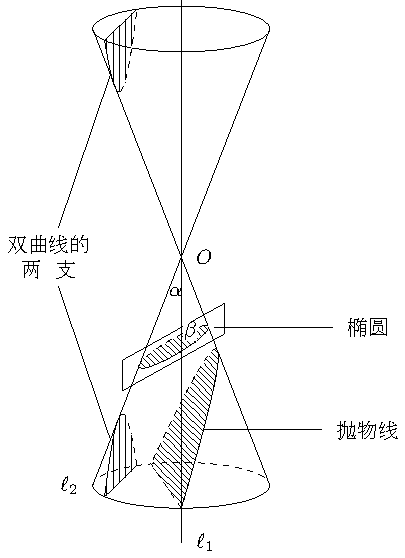
\includegraphics{2-conic-section-all.pdf}
    \caption{}
    \end{minipage}
\end{figure}

设$P$是椭圆截痕上任一点,则过$P$点与轴线平行的直线
全在柱面上,设它交圆$C_1$和圆$C_2$于$Q_1$和$Q_2$两点,则
\begin{itemize}
    \item $PQ_1$和$PF_1$是$P$点到上球的两条切线,所以等长.
    \item   $PQ_2$和$PF_2$是$P$点到下球的两条切线,所以等长.
\end{itemize}

所以,$PF_1+PF_2=PQ_1+PQ_2=Q_1Q_2$

我们让$P$点在椭圆上
变动,则$Q_1Q_2$的变化只
是绕轴旋转,而其长度保持不变的.这就是说,
$PF_1+PF_2=Q_1Q_2=$常数.

$F_1$、$F_2$椭圆焦点,这
就发现了椭圆的特性:椭
圆是平面上一个动点到两个定点$F_1$和$F_2$的距离之
和等于定长的轨迹,$F_1$和
$F_2$叫做椭圆的焦点.

\subsection{圆锥与圆锥曲线}

设$\ell_1$、$\ell_2$是相交于$O$点的两条直线,让$\ell_2$以$\ell_1$为旋转
所得的曲面就是一个圆锥面.再用不过$O$点的平面去截割圆
锥面,所得的曲线叫圆锥曲线,如图2.82所示.设$\ell_1$、$\ell_2$的夹角
为$\alpha$, 截平面和轴的交角为$\beta$, 则不难发现$\beta>\alpha$时,截痕为
椭圆;$\beta=\alpha$时,截痕为抛物线;$\beta<\alpha$时,截痕分为上、下
两支,是双曲线.这三类曲线统称圆锥曲线(或圆锥截线).
这样就对上述这三种曲线有了一种统一的产生办法和处理方
式.

\subsection{圆锥曲线的性质}
在一中前面我们用平面斜截圆柱面而得椭圆这一类型的曲
线,并且利用上、下切球和定点到球面的切线长相等来推导
它的性质:
$PF_1+PF_2=$定长.

在二中我们改用平面来截割圆锥面来构造三种曲线,
其中$\beta>\alpha$时,我们说所得曲线
还是椭圆,这一点还得加以证
明.现在我们把一中的证明略作
修改,证明如下:

我们依然可以作一个
上切球,它和圆锥面相切于圆
$C_1$, 和截割平面相切于$F_1$点,
也可以作一个下切球,它和圆锥
面相切于圆$C_2$, 和截割平面相切
于$F_2$点(唯一不同之点是:
在柱面的情形,上下切球大小相
同,这里的上、下切球一小,一
大.如图2.83).

设$P$为截痕上任意一点,连结直线$OP$, 交$C_1$、$C_2$于$Q_1$
和$Q_2$两点,则同样有
\[PQ_1=PF_1,\qquad PQ_2=PF_2\]
所以$PF_1+PF_2=Q_1Q_2$.

再者,当$P$点在截痕上变动时,$Q_1Q_2$的变化只在锥面上
旋转,而长度不变.这就证明了圆锥的这种截痕($\beta>\alpha$)
满足一中所证的椭圆的性质,因此它也是椭圆.

\begin{figure}[htp]\centering
    \begin{minipage}[t]{0.48\textwidth}
    \centering
    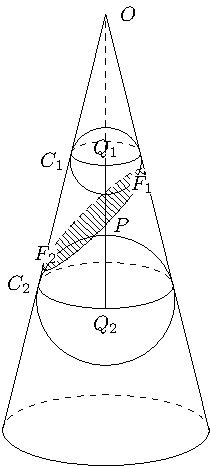
\includegraphics{2-conic-section-ellipse.pdf}
    \caption{}
    \end{minipage}
    \begin{minipage}[t]{0.48\textwidth}
    \centering
    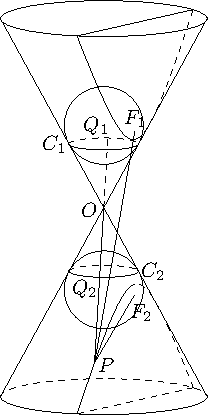
\includegraphics{2-conic-section-hyperbola.pdf}
    \caption{}
    \end{minipage}
    \end{figure}

\subsubsection{双曲线的性质}
设$\beta<\alpha$, 则截割平面交圆锥于上、下两支,如图2.84所
示,我们也可以作上、下两个切球(这次它们分居于圆锥的
上、下两部),它们和圆锥分别切于圆$C_1$和圆$C_2$, 和截平面
相切于$F_1$和$F_2$点.

设$P$为截痕上的任一点,连结直线$OP$, 分别交$C_1$、$C_2$
于$Q_1$和$Q_2$点,则同样地可以得出:
\[PF_1=PQ_1,\qquad PF_2=PQ_2\]
而$QQ_2$的长度是与$P$点位置无关的一个常数,
所以,$Q_1Q_2=PQ_1-PQ_2=PF_1-PF_2=$常数.

这就证明了双曲线的性质:双曲线上的任一点和双曲线
所在平面上两个定点的距离之差等于一个常数.
即
\[PF_1-PF_2=\text{常数}\qquad \text{或}\qquad PF_2-PF_1=\text{常数}\]


\subsubsection{抛物线的性质}
设$\beta=\alpha$, 则截割平面和圆锥交于开口的一支,这时我
们只能作一个球,它和圆锥相交于$C$, 和截平面相切于$F$点.

再者,圆$C$所在的平面和截平面相交于一条直线叫作
准线,如图2.85所示\footnote{原课本插图中$P'Q'$为圆锥左侧母线,这不准确. 为使$P'Q'$与$PR$平行, $P'Q'$在底面上的投影须与抛物线截线正交, 故$P'Q'$不能为图示的左母线. 这已在新插图中订正.}.
\begin{figure}[ht]
    \centering
    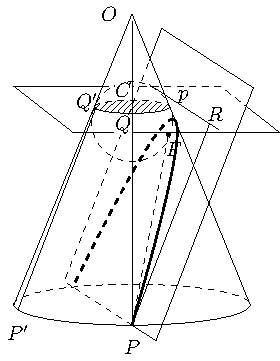
\includegraphics{2-conic-section-parabola.pdf}
    \caption{}
\end{figure}

设$P$是截痕上任一点,连结$PO$交圆$C$于$Q$点,再由$P$点
向准线$p$作垂线$PR$. 由假设,我们可以将$PQ$旋转到和$PR$
平行的位置$P'Q'$, 这样,就不难看出:
\begin{itemize}
    \item $PF=PQ$(切线长相等)
    \item $PQ=P'Q'$(移形公理)
    \item $PR=P'Q'$(平行平面间的平行线段相等)
\end{itemize}

所以$PF=PR=P$点到准线的距离.

总结上面的讨论得到抛物线的性质:
抛物线上任意一点和抛物线所在平面上的一定点和一定
直线的距离相等.即:$PF=PR$.

定点叫作抛物线的焦点,定直线叫做它的准线.

